


%% need no \usepackage{Sweave.sty}



%




%% use JSS class -- use 'nojss' to turn off header
\documentclass[shortnames,nojss,article]{jss}\usepackage[]{graphicx}\usepackage[]{color}
%% maxwidth is the original width if it is less than linewidth
%% otherwise use linewidth (to make sure the graphics do not exceed the margin)
\makeatletter
\def\maxwidth{ %
  \ifdim\Gin@nat@width>\linewidth
    \linewidth
  \else
    \Gin@nat@width
  \fi
}
\makeatother

\definecolor{fgcolor}{rgb}{0.345, 0.345, 0.345}
\newcommand{\hlnum}[1]{\textcolor[rgb]{0.686,0.059,0.569}{#1}}%
\newcommand{\hlstr}[1]{\textcolor[rgb]{0.192,0.494,0.8}{#1}}%
\newcommand{\hlcom}[1]{\textcolor[rgb]{0.678,0.584,0.686}{\textit{#1}}}%
\newcommand{\hlopt}[1]{\textcolor[rgb]{0,0,0}{#1}}%
\newcommand{\hlstd}[1]{\textcolor[rgb]{0.345,0.345,0.345}{#1}}%
\newcommand{\hlkwa}[1]{\textcolor[rgb]{0.161,0.373,0.58}{\textbf{#1}}}%
\newcommand{\hlkwb}[1]{\textcolor[rgb]{0.69,0.353,0.396}{#1}}%
\newcommand{\hlkwc}[1]{\textcolor[rgb]{0.333,0.667,0.333}{#1}}%
\newcommand{\hlkwd}[1]{\textcolor[rgb]{0.737,0.353,0.396}{\textbf{#1}}}%

\usepackage{framed}
\makeatletter
\newenvironment{kframe}{%
 \def\at@end@of@kframe{}%
 \ifinner\ifhmode%
  \def\at@end@of@kframe{\end{minipage}}%
  \begin{minipage}{\columnwidth}%
 \fi\fi%
 \def\FrameCommand##1{\hskip\@totalleftmargin \hskip-\fboxsep
 \colorbox{shadecolor}{##1}\hskip-\fboxsep
     % There is no \\@totalrightmargin, so:
     \hskip-\linewidth \hskip-\@totalleftmargin \hskip\columnwidth}%
 \MakeFramed {\advance\hsize-\width
   \@totalleftmargin\z@ \linewidth\hsize
   \@setminipage}}%
 {\par\unskip\endMakeFramed%
 \at@end@of@kframe}
\makeatother

\definecolor{shadecolor}{rgb}{.97, .97, .97}
\definecolor{messagecolor}{rgb}{0, 0, 0}
\definecolor{warningcolor}{rgb}{1, 0, 1}
\definecolor{errorcolor}{rgb}{1, 0, 0}
\newenvironment{knitrout}{}{} % an empty environment to be redefined in TeX

\usepackage{alltt}
\usepackage{booktabs,flafter,thumbpdf}
%\VignetteIndexEntry{An Introduction to dendextend}
%\VignetteKeywords{Dendrogram, hclust, heirarchical clustering, visualization, tanglegram, R}
%\VignettePackage{dendextend}
%\VignetteEngine{knitr::knitr}



\Plaintitle{Visualizing and Comparing Trees of Heirarchical Clustering: Using the dendextend R Package}
\title{Visualizing and Comparing\\ Trees of Heirarchical Clustering:\\ Using the dendextend \proglang{R} Package}


% \Plaintitle{Manipulate, Visualize and Compare Dendrograms: The dendextend R Package}
% \title{Manipulate, Visualize and Compare Dendrograms:\\ The \pkg{dendextend} \proglang{R} Package}


\author{Tal Galili\\Tel-Aviv University \And Yoav Benjamini\\Tel-Aviv University}
\Plainauthor{Tal Galili, Yoav Benjamini}



\Abstract{

A dendrogram is a tree diagram which is often used to visualize an hierarchical clustering of items. Dendrograms are used in many dispelines, ranging from Phylogenetic Trees in computational biology to Lexomic Trees in text analysis.

The \pkg{dendextend} package extends the dendrogram objects in the \proglang{R} programming language, allowing for easy manipulation of a dendrogram's shape, color and content. Furthermore, it enable the tools for comparing the similarity of two dendrograms to one another both graphically (using tanglegrems) and statistically (from cophenetic correlations to Bk plots).

The paper gives a detailed exposition of both the internal structure of the package and the provided user interfaces.
}

\Keywords{Dendrogram, hclust, hierarchical clustering, visualization, tanglegram,  \proglang{R}}
\Plainkeywords{Dendrogram, hclust, hierarchical clustering, visualization, tanglegram, R}


% \begin{center} \today \end{center}.

% \Volume{40}
% \Issue{8}
% \Month{April}
% \Year{2011}
% \Submitdate{2010-11-15}
% \Acceptdate{2011-03-21}

\Address{
  Tal Galili \\
   Department of Statistics and Operations Research \\
   Tel Aviv University, Israel \\
   E-mail: \email{tal.galili@math.tau.ac.il}\\
   URLs: \url{http://www.r-statistics.com/}, 
         \url{http://www.r-bloggers.com/}\\

  Yoav Benjamini\\
   The Nathan and Lily Silver\\
   Professor of Applied Statistics\\
   Department of Statistics and Operations Research \\
   Tel Aviv University, Israel \\
   E-mail: \email{ybenja@tau.ac.il}\\
   URL: \url{http://www.tau.ac.il/~ybenja/}
}
\IfFileExists{upquote.sty}{\usepackage{upquote}}{}



\begin{document}
\vspace*{-0.25cm}

%% Doesn't seem to work:
%% \tableofcontents


\section{Introduction}

\subsection{The \code{dendrogram} object}

The \code{dendrogram} class provides general functions for handling tree-like structures in \proglang{R} \citep{R:Main}. It is intended as a replacement for similar functions in hierarchical clustering and classification/regression trees, such that all of these can use the same engine for plotting or cutting trees.

A dendrogram object represents a tree as a nested \code{list} object, with various attributes.

Dendrogram has several useful methods bundled with R:

\begin{knitrout}
\definecolor{shadecolor}{rgb}{0.969, 0.969, 0.969}\color{fgcolor}\begin{kframe}
\begin{alltt}
\hlkwd{methods}\hlstd{(}\hlkwc{class} \hlstd{=} \hlstr{"dendrogram"}\hlstd{)}
\end{alltt}
\begin{verbatim}
##  [1] [[.dendrogram*           as.hclust.dendrogram*   
##  [3] as.phylo.dendrogram      cophenetic.dendrogram*  
##  [5] cut.dendrogram*          cutree.dendrogram       
##  [7] entanglement.dendrogram* head.dendrogram*        
##  [9] labels.dendrogram*       labels<-.dendrogram     
## [11] merge.dendrogram*        nleaves.dendrogram*     
## [13] nnodes.dendrogram*       plot.dendrogram*        
## [15] print.dendrogram*        reorder.dendrogram*     
## [17] rev.dendrogram*          rotate.dendrogram*      
## [19] sort.dendrogram*         str.dendrogram*         
## [21] tanglegram.dendrogram*   trim.dendrogram*        
## [23] unbranch.dendrogram*    
## 
##    Non-visible functions are asterisked
\end{verbatim}
\end{kframe}
\end{knitrout}


For example, let's create a dendrogram object based on an hierarchical clustering of 4 states in the U.S.:

\begin{knitrout}
\definecolor{shadecolor}{rgb}{0.969, 0.969, 0.969}\color{fgcolor}\begin{kframe}
\begin{alltt}
\hlcom{# our data:}
\hlkwd{data}\hlstd{(USArrests)}
\hlstd{US_data} \hlkwb{<-} \hlstd{USArrests[}\hlkwd{c}\hlstd{(}\hlnum{2}\hlstd{,} \hlnum{5}\hlstd{,} \hlnum{32}\hlstd{,} \hlnum{35}\hlstd{), ]}
\hlkwd{print}\hlstd{(US_data)}
\end{alltt}
\begin{verbatim}
##            Murder Assault UrbanPop Rape
## Alaska       10.0     263       48 44.5
## California    9.0     276       91 40.6
## New York     11.1     254       86 26.1
## Ohio          7.3     120       75 21.4
\end{verbatim}
\begin{alltt}
\hlstd{hc} \hlkwb{<-} \hlkwd{hclust}\hlstd{(}\hlkwd{dist}\hlstd{(US_data),} \hlstr{"ave"}\hlstd{)}  \hlcom{# create an heirarchical clustering object}
\hlstd{dend} \hlkwb{<-} \hlkwd{as.dendrogram}\hlstd{(hc)}
\end{alltt}
\end{kframe}
\end{knitrout}



Below are examples for some dendrogram methods:

\begin{knitrout}
\definecolor{shadecolor}{rgb}{0.969, 0.969, 0.969}\color{fgcolor}\begin{kframe}
\begin{alltt}
\hlkwd{print}\hlstd{(dend)}
\end{alltt}
\begin{verbatim}
## 'dendrogram' with 2 branches and 4 members total, at height 146.7
\end{verbatim}
\begin{alltt}
\hlkwd{labels}\hlstd{(dend)}
\end{alltt}
\begin{verbatim}
## [1] "Ohio"       "Alaska"     "California" "New York"
\end{verbatim}
\begin{alltt}
\hlkwd{str}\hlstd{(dend)}
\end{alltt}
\begin{verbatim}
## --[dendrogram w/ 2 branches and 4 members at h = 147]
##   |--leaf "Ohio" 
##   `--[dendrogram w/ 2 branches and 3 members at h = 44.1]
##      |--leaf "Alaska" 
##      `--[dendrogram w/ 2 branches and 2 members at h = 26.9]
##         |--leaf "California" 
##         `--leaf "New York"
\end{verbatim}
\begin{alltt}
\hlkwd{str}\hlstd{(dend[[}\hlnum{2}\hlstd{]])}  \hlcom{# looking at one branch of the dendrogram}
\end{alltt}
\begin{verbatim}
## --[dendrogram w/ 2 branches and 3 members at h = 44.1]
##   |--leaf "Alaska" 
##   `--[dendrogram w/ 2 branches and 2 members at h = 26.9]
##      |--leaf "California" 
##      `--leaf "New York"
\end{verbatim}
\begin{alltt}
\hlkwd{plot}\hlstd{(dend)}
\end{alltt}
\end{kframe}

{\centering 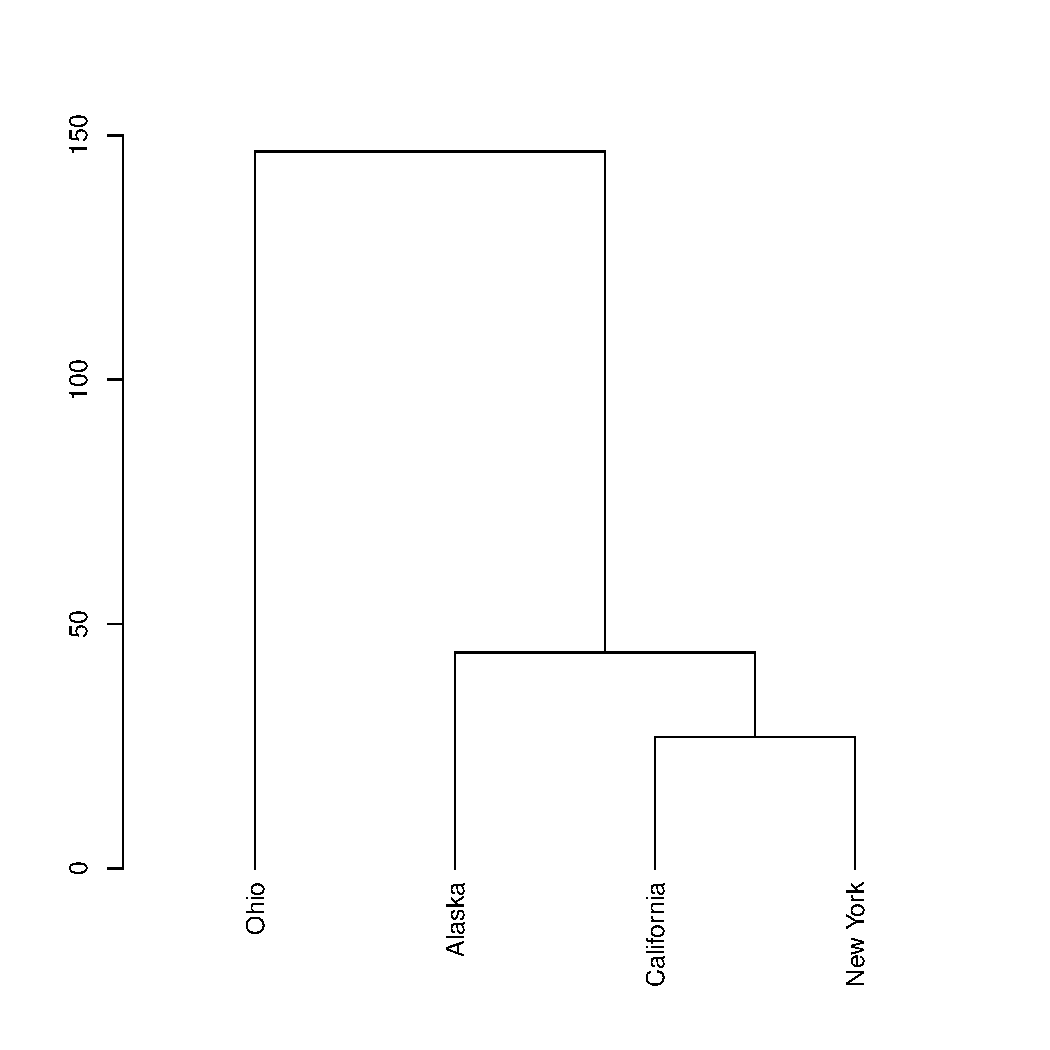
\includegraphics[width=4in,height=4in]{figure/unnamed-chunk-4} 

}



\end{knitrout}


You might notice how the order of the items (leaves/terminal nodes) of the dendrogram is different than their order in the table. In order to re-order the rows in the data-table to have the same order as the items in the dendrogram, we can use the \code{order.dendrogram} function:

\begin{knitrout}
\definecolor{shadecolor}{rgb}{0.969, 0.969, 0.969}\color{fgcolor}\begin{kframe}
\begin{alltt}
\hlstd{(new_order} \hlkwb{<-} \hlkwd{order.dendrogram}\hlstd{(dend))}
\end{alltt}
\begin{verbatim}
## [1] 4 1 2 3
\end{verbatim}
\begin{alltt}
\hlcom{# the order of the original items to have them be at the same}
\hlcom{# order as they assume in the dendrogram}
\hlkwd{print}\hlstd{(US_data[new_order, ])}
\end{alltt}
\begin{verbatim}
##            Murder Assault UrbanPop Rape
## Ohio          7.3     120       75 21.4
## Alaska       10.0     263       48 44.5
## California    9.0     276       91 40.6
## New York     11.1     254       86 26.1
\end{verbatim}
\end{kframe}
\end{knitrout}



In order to see what our dendrogram (\code{list}) object includes, we need to use the \code{unclass} function, which will strip away the class attribute and will allow us to print the list as is, without going through the \code{print.dendrogram} method. We can see how each node in the dendrogram/list object has the following (self explaining) attributes:

\begin{knitrout}
\definecolor{shadecolor}{rgb}{0.969, 0.969, 0.969}\color{fgcolor}\begin{kframe}
\begin{alltt}
\hlkwd{str}\hlstd{(}\hlkwd{unclass}\hlstd{(dend))}
\end{alltt}
\begin{verbatim}
## List of 2
##  $ : atomic [1:1] 4
##   ..- attr(*, "members")= int 1
##   ..- attr(*, "height")= num 0
##   ..- attr(*, "label")= chr "Ohio"
##   ..- attr(*, "leaf")= logi TRUE
##  $ :List of 2
##   ..$ : atomic [1:1] 1
##   .. ..- attr(*, "members")= int 1
##   .. ..- attr(*, "height")= num 0
##   .. ..- attr(*, "label")= chr "Alaska"
##   .. ..- attr(*, "leaf")= logi TRUE
##   ..$ :List of 2
##   .. ..$ : atomic [1:1] 2
##   .. .. ..- attr(*, "label")= chr "California"
##   .. .. ..- attr(*, "members")= int 1
##   .. .. ..- attr(*, "height")= num 0
##   .. .. ..- attr(*, "leaf")= logi TRUE
##   .. ..$ : atomic [1:1] 3
##   .. .. ..- attr(*, "label")= chr "New York"
##   .. .. ..- attr(*, "members")= int 1
##   .. .. ..- attr(*, "height")= num 0
##   .. .. ..- attr(*, "leaf")= logi TRUE
##   .. ..- attr(*, "members")= int 2
##   .. ..- attr(*, "midpoint")= num 0.5
##   .. ..- attr(*, "height")= num 26.9
##   ..- attr(*, "members")= int 3
##   ..- attr(*, "midpoint")= num 0.75
##   ..- attr(*, "height")= num 44.1
##  - attr(*, "members")= int 4
##  - attr(*, "midpoint")= num 0.875
##  - attr(*, "height")= num 147
\end{verbatim}
\end{kframe}
\end{knitrout}



Notice how terminal nodes uses the "leaf" attribute (set to TRUE).
\begin{knitrout}
\definecolor{shadecolor}{rgb}{0.969, 0.969, 0.969}\color{fgcolor}\begin{kframe}
\begin{alltt}
\hlkwd{names}\hlstd{(}\hlkwd{attributes}\hlstd{(dend)[}\hlopt{-}\hlnum{4}\hlstd{])}
\end{alltt}
\begin{verbatim}
## [1] "members"  "midpoint" "height"
\end{verbatim}
\end{kframe}
\end{knitrout}




A very important function is \code{dendrapply}. It applies some function recursively to each node of a dendrogram. It is often used for adjusting attributes of the object, or extracting something from it. 

One current "feature" with this function is that just sending a dendrogram through it will return it with each of its nodes becoming of class "dendrogram". Notice the use of the \code{unclass_dend} function. Example:

\begin{knitrout}
\definecolor{shadecolor}{rgb}{0.969, 0.969, 0.969}\color{fgcolor}\begin{kframe}
\begin{alltt}
\hlcom{# dendrapply(dend, unclass) # in case the}
\hlstd{itself} \hlkwb{<-} \hlkwa{function}\hlstd{(}\hlkwc{x}\hlstd{) x}
\hlstd{dend_from_dendrapply} \hlkwb{<-} \hlkwd{dendrapply}\hlstd{(dend, itself}\hlstd{)}

\hlcom{# here we must first use unclass since '[[]]' inherits its}
\hlcom{# class to the output:}
\hlkwd{class}\hlstd{(}\hlkwd{unclass}\hlstd{(dend)[[}\hlnum{2}\hlstd{]])}
\end{alltt}
\begin{verbatim}
## [1] "list"
\end{verbatim}
\begin{alltt}
\hlkwd{class}\hlstd{(}\hlkwd{unclass}\hlstd{(dend_from_dendrapply)[[}\hlnum{2}\hlstd{]])}
\end{alltt}
\begin{verbatim}
## [1] "dendrogram"
\end{verbatim}
\begin{alltt}
\hlkwd{class}\hlstd{(}\hlkwd{unclass_dend}\hlstd{(dend_from_dendrapply)[[}\hlnum{2}\hlstd{]])}  \hlcom{# the new uncless_dend solves it.}
\end{alltt}
\begin{verbatim}
## [1] "list"
\end{verbatim}
\end{kframe}
\end{knitrout}




\subsection{Motivation for creating \code{dendextend}}



The \code{dendrogram} object has several \textbf{advantages}:

\begin{enumerate}

   \item \code{dendrogram} objects are list R objects. This makes their structure very familiar and easy to understand by R users. They are also, relatively, simple to manipulate and extend.
   \item \code{dendrogram} objects has various methods and functions for using them within R base. 
   \item Other tree objects, such as \code{hclust}, and objects from the \pkg{ape} package \citep{CRAN:ape},  include an \code{as.dendrogram} method for converting their objects into a dendrogram. And also \code{as.phylo.dendrogram}, \code{as.hclust.dendrogram}.
   \item \code{dendrogram} objects are used in various packages as an intermediate step for other purposes (often plotting), such as:
   
   \begin{enumerate}
   \item The \pkg{latticeExtra} package \citep{CRAN:latticeExtra}, see the \code{dendrogramGrob} function.
   \item The \pkg{labeltodendro} package \citep{CRAN:labeltodendro}, see the \code{colorplot} function.
   \item The \pkg{bclust} package \citep{CRAN:bclust}, see the \code{bclust} function.
   \item The \pkg{ggdendro} package \citep{CRAN:ggdendro}, see the \code{dendro_data} function.
   \item The \pkg{Heatplus} package \citep{CRAN:Heatplus}, see the \code{annHeatmap2} function.
   \item The \pkg{sparcl} package \citep{CRAN:Heatplus}, see the \code{ColorDendrogram} function.
   \end{enumerate}
   
\end{enumerate}
   
   %\pkg{DendSer} (see the \code{} function), 


However, even with all of its advantages, the \code{dendrogram} class in R still lacks various basic features.

The \code{dendextend} package aims at filling some gaps in base R, by extending the available functions for dendrogram manipulation, statistical analysis, and visualization.

This vignettes Provides a step-by-step description of the functionality provided by the \code{dendextend} package.


\subsection{Installing \code{dendextend}}

To install the stable version from CRAN use:

\begin{knitrout}
\definecolor{shadecolor}{rgb}{0.969, 0.969, 0.969}\color{fgcolor}\begin{kframe}
\begin{alltt}
\hlkwd{install.packages}\hlstd{(}\hlstr{"dendextend"}\hlstd{)}  \hlcom{# not yet available from CRAN}
\end{alltt}
\end{kframe}
\end{knitrout}



To install the \href{https://github.com/talgalili/dendextend}{GitHub version} use:

\begin{knitrout}
\definecolor{shadecolor}{rgb}{0.969, 0.969, 0.969}\color{fgcolor}\begin{kframe}
\begin{alltt}
\hlkwa{if} \hlstd{(}\hlopt{!}\hlkwd{require}\hlstd{(}\hlstr{"devtools"}\hlstd{))} \hlkwd{install.packages}\hlstd{(}\hlstr{"devtools"}\hlstd{)}
\hlkwd{require}\hlstd{(}\hlstr{"devtools"}\hlstd{)}
\hlkwd{install_github}\hlstd{(}\hlstr{"dendextend"}\hlstd{,} \hlstr{"talgalili"}\hlstd{)}
\end{alltt}
\end{kframe}
\end{knitrout}



\section{Tree attributes (extraction, assignment, length)}


\subsection{labels in base R}

In base R, the \code{labels} function is intended to find/extract a suitable set of labels from an object for use in printing or plotting, for example. By default, it uses the \code{names} and \code{dimnames} functions.

What base R \code{labels} function is missing is assignment. In the next few examples we will go through different examples of what the \code{dendextend} package offers for various objects.

\textbf{Credits:} These assignment functions were originally written by Gavin Simpson (in a post on \href{http://stackoverflow.com/questions/4614223/how-to-have-the-following-work-labelsx-some-value-r-question}{(stackoverflow)}), and adopted/adjusted to this package by Tal Galili. Some modification were inspired by Gregory Jefferis's code from the \pkg{dendroextras} package.


\subsection{labels for vectors and matrices}

In base R, for vectors, labels gives the \code{names} of the object. And if these are missing, then \code{labels} will give the vector itself as a character vector:

\begin{knitrout}
\definecolor{shadecolor}{rgb}{0.969, 0.969, 0.969}\color{fgcolor}\begin{kframe}
\begin{alltt}
\hlstd{x} \hlkwb{<-} \hlnum{1}\hlopt{:}\hlnum{3}
\hlkwd{names}\hlstd{(x)}  \hlcom{# this vector has no names}
\end{alltt}
\begin{verbatim}
## NULL
\end{verbatim}
\begin{alltt}
\hlkwd{labels}\hlstd{(x)}  \hlcom{# this vector has no labels}
\end{alltt}
\begin{verbatim}
## [1] "1" "2" "3"
\end{verbatim}
\end{kframe}
\end{knitrout}


Assignment to names is available in base R and works as follows:

\begin{knitrout}
\definecolor{shadecolor}{rgb}{0.969, 0.969, 0.969}\color{fgcolor}\begin{kframe}
\begin{alltt}
\hlstd{x} \hlkwb{<-} \hlnum{1}\hlopt{:}\hlnum{3}
\hlkwd{names}\hlstd{(x)} \hlkwb{<-} \hlstd{letters[}\hlnum{1}\hlopt{:}\hlnum{3}\hlstd{]}  \hlcom{# assignment for names is in base R}
\hlcom{# both names and labels will give the same result:}
\hlkwd{names}\hlstd{(x)}
\end{alltt}
\begin{verbatim}
## [1] "a" "b" "c"
\end{verbatim}
\begin{alltt}
\hlkwd{labels}\hlstd{(x)}
\end{alltt}
\begin{verbatim}
## [1] "a" "b" "c"
\end{verbatim}
\end{kframe}
\end{knitrout}



The new labels assignment function will allow a user to change the labels of the vector just as if it was "names":

\begin{knitrout}
\definecolor{shadecolor}{rgb}{0.969, 0.969, 0.969}\color{fgcolor}\begin{kframe}
\begin{alltt}
\hlstd{x} \hlkwb{<-} \hlnum{1}\hlopt{:}\hlnum{3}
\hlkwd{labels}\hlstd{(x)} \hlkwb{<-} \hlstd{letters[}\hlnum{1}\hlopt{:}\hlnum{3}\hlstd{]}
\hlkwd{names}\hlstd{(x)}
\end{alltt}
\begin{verbatim}
## [1] "a" "b" "c"
\end{verbatim}
\begin{alltt}
\hlkwd{labels}\hlstd{(x)}
\end{alltt}
\begin{verbatim}
## [1] "a" "b" "c"
\end{verbatim}
\end{kframe}
\end{knitrout}


Labels assignment are also available for matrices.


\subsection{labels for dendrogram objects}

We can get a dendrogram's labels using the \code{labels} function from base R. However, in order to assign new values to it, we'll need the assignment function from \pkg{dendextend}:

\begin{knitrout}
\definecolor{shadecolor}{rgb}{0.969, 0.969, 0.969}\color{fgcolor}\begin{kframe}
\begin{alltt}
\hlkwd{labels}\hlstd{(dend)}  \hlcom{# from base R}
\end{alltt}
\begin{verbatim}
## [1] "Ohio"       "Alaska"     "California" "New York"
\end{verbatim}
\begin{alltt}
\hlkwd{set.seed}\hlstd{(}\hlnum{2354235}\hlstd{)}
\hlkwd{labels}\hlstd{(dend)} \hlkwb{<-} \hlkwd{sample}\hlstd{(}\hlkwd{labels}\hlstd{(dend))}  \hlcom{# labels assingment - thanks to dendextend}
\hlkwd{labels}\hlstd{(dend)}
\end{alltt}
\begin{verbatim}
## [1] "New York"   "Ohio"       "Alaska"     "California"
\end{verbatim}
\end{kframe}
\end{knitrout}



\subsection{labels for hclust objects}

\pkg{dendextend} offers a \code{labels} method for \code{hclust} objects. It take special care to have the order of the labels be the same as is with dendrogram object, which is the order of the labels in the plotted tree. This can be turned off when using the \code{order} parameter:

\begin{knitrout}
\definecolor{shadecolor}{rgb}{0.969, 0.969, 0.969}\color{fgcolor}\begin{kframe}
\begin{alltt}
\hlcom{# All are from dendextend}
\hlkwd{labels}\hlstd{(hc)}
\end{alltt}
\begin{verbatim}
## [1] "Ohio"       "Alaska"     "California" "New York"
\end{verbatim}
\begin{alltt}
\hlkwd{labels}\hlstd{(hc,} \hlkwc{order} \hlstd{=} \hlnum{FALSE}\hlstd{)}  \hlcom{# this is the order of the rows of the original data.}
\end{alltt}
\begin{verbatim}
## [1] "Alaska"     "California" "New York"   "Ohio"
\end{verbatim}
\begin{alltt}
\hlkwd{set.seed}\hlstd{(}\hlnum{229835}\hlstd{)}
\hlkwd{labels}\hlstd{(hc)} \hlkwb{<-} \hlkwd{sample}\hlstd{(}\hlkwd{labels}\hlstd{(hc))}  \hlcom{# labels assingment - thanks to dendextend}
\hlkwd{labels}\hlstd{(hc)}
\end{alltt}
\begin{verbatim}
## [1] "California" "New York"   "Alaska"     "Ohio"
\end{verbatim}
\end{kframe}
\end{knitrout}



\subsection{labels assignment and recycling}

When the assigned vector has a different length, the \pkg{dendextend} assignment functions will recycle the value but also give a warning:

\begin{knitrout}
\definecolor{shadecolor}{rgb}{0.969, 0.969, 0.969}\color{fgcolor}\begin{kframe}
\begin{alltt}
\hlstd{x} \hlkwb{<-} \hlnum{1}\hlopt{:}\hlnum{3}
\hlstd{hc} \hlkwb{<-} \hlkwd{hclust}\hlstd{(}\hlkwd{dist}\hlstd{(US_data),} \hlstr{"ave"}\hlstd{)}
\hlstd{dend} \hlkwb{<-} \hlkwd{as.dendrogram}\hlstd{(hc)}
\hlstd{y} \hlkwb{<-} \hlkwd{matrix}\hlstd{(}\hlnum{1}\hlopt{:}\hlnum{9}\hlstd{,} \hlnum{3}\hlstd{,} \hlnum{3}\hlstd{)}

\hlkwd{labels}\hlstd{(x)} \hlkwb{<-} \hlstr{"bob"}
\end{alltt}


{\ttfamily\noindent\color{warningcolor}{\#\# Warning: The lengths of the new labels is shorter than the length of the object - labels are recycled.}}\begin{alltt}
\hlkwd{labels}\hlstd{(x)}
\end{alltt}
\begin{verbatim}
## [1] "bob" "bob" "bob"
\end{verbatim}
\begin{alltt}
\hlkwd{labels}\hlstd{(hc)} \hlkwb{<-} \hlstr{"bob"}
\end{alltt}


{\ttfamily\noindent\color{warningcolor}{\#\# Warning: The lengths of the new labels is shorter than the number of leaves in the hclust - labels are recycled.}}\begin{alltt}
\hlkwd{labels}\hlstd{(hc)}
\end{alltt}
\begin{verbatim}
## [1] "bob" "bob" "bob" "bob"
\end{verbatim}
\begin{alltt}
\hlkwd{labels}\hlstd{(dend)} \hlkwb{<-} \hlstr{"bob"}
\end{alltt}


{\ttfamily\noindent\color{warningcolor}{\#\# Warning: The lengths of the new labels is shorter than the number of leaves in the dendrogram - labels are recycled.}}\begin{alltt}
\hlkwd{labels}\hlstd{(dend)}
\end{alltt}
\begin{verbatim}
## [1] "bob" "bob" "bob" "bob"
\end{verbatim}
\begin{alltt}
\hlkwd{labels}\hlstd{(y)} \hlkwb{<-} \hlstr{"bob"}
\end{alltt}


{\ttfamily\noindent\color{warningcolor}{\#\# Warning: The lengths of the new labels is shorter than the length of the object's colnames - labels are recycled.}}\begin{alltt}
\hlkwd{labels}\hlstd{(y)}
\end{alltt}
\begin{verbatim}
## [1] "bob" "bob" "bob"
\end{verbatim}
\end{kframe}
\end{knitrout}



\subsection{Tree size - number of leaves}

Getting the size of a tree (e.g: number of leaves/terminal-nodes) is good for validation of functions, and also when we wish to initiate a variable to later fill with data from the leaves. 

The \code{labels} function for dendrogram is expensive, since it uses recursion to get all of the tree's elements. If we are only interested in getting the tree size, it is better to use the \code{nleaves} function. It has an S3 method for hclust, dendrogram and phylo (from the \pkg{ape}):

\begin{knitrout}
\definecolor{shadecolor}{rgb}{0.969, 0.969, 0.969}\color{fgcolor}\begin{kframe}
\begin{alltt}
\hlkwd{nleaves}\hlstd{(hc)}
\end{alltt}
\begin{verbatim}
## [1] 4
\end{verbatim}
\begin{alltt}
\hlkwd{nleaves}\hlstd{(dend)}
\end{alltt}
\begin{verbatim}
## [1] 4
\end{verbatim}
\end{kframe}
\end{knitrout}


For dendrograms the speed improvement is about 10 times using \code{labels}, whereas for hclust, there is not any gain made by using \code{nleaves}. Here is a quick benchmark:

\begin{knitrout}
\definecolor{shadecolor}{rgb}{0.969, 0.969, 0.969}\color{fgcolor}\begin{kframe}
\begin{alltt}
\hlkwd{library}\hlstd{(microbenchmark)}
\hlkwd{microbenchmark}\hlstd{(}\hlkwd{nleaves}\hlstd{(dend),} \hlkwd{length}\hlstd{(}\hlkwd{labels}\hlstd{(dend)))}
\end{alltt}
\begin{verbatim}
## Unit: microseconds
##                  expr    min     lq median    uq   max
##         nleaves(dend)  24.64  25.76  26.88  30.8 212.8
##  length(labels(dend)) 390.83 396.99 400.35 406.5 951.3
##  neval
##    100
##    100
\end{verbatim}
\begin{alltt}
\hlkwd{microbenchmark}\hlstd{(}\hlkwd{nleaves}\hlstd{(hc),} \hlkwd{length}\hlstd{(}\hlkwd{labels}\hlstd{(hc)))}
\end{alltt}
\begin{verbatim}
## Unit: microseconds
##                expr   min    lq median    uq    max neval
##         nleaves(hc) 19.60 20.16  20.72 21.28  31.92   100
##  length(labels(hc)) 31.36 31.92  32.20 32.48 151.18   100
\end{verbatim}
\end{kframe}
\end{knitrout}


There are border-line cases where the node above some leaves is of height 0. In such a case, we would consider that node as a "terminal node", and in order to count the number of such terminal nodes we would use \code{count_terminal_nodes} function. For example:

\begin{knitrout}
\definecolor{shadecolor}{rgb}{0.969, 0.969, 0.969}\color{fgcolor}\begin{kframe}
\begin{alltt}
\hlstd{hc} \hlkwb{<-} \hlkwd{hclust}\hlstd{(}\hlkwd{dist}\hlstd{(USArrests[}\hlnum{1}\hlopt{:}\hlnum{3}\hlstd{, ]),} \hlstr{"ave"}\hlstd{)}
\hlstd{dend} \hlkwb{<-} \hlkwd{as.dendrogram}\hlstd{(hc}\hlstd{)}

\hlkwd{par}\hlstd{(}\hlkwc{mfrow} \hlstd{=} \hlkwd{c}\hlstd{(}\hlnum{1}\hlstd{,} \hlnum{2}\hlstd{)}\hlstd{)}

\hlcom{### Trivial case}
\hlkwd{count_terminal_nodes}\hlstd{(dend)}  \hlcom{# 3 terminal nodes}
\end{alltt}
\begin{verbatim}
## [1] 3
\end{verbatim}
\begin{alltt}
\hlkwd{length}\hlstd{(}\hlkwd{labels}\hlstd{(dend))}  \hlcom{# 3 - the same number}
\end{alltt}
\begin{verbatim}
## [1] 3
\end{verbatim}
\begin{alltt}
\hlkwd{plot}\hlstd{(dend,} \hlkwc{main} \hlstd{=} \hlstr{"This is considered a tree \textbackslash{}n with THREE terminal nodes/leaves"}\hlstd{)}

\hlcom{### NON-Trivial case}
\hlkwd{str}\hlstd{(dend)}
\end{alltt}
\begin{verbatim}
## --[dendrogram w/ 2 branches and 3 members at h = 54.8]
##   |--leaf "Arizona" 
##   `--[dendrogram w/ 2 branches and 2 members at h = 37.2]
##      |--leaf "Alabama" 
##      `--leaf "Alaska"
\end{verbatim}
\begin{alltt}
\hlkwd{attr}\hlstd{(dend[[}\hlnum{2}\hlstd{]],} \hlstr{"height"}\hlstd{)} \hlkwb{<-} \hlnum{0}
\hlkwd{count_terminal_nodes}\hlstd{(dend)}  \hlcom{# 2 terminal nodes, why? see this plot:}
\end{alltt}
\begin{verbatim}
## [1] 2
\end{verbatim}
\begin{alltt}
\hlcom{# while we have 3 leaves, in practice we have only 2 terminal}
\hlcom{# nodes (this is a feature, not a bug.)}
\hlkwd{plot}\hlstd{(dend,} \hlkwc{main} \hlstd{=} \hlstr{"This is considered a tree \textbackslash{}n with TWO terminal nodes only"}\hlstd{)}
\end{alltt}
\end{kframe}

{\centering 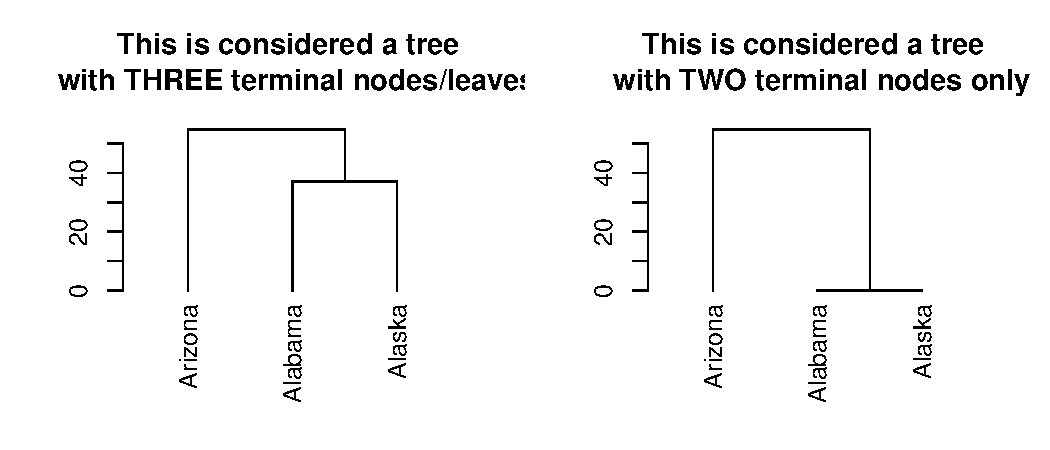
\includegraphics[width=\maxwidth]{figure/unnamed-chunk-19} 

}



\end{knitrout}



\subsection{Tree size - number of nodes}

Getting the size of a tree, in terms of the number of nodes can easily be done using:

\begin{knitrout}
\definecolor{shadecolor}{rgb}{0.969, 0.969, 0.969}\color{fgcolor}\begin{kframe}
\begin{alltt}
\hlstd{hc} \hlkwb{<-} \hlkwd{hclust}\hlstd{(}\hlkwd{dist}\hlstd{(USArrests[}\hlnum{1}\hlopt{:}\hlnum{3}\hlstd{, ]),} \hlstr{"ave"}\hlstd{)}
\hlstd{dend} \hlkwb{<-} \hlkwd{as.dendrogram}\hlstd{(hc}\hlstd{)}

\hlkwd{nnodes}\hlstd{(hc)}
\end{alltt}
\begin{verbatim}
## [1] 5
\end{verbatim}
\begin{alltt}
\hlkwd{nnodes}\hlstd{(dend)}
\end{alltt}
\begin{verbatim}
## [1] 5
\end{verbatim}
\end{kframe}
\end{knitrout}




\subsection{Generally getting tree attributes}

Getting tree attributes can more generally be achieved using \code{get_nodes_attr}, however, the dedicated function are often faster than the general solution. (also, in the future, we might introduce functions based on \pkg{Rcpp}, offering even faster times).

Here are some examples:

\begin{knitrout}
\definecolor{shadecolor}{rgb}{0.969, 0.969, 0.969}\color{fgcolor}\begin{kframe}
\begin{alltt}
\hlstd{hc} \hlkwb{<-} \hlkwd{hclust}\hlstd{(}\hlkwd{dist}\hlstd{(USArrests[}\hlnum{1}\hlopt{:}\hlnum{3}\hlstd{, ]),} \hlstr{"ave"}\hlstd{)}
\hlstd{dend} \hlkwb{<-} \hlkwd{as.dendrogram}\hlstd{(hc}\hlstd{)}

\hlcom{# get_leaves_attr(dend) # error :)}
\hlkwd{get_leaves_attr}\hlstd{(dend,} \hlstr{"label"}\hlstd{)}
\end{alltt}
\begin{verbatim}
## [1] "Arizona" "Alabama" "Alaska"
\end{verbatim}
\begin{alltt}
\hlkwd{labels}\hlstd{(dend,} \hlstr{"label"}\hlstd{)}
\end{alltt}
\begin{verbatim}
## [1] "Arizona" "Alabama" "Alaska"
\end{verbatim}
\begin{alltt}
\hlkwd{get_leaves_attr}\hlstd{(dend,} \hlstr{"height"}\hlstd{)}  \hlcom{# should be 0's}
\end{alltt}
\begin{verbatim}
## [1] 0 0 0
\end{verbatim}
\begin{alltt}
\hlkwd{get_nodes_attr}\hlstd{(dend,} \hlstr{"height"}\hlstd{)}
\end{alltt}
\begin{verbatim}
## [1] 54.80  0.00 37.18  0.00  0.00
\end{verbatim}
\begin{alltt}
\hlkwd{get_branches_heights}\hlstd{(dend,} \hlkwc{sort} \hlstd{=} \hlnum{FALSE}\hlstd{)}  \hlcom{# notice the sort=FALSE}
\end{alltt}
\begin{verbatim}
## [1] 54.80 37.18
\end{verbatim}
\begin{alltt}
\hlkwd{get_leaves_attr}\hlstd{(dend,} \hlstr{"leaf"}\hlstd{)}  \hlcom{# should be TRUE's}
\end{alltt}
\begin{verbatim}
## [1] TRUE TRUE TRUE
\end{verbatim}
\begin{alltt}
\hlkwd{get_nodes_attr}\hlstd{(dend,} \hlstr{"leaf"}\hlstd{)}  \hlcom{# conatins NA's}
\end{alltt}
\begin{verbatim}
## [1]   NA TRUE   NA TRUE TRUE
\end{verbatim}
\begin{alltt}
\hlkwd{get_nodes_attr}\hlstd{(dend,} \hlstr{"leaf"}\hlstd{,} \hlkwc{na.rm} \hlstd{=} \hlnum{TRUE}\hlstd{)}  \hlcom{# }
\end{alltt}
\begin{verbatim}
## [1] TRUE TRUE TRUE
\end{verbatim}
\begin{alltt}
\hlkwd{get_leaves_attr}\hlstd{(dend,} \hlstr{"members"}\hlstd{)}  \hlcom{# should be 1's}
\end{alltt}
\begin{verbatim}
## [1] 1 1 1
\end{verbatim}
\begin{alltt}
\hlkwd{get_nodes_attr}\hlstd{(dend,} \hlstr{"members"}\hlstd{,} \hlkwc{include_branches} \hlstd{=} \hlnum{FALSE}\hlstd{,} \hlkwc{na.rm} \hlstd{=} \hlnum{TRUE}\hlstd{)}  \hlcom{# }
\end{alltt}
\begin{verbatim}
## [1] 1 1 1
\end{verbatim}
\begin{alltt}
\hlkwd{get_nodes_attr}\hlstd{(dend,} \hlstr{"members"}\hlstd{)}  \hlcom{# }
\end{alltt}
\begin{verbatim}
## [1] 3 1 2 1 1
\end{verbatim}
\begin{alltt}
\hlkwd{get_nodes_attr}\hlstd{(dend,} \hlstr{"members"}\hlstd{,} \hlkwc{include_leaves} \hlstd{=} \hlnum{FALSE}\hlstd{,} \hlkwc{na.rm} \hlstd{=} \hlnum{TRUE}\hlstd{)}  \hlcom{# }
\end{alltt}
\begin{verbatim}
## [1] 3 2
\end{verbatim}
\begin{alltt}
\hlstd{hang_dend} \hlkwb{<-} \hlkwd{hang.dendrogram}\hlstd{(dend)}
\hlkwd{get_leaves_attr}\hlstd{(hang_dend,} \hlstr{"height"}\hlstd{)}  \hlcom{# no longer 0!}
\end{alltt}
\begin{verbatim}
## [1] 49.32 31.70 31.70
\end{verbatim}
\begin{alltt}
\hlkwd{get_nodes_attr}\hlstd{(hang_dend,} \hlstr{"height"}\hlstd{)}  \hlcom{# does not include any 0s!}
\end{alltt}
\begin{verbatim}
## [1] 54.80 49.32 37.18 31.70 31.70
\end{verbatim}
\begin{alltt}
\hlcom{# does not include leaves values:}
\hlkwd{get_nodes_attr}\hlstd{(hang_dend,} \hlstr{"height"}\hlstd{,} \hlkwc{include_leaves} \hlstd{=} \hlnum{FALSE}\hlstd{)}
\end{alltt}
\begin{verbatim}
## [1] 54.80    NA 37.18    NA    NA
\end{verbatim}
\begin{alltt}
\hlcom{# remove leaves values all together:}
\hlkwd{get_nodes_attr}\hlstd{(hang_dend,} \hlstr{"height"}\hlstd{,} \hlkwc{include_leaves} \hlstd{=} \hlnum{FALSE}\hlstd{,} \hlkwc{na.rm} \hlstd{=} \hlnum{TRUE}\hlstd{)}
\end{alltt}
\begin{verbatim}
## [1] 54.80 37.18
\end{verbatim}
\begin{alltt}
\hlkwd{get_branches_heights}\hlstd{(hang_dend)}  \hlcom{# notice the sort}
\end{alltt}
\begin{verbatim}
## [1] 37.18 54.80
\end{verbatim}
\begin{alltt}
\hlkwd{get_branches_heights}\hlstd{(hang_dend,} \hlkwc{sort} \hlstd{=} \hlnum{FALSE}\hlstd{)}  \hlcom{# notice the sort}
\end{alltt}
\begin{verbatim}
## [1] 54.80 37.18
\end{verbatim}
\begin{alltt}

\end{alltt}
\end{kframe}
\end{knitrout}



Quick comparison on fetching leaves attributes:

\begin{knitrout}
\definecolor{shadecolor}{rgb}{0.969, 0.969, 0.969}\color{fgcolor}\begin{kframe}
\begin{alltt}
\hlkwd{require}\hlstd{(microbenchmark)}
\hlcom{# get_leaves_attr is twice faster than get_nodes_attr}
\hlkwd{microbenchmark}\hlstd{(}\hlkwc{get_leaves_attr_4members} \hlstd{=} \hlkwd{get_leaves_attr}\hlstd{(dend,}
    \hlstr{"members"}\hlstd{),} \hlkwc{get_nodes_attr_4members} \hlstd{=} \hlkwd{get_nodes_attr}\hlstd{(dend,}
    \hlstr{"members"}\hlstd{,} \hlkwc{include_branches} \hlstd{=} \hlnum{FALSE}\hlstd{,} \hlkwc{na.rm} \hlstd{=} \hlnum{TRUE}\hlstd{))}
\end{alltt}
\begin{verbatim}
## Unit: microseconds
##                      expr   min    lq median    uq    max
##  get_leaves_attr_4members 290.6 295.1  300.7 324.2  444.6
##   get_nodes_attr_4members 708.9 717.3  732.4 786.1 2855.6
##  neval
##    100
##    100
\end{verbatim}
\begin{alltt}


\end{alltt}
\end{kframe}
\end{knitrout}







\section{Tree manipulation}

\subsection{unbranching and root height}

A tree's nodes has various heights. Sometimes we are interested in changing the height of the entire tree. It is useful when This can be accomplished using \code{raise.dendrogram}. For example (notice how the entire tree's height is changed):

\begin{knitrout}
\definecolor{shadecolor}{rgb}{0.969, 0.969, 0.969}\color{fgcolor}\begin{kframe}
\begin{alltt}
\hlstd{hc} \hlkwb{<-} \hlkwd{hclust}\hlstd{(}\hlkwd{dist}\hlstd{(USArrests[}\hlnum{1}\hlopt{:}\hlnum{3}\hlstd{, ]),} \hlstr{"ave"}\hlstd{)}
\hlstd{dend} \hlkwb{<-} \hlkwd{as.dendrogram}\hlstd{(hc}\hlstd{)}

\hlstd{taller_dend} \hlkwb{<-} \hlkwd{raise.dendrogram}\hlstd{(dend,} \hlnum{10}\hlstd{)}
\hlstd{shorter_dend} \hlkwb{<-} \hlkwd{raise.dendrogram}\hlstd{(dend,} \hlopt{-}\hlnum{10}\hlstd{)}

\hlkwd{attr}\hlstd{(dend,} \hlstr{"height"}\hlstd{)}  \hlcom{# 54.80041}
\end{alltt}
\begin{verbatim}
## [1] 54.8
\end{verbatim}
\begin{alltt}
\hlkwd{attr}\hlstd{(taller_dend,} \hlstr{"height"}\hlstd{)}  \hlcom{# 64.80041}
\end{alltt}
\begin{verbatim}
## [1] 64.8
\end{verbatim}
\begin{alltt}
\hlkwd{attr}\hlstd{(shorter_dend,} \hlstr{"height"}\hlstd{)}  \hlcom{# 44.80041}
\end{alltt}
\begin{verbatim}
## [1] 44.8
\end{verbatim}
\begin{alltt}
\hlkwd{par}\hlstd{(}\hlkwc{mfrow} \hlstd{=} \hlkwd{c}\hlstd{(}\hlnum{1}\hlstd{,} \hlnum{3}\hlstd{))}
\hlkwd{plot}\hlstd{(dend,} \hlkwc{ylim} \hlstd{=} \hlkwd{c}\hlstd{(}\hlnum{0}\hlstd{,} \hlnum{70}\hlstd{),} \hlkwc{main} \hlstd{=} \hlstr{"Original dend"}\hlstd{)}
\hlkwd{abline}\hlstd{(}\hlkwc{h} \hlstd{=} \hlkwd{c}\hlstd{(}\hlnum{40}\hlstd{,} \hlnum{50}\hlstd{,} \hlnum{60}\hlstd{),} \hlkwc{lty} \hlstd{=} \hlnum{2}\hlstd{)}
\hlkwd{plot}\hlstd{(taller_dend,} \hlkwc{ylim} \hlstd{=} \hlkwd{c}\hlstd{(}\hlnum{0}\hlstd{,} \hlnum{70}\hlstd{),} \hlkwc{main} \hlstd{=} \hlstr{"Taller dend"}\hlstd{)}
\hlkwd{abline}\hlstd{(}\hlkwc{h} \hlstd{=} \hlkwd{c}\hlstd{(}\hlnum{40}\hlstd{,} \hlnum{50}\hlstd{,} \hlnum{60}\hlstd{),} \hlkwc{lty} \hlstd{=} \hlnum{2}\hlstd{)}
\hlkwd{plot}\hlstd{(shorter_dend,} \hlkwc{ylim} \hlstd{=} \hlkwd{c}\hlstd{(}\hlnum{0}\hlstd{,} \hlnum{70}\hlstd{),} \hlkwc{main} \hlstd{=} \hlstr{"Shorter dend"}\hlstd{)}
\hlkwd{abline}\hlstd{(}\hlkwc{h} \hlstd{=} \hlkwd{c}\hlstd{(}\hlnum{40}\hlstd{,} \hlnum{50}\hlstd{,} \hlnum{60}\hlstd{),} \hlkwc{lty} \hlstd{=} \hlnum{2}\hlstd{)}
\end{alltt}
\end{kframe}

{\centering 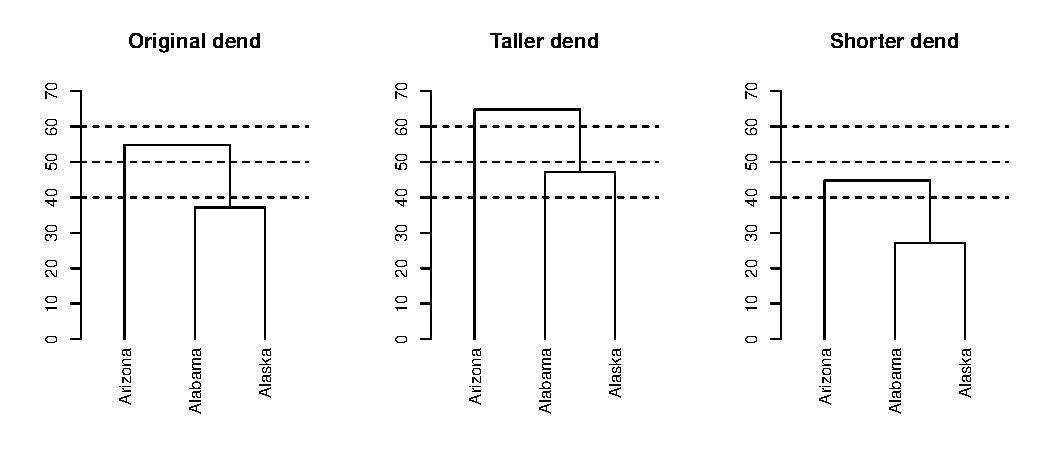
\includegraphics[width=\maxwidth]{figure/unnamed-chunk-23} 

}



\end{knitrout}




Sometimes we wish to "unbranch" the dendrogram, meaning that we merge one of the tree's branches with its root. This is useful, for example, when merging phylogenetic trees from several families, and being unwilling to assume a specific root/height to the merged trees. unbranching can be done using the \code{unbranch} (S3) function (notice the use of the \code{branch_becoming_root} parameter):


\begin{knitrout}
\definecolor{shadecolor}{rgb}{0.969, 0.969, 0.969}\color{fgcolor}\begin{kframe}
\begin{alltt}
\hlstd{hc} \hlkwb{<-} \hlkwd{hclust}\hlstd{(}\hlkwd{dist}\hlstd{(USArrests[}\hlnum{10}\hlopt{:}\hlnum{13}\hlstd{, ]),} \hlstr{"ward"}\hlstd{)}
\hlstd{dend} \hlkwb{<-} \hlkwd{as.dendrogram}\hlstd{(hc}\hlstd{)}

\hlstd{unbranched_dend} \hlkwb{<-} \hlkwd{unbranch}\hlstd{(dend,} \hlkwc{branch_becoming_root} \hlstd{=} \hlnum{1}\hlstd{)}
\hlstd{unbranched_dend_2} \hlkwb{<-} \hlkwd{unbranch}\hlstd{(unbranched_dend,} \hlkwc{branch_becoming_root} \hlstd{=} \hlnum{3}\hlstd{)}

\hlkwd{par}\hlstd{(}\hlkwc{mfrow} \hlstd{=} \hlkwd{c}\hlstd{(}\hlnum{1}\hlstd{,} \hlnum{3}\hlstd{))}
\hlkwd{plot}\hlstd{(dend)}
\hlkwd{plot}\hlstd{(unbranched_dend)}
\hlkwd{plot}\hlstd{(unbranched_dend_2)}
\end{alltt}
\end{kframe}

{\centering 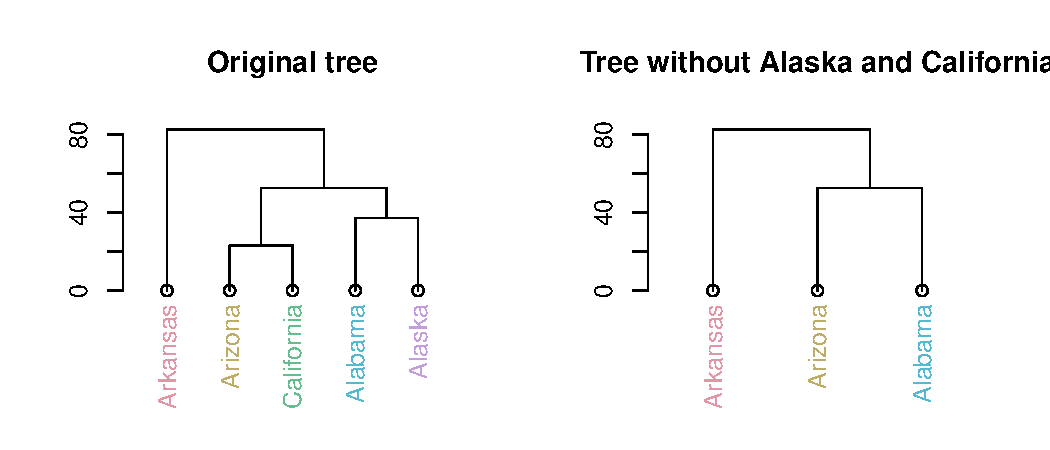
\includegraphics[width=\maxwidth]{figure/unnamed-chunk-24} 

}



\end{knitrout}


While the \code{unbranch.hclust} method exists, it is not expected to work since \code{hclust} objects are not designed to handle non-binary trees (hence the advantage of using \code{dendrogram} objects). For \code{phylo} objects (from the \pkg{ape} package), there is also a method that would simply use \code{ape:::unbranch(phy = x)}.

In some rare cases, we might wish to equalize the heights of root's branches. For this we can use the \code{flatten.dendrogram} function:


\begin{knitrout}
\definecolor{shadecolor}{rgb}{0.969, 0.969, 0.969}\color{fgcolor}\begin{kframe}
\begin{alltt}
\hlstd{hc} \hlkwb{<-} \hlkwd{hclust}\hlstd{(}\hlkwd{dist}\hlstd{(USArrests[}\hlnum{10}\hlopt{:}\hlnum{13}\hlstd{, ]),} \hlstr{"ward"}\hlstd{)}
\hlstd{dend} \hlkwb{<-} \hlkwd{as.dendrogram}\hlstd{(hc}\hlstd{)}

\hlstd{flatten_dend_1} \hlkwb{<-} \hlkwd{flatten.dendrogram}\hlstd{(dend,} \hlkwc{FUN} \hlstd{= max)}
\hlstd{flatten_dend_2} \hlkwb{<-} \hlkwd{flatten.dendrogram}\hlstd{(dend,} \hlkwc{FUN} \hlstd{= min}\hlstd{)}

\hlkwd{par}\hlstd{(}\hlkwc{mfrow} \hlstd{=} \hlkwd{c}\hlstd{(}\hlnum{1}\hlstd{,} \hlnum{3}\hlstd{))}
\hlkwd{plot}\hlstd{(dend,} \hlkwc{main} \hlstd{=} \hlstr{"Original tree"}\hlstd{)}
\hlkwd{abline}\hlstd{(}\hlkwc{h} \hlstd{=} \hlkwd{c}\hlstd{(}\hlnum{50}\hlstd{,} \hlnum{100}\hlstd{),} \hlkwc{lty} \hlstd{=} \hlnum{2}\hlstd{)}
\hlkwd{plot}\hlstd{(flatten_dend_1,} \hlkwc{main} \hlstd{=} \hlstr{"Flatten tree \textbackslash{}n(max branches height)"}\hlstd{)}
\hlkwd{abline}\hlstd{(}\hlkwc{h} \hlstd{=} \hlkwd{c}\hlstd{(}\hlnum{50}\hlstd{,} \hlnum{100}\hlstd{),} \hlkwc{lty} \hlstd{=} \hlnum{2}\hlstd{)}
\hlkwd{plot}\hlstd{(flatten_dend_2,} \hlkwc{main} \hlstd{=} \hlstr{"Flatten tree \textbackslash{}n(min branches height)"}\hlstd{)}
\hlkwd{abline}\hlstd{(}\hlkwc{h} \hlstd{=} \hlkwd{c}\hlstd{(}\hlnum{50}\hlstd{,} \hlnum{100}\hlstd{),} \hlkwc{lty} \hlstd{=} \hlnum{2}\hlstd{)}
\end{alltt}
\end{kframe}

{\centering 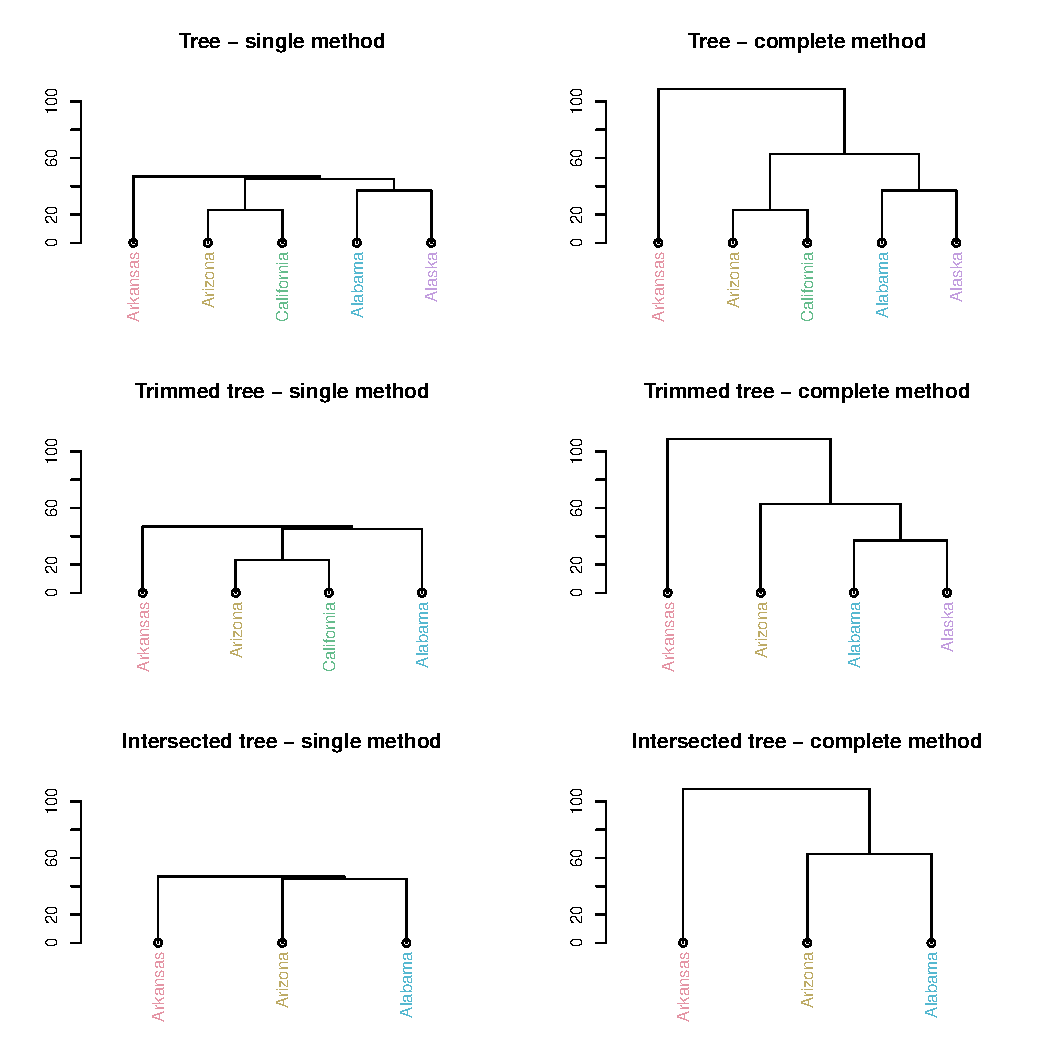
\includegraphics[width=\maxwidth]{figure/unnamed-chunk-25} 

}



\end{knitrout}





\subsection{Coloring labels of leaves}

Coloring labels can sometimes be useful, it is done through the \code{labels_colors} function (which also has assignemnt). Notice the assignment recycling, as well as the differene in the appearence of a dot when labels' color is black, compared to when it is NULL:

\begin{knitrout}
\definecolor{shadecolor}{rgb}{0.969, 0.969, 0.969}\color{fgcolor}\begin{kframe}
\begin{alltt}
\hlkwd{par}\hlstd{(}\hlkwc{mfrow} \hlstd{=} \hlkwd{c}\hlstd{(}\hlnum{1}\hlstd{,} \hlnum{3}\hlstd{)}\hlstd{)}

\hlstd{hc} \hlkwb{<-} \hlkwd{hclust}\hlstd{(}\hlkwd{dist}\hlstd{(USArrests[}\hlnum{1}\hlopt{:}\hlnum{3}\hlstd{, ]),} \hlstr{"ave"}\hlstd{)}
\hlstd{dend} \hlkwb{<-} \hlkwd{as.dendrogram}\hlstd{(hc}\hlstd{)}

\hlcom{# Defaults:}
\hlkwd{labels_colors}\hlstd{(dend)}
\end{alltt}
\begin{verbatim}
## NULL
\end{verbatim}
\begin{alltt}
\hlkwd{plot}\hlstd{(dend}\hlstd{)}

\hlcom{# let's add some color:}
\hlkwd{require}\hlstd{(colorspace)}
\hlkwd{labels_colors}\hlstd{(dend)} \hlkwb{<-} \hlkwd{rainbow_hcl}\hlstd{(}\hlnum{3}\hlstd{)}
\hlkwd{labels_colors}\hlstd{(dend)}
\end{alltt}
\begin{verbatim}
##   Arizona   Alabama    Alaska 
## "#E495A5" "#86B875" "#7DB0DD"
\end{verbatim}
\begin{alltt}
\hlkwd{plot}\hlstd{(dend}\hlstd{)}

\hlcom{# changing color to black}
\hlkwd{labels_colors}\hlstd{(dend)} \hlkwb{<-} \hlnum{1}
\end{alltt}


{\ttfamily\noindent\color{warningcolor}{\#\# Warning: Length of color vector was shorter than the number of leaves - vector color recycled}}\begin{alltt}
\hlkwd{labels_colors}\hlstd{(dend)}
\end{alltt}
\begin{verbatim}
## Arizona Alabama  Alaska 
##       1       1       1
\end{verbatim}
\begin{alltt}
\hlkwd{plot}\hlstd{(dend)}
\end{alltt}
\end{kframe}

{\centering 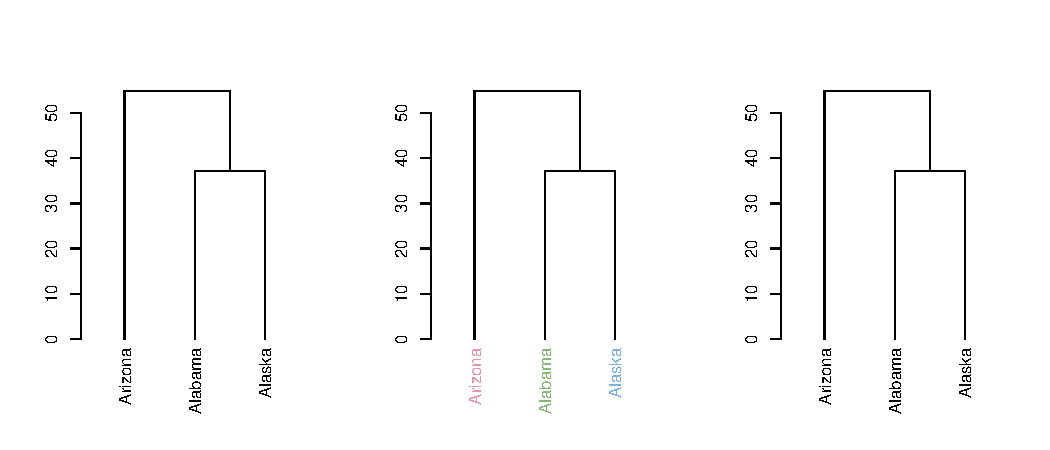
\includegraphics[width=\maxwidth]{figure/unnamed-chunk-26} 

}


\begin{kframe}\begin{alltt}
\hlcom{# removing color (and the nodePar completely - if it has no}
\hlcom{# other attributed but lab.col)}
\hlkwd{labels_colors}\hlstd{(dend)} \hlkwb{<-} \hlkwa{NULL}
\end{alltt}


{\ttfamily\noindent\color{warningcolor}{\#\# Warning: Length of color vector was shorter than the number of leaves - vector color recycled\\\#\# Warning: 'x' is NULL so the result will be NULL}}\begin{alltt}
\hlkwd{labels_colors}\hlstd{(dend)}
\end{alltt}
\begin{verbatim}
## NULL
\end{verbatim}
\end{kframe}
\end{knitrout}





\subsection{Hanging a dendrogram}

Hanging a tree means that we change the height of the leaves to be near their parent node. Hanging helps when examining the toplogy of the tree. Currently, hanging of a dendrogram was possible by going through the hclust object, but now you can simply use the \code{hang.dendrogram} function. Here is an example:


\begin{knitrout}
\definecolor{shadecolor}{rgb}{0.969, 0.969, 0.969}\color{fgcolor}\begin{kframe}
\begin{alltt}
\hlstd{hc} \hlkwb{<-} \hlkwd{hclust}\hlstd{(}\hlkwd{dist}\hlstd{(USArrests[}\hlnum{1}\hlopt{:}\hlnum{9}\hlstd{, ]),} \hlstr{"ave"}\hlstd{)}
\hlstd{dend} \hlkwb{<-} \hlkwd{as.dendrogram}\hlstd{(hc)}
\hlstd{hang_dend_1} \hlkwb{<-} \hlkwd{hang.dendrogram}\hlstd{(dend,} \hlkwc{hang} \hlstd{=} \hlnum{0.1}\hlstd{)}
\hlstd{hang_dend_2} \hlkwb{<-} \hlkwd{as.dendrogram}\hlstd{(hc,} \hlkwc{hang} \hlstd{=} \hlnum{0.1}\hlstd{)}  \hlcom{# another way of doing it, if }
\hlcom{# we could move from/to hclust}
\hlkwd{identical}\hlstd{(hang_dend_1, hang_dend_2)}  \hlcom{# and they are the same :)}
\end{alltt}
\begin{verbatim}
## [1] TRUE
\end{verbatim}
\begin{alltt}
\hlkwd{require}\hlstd{(colorspace)}
\hlkwd{labels_colors}\hlstd{(hang_dend_1)} \hlkwb{<-} \hlkwd{rainbow_hcl}\hlstd{(}\hlkwd{nleaves}\hlstd{(hang_dend_1)}\hlstd{)}

\hlkwd{par}\hlstd{(}\hlkwc{mfrow} \hlstd{=} \hlkwd{c}\hlstd{(}\hlnum{1}\hlstd{,} \hlnum{2}\hlstd{))}
\hlkwd{plot}\hlstd{(hc,} \hlkwc{main} \hlstd{=} \hlstr{"Hanged hclust tree"}\hlstd{)}
\hlkwd{plot}\hlstd{(hang_dend_1,} \hlkwc{main} \hlstd{=} \hlstr{"Hanged dendrogram tree"}\hlstd{)}
\end{alltt}
\end{kframe}

{\centering 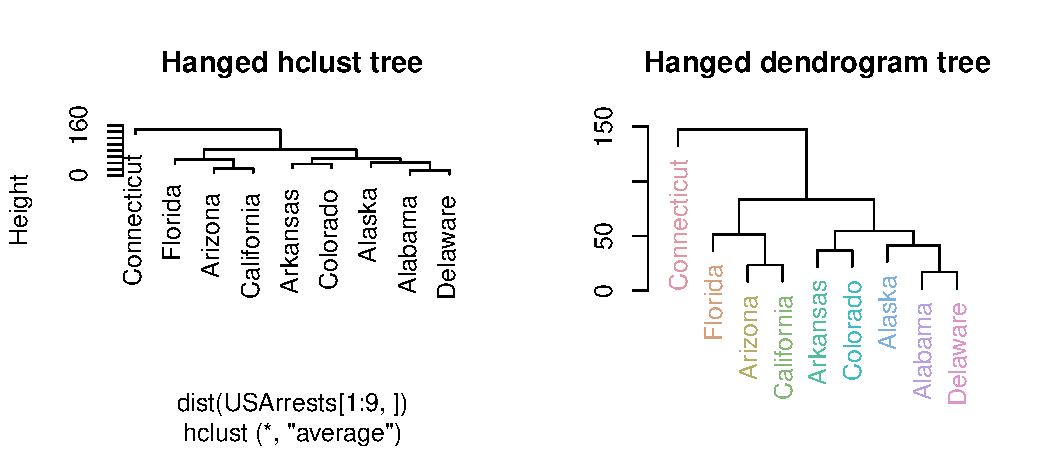
\includegraphics[width=\maxwidth]{figure/unnamed-chunk-27} 

}



\end{knitrout}




\subsection{Trimming leaves}

Trimming a tree from some leaves can be done using the \code{prune} (S3 method) function (notice that the attributes of the pruned tree are updated):

\begin{knitrout}
\definecolor{shadecolor}{rgb}{0.969, 0.969, 0.969}\color{fgcolor}\begin{kframe}
\begin{alltt}
\hlstd{hc} \hlkwb{<-} \hlkwd{hclust}\hlstd{(}\hlkwd{dist}\hlstd{(USArrests[}\hlnum{1}\hlopt{:}\hlnum{5}\hlstd{, ]),} \hlstr{"ave"}\hlstd{)}
\hlstd{dend} \hlkwb{<-} \hlkwd{as.dendrogram}\hlstd{(hc)}
\hlkwd{library}\hlstd{(colorspace)}
\hlkwd{labels_colors}\hlstd{(dend)} \hlkwb{<-} \hlkwd{rainbow_hcl}\hlstd{(}\hlnum{5}\hlstd{)}

\hlstd{pruned_dend} \hlkwb{<-} \hlkwd{prune}\hlstd{(dend,} \hlkwd{c}\hlstd{(}\hlstr{"Alaska"}\hlstd{,} \hlstr{"California"}\hlstd{)}\hlstd{)}

\hlkwd{str}\hlstd{(}\hlkwd{unclass}\hlstd{(pruned_dend))}
\end{alltt}
\begin{verbatim}
## List of 2
##  $ : atomic [1:1] 4
##   ..- attr(*, "members")= int 1
##   ..- attr(*, "height")= num 0
##   ..- attr(*, "label")= chr "Arkansas"
##   ..- attr(*, "leaf")= logi TRUE
##   ..- attr(*, "nodePar")=List of 2
##   .. ..$ lab.col: chr "#E495A5"
##   .. ..$ pch    : logi NA
##  $ :List of 2
##   ..$ : atomic [1:1] 3
##   .. ..- attr(*, "label")= chr "Arizona"
##   .. ..- attr(*, "members")= int 1
##   .. ..- attr(*, "height")= num 0
##   .. ..- attr(*, "leaf")= logi TRUE
##   .. ..- attr(*, "nodePar")=List of 2
##   .. .. ..$ lab.col: chr "#BDAB66"
##   .. .. ..$ pch    : logi NA
##   ..$ : atomic [1:1] 1
##   .. ..- attr(*, "label")= chr "Alabama"
##   .. ..- attr(*, "members")= int 1
##   .. ..- attr(*, "height")= num 0
##   .. ..- attr(*, "leaf")= logi TRUE
##   .. ..- attr(*, "nodePar")=List of 2
##   .. .. ..$ lab.col: chr "#55B8D0"
##   .. .. ..$ pch    : logi NA
##   ..- attr(*, "members")= num 2
##   ..- attr(*, "midpoint")= num 0.5
##   ..- attr(*, "height")= num 52.6
##  - attr(*, "members")= num 3
##  - attr(*, "midpoint")= num 0.75
##  - attr(*, "height")= num 82.6
\end{verbatim}
\begin{alltt}
\hlkwd{par}\hlstd{(}\hlkwc{mfrow} \hlstd{=} \hlkwd{c}\hlstd{(}\hlnum{1}\hlstd{,} \hlnum{2}\hlstd{))}
\hlkwd{plot}\hlstd{(dend,} \hlkwc{main} \hlstd{=} \hlstr{"Original tree"}\hlstd{)}
\hlkwd{plot}\hlstd{(pruned_dend,} \hlkwc{main} \hlstd{=} \hlstr{"Tree without Alaska and California"}\hlstd{)}
\end{alltt}
\end{kframe}

{\centering 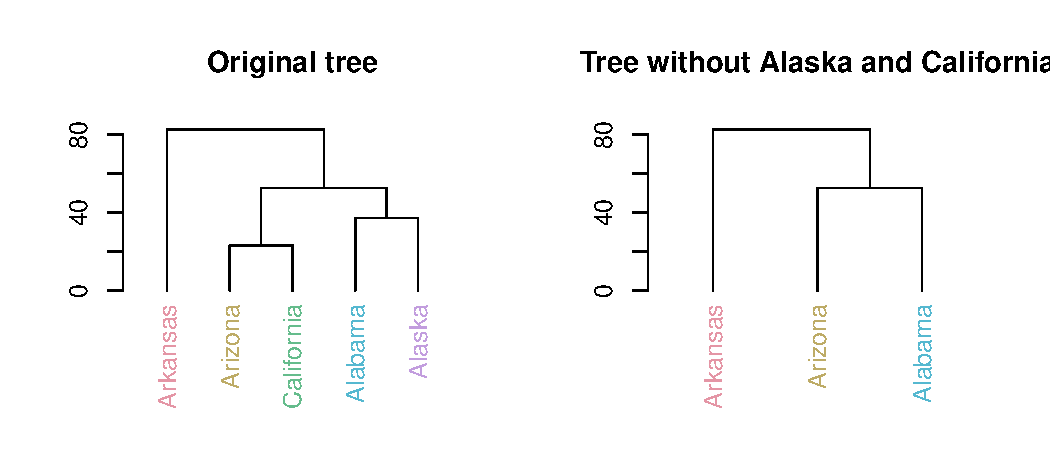
\includegraphics[width=\maxwidth]{figure/unnamed-chunk-28} 

}



\end{knitrout}


If we have two trees, we can use the \code{intersect_trees} function to reduce both trees to have the same labels (this will be useful later when we'd like to compare the two trees):


\begin{knitrout}
\definecolor{shadecolor}{rgb}{0.969, 0.969, 0.969}\color{fgcolor}\begin{kframe}
\begin{alltt}
\hlstd{hc_1} \hlkwb{<-} \hlkwd{hclust}\hlstd{(}\hlkwd{dist}\hlstd{(USArrests[}\hlnum{1}\hlopt{:}\hlnum{5}\hlstd{, ]),} \hlstr{"single"}\hlstd{)}
\hlstd{hc_2} \hlkwb{<-} \hlkwd{hclust}\hlstd{(}\hlkwd{dist}\hlstd{(USArrests[}\hlnum{1}\hlopt{:}\hlnum{5}\hlstd{, ]),} \hlstr{"complete"}\hlstd{)}
\hlstd{dend_1} \hlkwb{<-} \hlkwd{as.dendrogram}\hlstd{(hc_1)}
\hlstd{dend_2} \hlkwb{<-} \hlkwd{as.dendrogram}\hlstd{(hc_2}\hlstd{)}

\hlkwd{library}\hlstd{(colorspace)}
\hlkwd{labels_colors}\hlstd{(dend_1)} \hlkwb{<-} \hlkwd{rainbow_hcl}\hlstd{(}\hlnum{5}\hlstd{)}
\hlkwd{labels_colors}\hlstd{(dend_2)} \hlkwb{<-} \hlkwd{rainbow_hcl}\hlstd{(}\hlnum{5}\hlstd{)}


\hlstd{pruned_dend_1} \hlkwb{<-} \hlkwd{prune}\hlstd{(dend_1,} \hlkwd{c}\hlstd{(}\hlstr{"Alaska"}\hlstd{))}
\hlstd{pruned_dend_2} \hlkwb{<-} \hlkwd{prune}\hlstd{(dend_2,} \hlkwd{c}\hlstd{(}\hlstr{"California"}\hlstd{)}\hlstd{)}

\hlstd{dends_12} \hlkwb{<-} \hlkwd{intersect_trees}\hlstd{(pruned_dend_1, pruned_dend_2}\hlstd{)}

\hlkwd{par}\hlstd{(}\hlkwc{mfrow} \hlstd{=} \hlkwd{c}\hlstd{(}\hlnum{3}\hlstd{,} \hlnum{2}\hlstd{))}
\hlkwd{plot}\hlstd{(dend_1,} \hlkwc{main} \hlstd{=} \hlstr{"Tree - single method"}\hlstd{,} \hlkwc{ylim} \hlstd{=} \hlkwd{c}\hlstd{(}\hlnum{0}\hlstd{,} \hlnum{110}\hlstd{))}
\hlkwd{plot}\hlstd{(dend_2,} \hlkwc{main} \hlstd{=} \hlstr{"Tree - complete method"}\hlstd{,} \hlkwc{ylim} \hlstd{=} \hlkwd{c}\hlstd{(}\hlnum{0}\hlstd{,} \hlnum{110}\hlstd{))}
\hlkwd{plot}\hlstd{(pruned_dend_1,} \hlkwc{main} \hlstd{=} \hlstr{"Trimmed tree - single method"}\hlstd{,} \hlkwc{ylim} \hlstd{=} \hlkwd{c}\hlstd{(}\hlnum{0}\hlstd{,}
    \hlnum{110}\hlstd{))}
\hlkwd{plot}\hlstd{(pruned_dend_2,} \hlkwc{main} \hlstd{=} \hlstr{"Trimmed tree - complete method"}\hlstd{,}
    \hlkwc{ylim} \hlstd{=} \hlkwd{c}\hlstd{(}\hlnum{0}\hlstd{,} \hlnum{110}\hlstd{))}
\hlkwd{plot}\hlstd{(dends_12[[}\hlnum{1}\hlstd{]],} \hlkwc{main} \hlstd{=} \hlstr{"Intersected tree - single method"}\hlstd{,}
    \hlkwc{ylim} \hlstd{=} \hlkwd{c}\hlstd{(}\hlnum{0}\hlstd{,} \hlnum{110}\hlstd{))}
\hlkwd{plot}\hlstd{(dends_12[[}\hlnum{2}\hlstd{]],} \hlkwc{main} \hlstd{=} \hlstr{"Intersected tree - complete method"}\hlstd{,}
    \hlkwc{ylim} \hlstd{=} \hlkwd{c}\hlstd{(}\hlnum{0}\hlstd{,} \hlnum{110}\hlstd{))}
\end{alltt}
\end{kframe}

{\centering 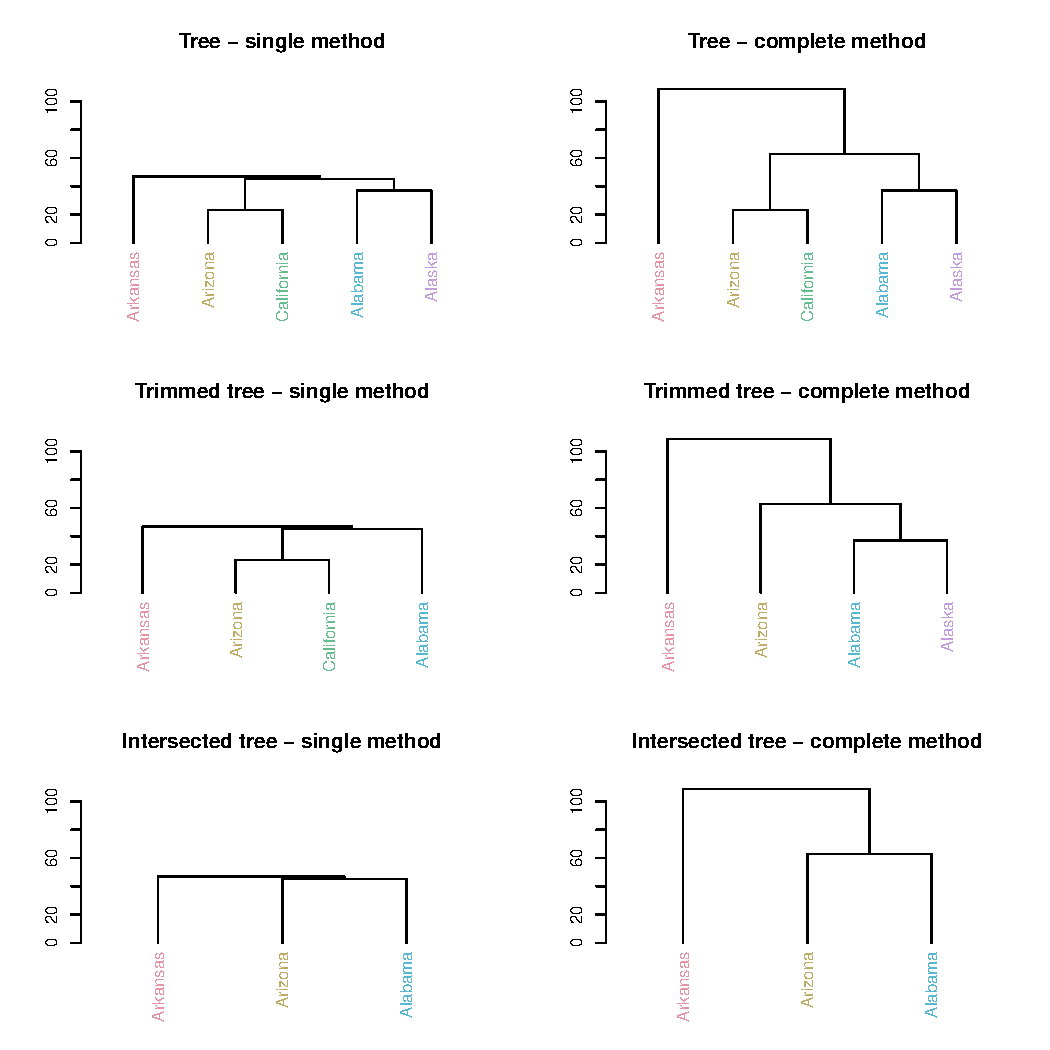
\includegraphics[width=\maxwidth]{figure/unnamed-chunk-29} 

}


\begin{kframe}\begin{alltt}


\end{alltt}
\end{kframe}
\end{knitrout}


Sidenote: a similar function, called \code{plotColoredClusters}, is available in the \pkg{ClassDiscovery} package for \code{hclust} objects.


\subsection{Rotating branches}

A dendrogram is an object which can be rotated on its hinges without 
changing its topological.

Rotating a dendrogram in base R can be done using the \code{reorder} function.
The problem with this function is that it is not very intuitive. For this reason
we wrote the \code{rotate} function. It has two main arguments: the object, and
the order we wish to rotate it by. The order parameter can be either a numeric
vector, used in a similar way we would order a simple character vector. Or, the
order parameter can also be a character vector of the labels of the tree, given
in the new desired order of the tree.

It is also worth noting that some order are impossible to achieve for a given 
tree's topology. In such a case, the function will do its "best" to get as close
as possible.

Here are a few examples:


\begin{knitrout}
\definecolor{shadecolor}{rgb}{0.969, 0.969, 0.969}\color{fgcolor}\begin{kframe}
\begin{alltt}
\hlstd{hc} \hlkwb{<-} \hlkwd{hclust}\hlstd{(}\hlkwd{dist}\hlstd{(USArrests[}\hlkwd{c}\hlstd{(}\hlnum{1}\hlstd{,} \hlnum{6}\hlstd{,} \hlnum{13}\hlstd{,} \hlnum{20}\hlstd{,} \hlnum{23}\hlstd{), ]),} \hlstr{"ave"}\hlstd{)}
\hlstd{dend} \hlkwb{<-} \hlkwd{as.dendrogram}\hlstd{(hc}\hlstd{)}

\hlcom{# For dendrogram objects:}
\hlkwd{require}\hlstd{(colorspace)}
\hlkwd{labels_colors}\hlstd{(dend)} \hlkwb{<-} \hlkwd{rainbow_hcl}\hlstd{(}\hlkwd{nleaves}\hlstd{(dend))}
\hlcom{# let's color the labels to make the followup of the rotation}
\hlcom{# easier}
\hlkwd{par}\hlstd{(}\hlkwc{mfrow} \hlstd{=} \hlkwd{c}\hlstd{(}\hlnum{2}\hlstd{,} \hlnum{2}\hlstd{))}
\hlkwd{plot}\hlstd{(dend,} \hlkwc{main} \hlstd{=} \hlstr{"Original tree"}\hlstd{)}
\hlkwd{plot}\hlstd{(}\hlkwd{rotate}\hlstd{(dend,} \hlkwd{c}\hlstd{(}\hlnum{2}\hlopt{:}\hlnum{5}\hlstd{,} \hlnum{1}\hlstd{)),} \hlkwc{main} \hlstd{=} \hlstr{"Rotates the left most leaf \textbackslash{}n into the right side of the tree"}\hlstd{)}
\hlkwd{plot}\hlstd{(dend,} \hlkwc{main} \hlstd{=} \hlstr{"Original tree"}\hlstd{)}
\hlkwd{plot}\hlstd{(}\hlkwd{sort}\hlstd{(dend),} \hlkwc{main} \hlstd{=} \hlstr{"Sorts the labels by alphabetical order \textbackslash{}n \textbackslash{}n     and rotates the tree to give the best fit possible"}\hlstd{)}
\end{alltt}
\end{kframe}

{\centering 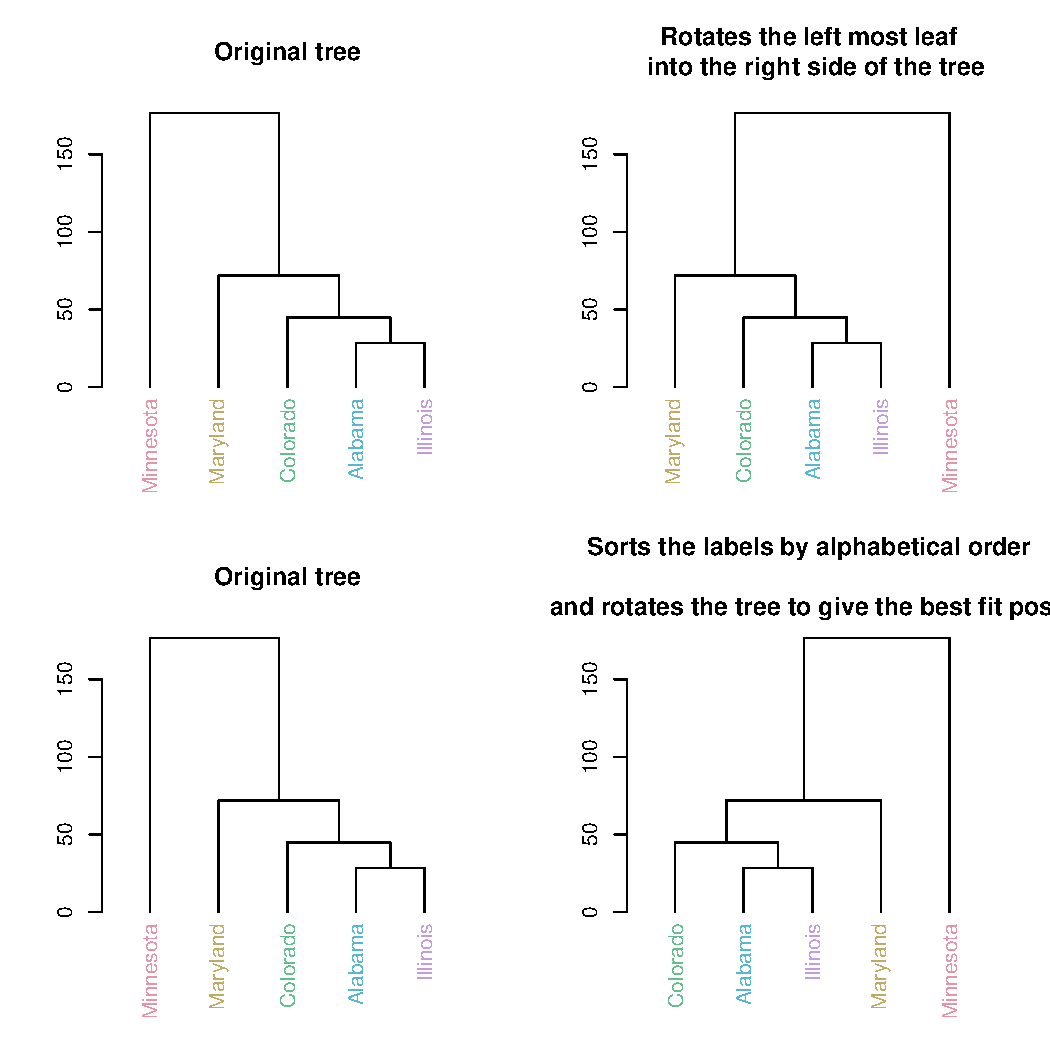
\includegraphics[width=\maxwidth]{figure/unnamed-chunk-30} 

}



\end{knitrout}





\subsection{Cutting trees}

The \code{hclust} function comes with a very powerfull \code{cutree} function, for extracting cluster grouping of the original data based on cutting the heirarchical tree at some height (or setting a predefined k - number of clusters). The limitation of this function is that it is only available for \code{hclust} object. Hence, if we are dealing with a tree which is NOT an ultrametric tree (e.g: ultrametric tree = a tree with monotone clustering heights), \code{cutree} would not be available for us (since \code{as.hclust} would not work on our dendrogram).

In \pkg{dendextend}, we extend \code{cutree} by turning it into an S3 method, with methods for dendrogram and phylo objects. The phylo method is only turning the phylo object to an hclust, and tries to work on it there. However, the dendrogram method (\code{cutree.dendrogram}) is a complete re-writing of \code{cutree} based on the \code{cut.dendrogram} function. \code{cutree.dendrogram} fully emulates \code{cutree} by default, but at the same time extends it with the type of trees it can handle, and with some other options.

Since \code{cutree.dendrogram} is written in \proglang{R}, it is slower than \code{cutree} which is implemented in \proglang{C}. If we can turn the dendrogram into hclust, we will use \code{cutree.hclust}, otherwise - \code{cutree.dendrogram} will be used.

Here are several examples of how these functions are used:

\begin{knitrout}
\definecolor{shadecolor}{rgb}{0.969, 0.969, 0.969}\color{fgcolor}\begin{kframe}
\begin{alltt}
\hlstd{hc} \hlkwb{<-} \hlkwd{hclust}\hlstd{(}\hlkwd{dist}\hlstd{(USArrests[}\hlkwd{c}\hlstd{(}\hlnum{1}\hlstd{,} \hlnum{6}\hlstd{,} \hlnum{13}\hlstd{,} \hlnum{20}\hlstd{,} \hlnum{23}\hlstd{), ]),} \hlstr{"ave"}\hlstd{)}
\hlstd{dend} \hlkwb{<-} \hlkwd{as.dendrogram}\hlstd{(hc)}
\hlstd{unbranch_dend} \hlkwb{<-} \hlkwd{unbranch}\hlstd{(dend,} \hlnum{2}\hlstd{)}

\hlkwd{cutree}\hlstd{(hc,} \hlkwc{k} \hlstd{=} \hlnum{2}\hlopt{:}\hlnum{4}\hlstd{)}  \hlcom{# on hclust}
\end{alltt}
\begin{verbatim}
##           2 3 4
## Alabama   1 1 1
## Colorado  1 1 2
## Illinois  1 1 1
## Maryland  1 2 3
## Minnesota 2 3 4
\end{verbatim}
\begin{alltt}
\hlkwd{cutree}\hlstd{(dend,} \hlkwc{k} \hlstd{=} \hlnum{2}\hlopt{:}\hlnum{4}\hlstd{)}  \hlcom{# on dendrogram}
\end{alltt}
\begin{verbatim}
##           2 3 4
## Alabama   1 1 1
## Colorado  1 1 2
## Illinois  1 1 1
## Maryland  1 2 3
## Minnesota 2 3 4
\end{verbatim}
\begin{alltt}
\hlkwd{cutree}\hlstd{(hc,} \hlkwc{k} \hlstd{=} \hlnum{2}\hlstd{)}  \hlcom{# on hclust}
\end{alltt}
\begin{verbatim}
##   Alabama  Colorado  Illinois  Maryland Minnesota 
##         1         1         1         1         2
\end{verbatim}
\begin{alltt}
\hlkwd{cutree}\hlstd{(dend,} \hlkwc{k} \hlstd{=} \hlnum{2}\hlstd{)}  \hlcom{# on dendrogram}
\end{alltt}
\begin{verbatim}
##   Alabama  Colorado  Illinois  Maryland Minnesota 
##         1         1         1         1         2
\end{verbatim}
\begin{alltt}
\hlkwd{cutree}\hlstd{(dend,} \hlkwc{h} \hlstd{=} \hlkwd{c}\hlstd{(}\hlnum{20}\hlstd{,} \hlnum{25.5}\hlstd{,} \hlnum{50}\hlstd{,} \hlnum{170}\hlstd{))}
\end{alltt}
\begin{verbatim}
##           20 25.5 50 170
## Alabama    1    1  1   1
## Colorado   2    2  1   1
## Illinois   3    3  1   1
## Maryland   4    4  2   1
## Minnesota  5    5  3   2
\end{verbatim}
\begin{alltt}
\hlkwd{cutree}\hlstd{(hc,} \hlkwc{h} \hlstd{=} \hlkwd{c}\hlstd{(}\hlnum{20}\hlstd{,} \hlnum{25.5}\hlstd{,} \hlnum{50}\hlstd{,} \hlnum{170}\hlstd{))}
\end{alltt}
\begin{verbatim}
##           20 25.5 50 170
## Alabama    1    1  1   1
## Colorado   2    2  1   1
## Illinois   3    3  1   1
## Maryland   4    4  2   1
## Minnesota  5    5  3   2
\end{verbatim}
\begin{alltt}
\hlcom{# the default (ordered by original data's order)}
\hlkwd{cutree}\hlstd{(dend,} \hlkwc{k} \hlstd{=} \hlnum{2}\hlopt{:}\hlnum{3}\hlstd{,} \hlkwc{order_clusters_as_data} \hlstd{=} \hlnum{FALSE}\hlstd{)}
\end{alltt}
\begin{verbatim}
## [1] 2 1 1 1 1
\end{verbatim}
\begin{alltt}
\hlkwd{labels}\hlstd{(dend)}
\end{alltt}
\begin{verbatim}
## [1] "Minnesota" "Maryland"  "Colorado"  "Alabama"  
## [5] "Illinois"
\end{verbatim}
\begin{alltt}
\hlcom{# cutree now works for unbranched trees!}
\hlcom{# as.hclust(unbranch_dend) # ERROR - can not do this...}
\hlkwd{cutree}\hlstd{(unbranch_dend,} \hlkwc{k} \hlstd{=} \hlnum{2}\hlstd{)}  \hlcom{# all NA's}
\end{alltt}


{\ttfamily\noindent\color{warningcolor}{\#\# Warning: Couldn't cut the tree - returning NA.\\\#\# Warning: You (probably) have some branches with equal heights so that there exist no height(h) that can create 2\ \ clusters}}\begin{verbatim}
## [1] NA NA NA NA NA
\end{verbatim}
\begin{alltt}
\hlkwd{cutree}\hlstd{(unbranch_dend,} \hlkwc{k} \hlstd{=} \hlnum{1}\hlopt{:}\hlnum{4}\hlstd{)}
\end{alltt}


{\ttfamily\noindent\color{warningcolor}{\#\# Warning: Couldn't cut the tree - returning NA.\\\#\# Warning: You (probably) have some branches with equal heights so that there exist no height(h) that can create 2\ \ clusters}}\begin{verbatim}
##           1  2 3 4
## Alabama   1 NA 2 2
## Colorado  1 NA 2 3
## Illinois  1 NA 2 2
## Maryland  1 NA 3 4
## Minnesota 1 NA 1 1
\end{verbatim}
\begin{alltt}
\hlkwd{cutree}\hlstd{(unbranch_dend,} \hlkwc{h} \hlstd{=} \hlkwd{c}\hlstd{(}\hlnum{20}\hlstd{,} \hlnum{25.5}\hlstd{,} \hlnum{50}\hlstd{,} \hlnum{170}\hlstd{))}
\end{alltt}
\begin{verbatim}
##           20 25.5 50 170
## Alabama    1    1  2   2
## Colorado   2    2  2   2
## Illinois   3    3  2   2
## Maryland   4    4  3   3
## Minnesota  5    5  1   1
\end{verbatim}
\begin{alltt}
\hlkwd{require}\hlstd{(microbenchmark)}
\hlcom{## this shows how as.hclust is expensive - but still worth it}
\hlcom{## if possible}
\hlkwd{microbenchmark}\hlstd{(}\hlkwd{cutree}\hlstd{(hc,} \hlkwc{k} \hlstd{=} \hlnum{2}\hlopt{:}\hlnum{4}\hlstd{),} \hlkwd{cutree}\hlstd{(}\hlkwd{as.hclust}\hlstd{(dend),} \hlkwc{k} \hlstd{=} \hlnum{2}\hlopt{:}\hlnum{4}\hlstd{),}
    \hlkwd{cutree}\hlstd{(dend,} \hlkwc{k} \hlstd{=} \hlnum{2}\hlopt{:}\hlnum{4}\hlstd{),} \hlkwd{cutree}\hlstd{(dend,} \hlkwc{k} \hlstd{=} \hlnum{2}\hlopt{:}\hlnum{4}\hlstd{,} \hlkwc{try_cutree_hclust} \hlstd{=} \hlnum{FALSE}\hlstd{))}
\end{alltt}
\begin{verbatim}
## Unit: microseconds
##                                              expr    min
##                               cutree(hc, k = 2:4)  136.6
##                  cutree(as.hclust(dend), k = 2:4) 1727.9
##                             cutree(dend, k = 2:4) 1825.9
##  cutree(dend, k = 2:4, try_cutree_hclust = FALSE) 8218.0
##      lq median     uq     max neval
##   142.2  145.6  194.6   324.8   100
##  1755.9 1834.9 1902.6  4882.0   100
##  1889.8 1945.5 1994.2  4950.9   100
##  8372.6 8512.6 8707.1 11539.5   100
\end{verbatim}
\begin{alltt}
\hlcom{# the dendrogram is MUCH slower...}


\hlcom{# and trying to 'hclust' is not expensive (which is nice...)}
\hlkwd{microbenchmark}\hlstd{(}\hlkwc{cutree_unbranch_dend} \hlstd{=} \hlkwd{cutree}\hlstd{(unbranch_dend,} \hlkwc{k} \hlstd{=} \hlnum{2}\hlopt{:}\hlnum{4}\hlstd{,}
    \hlkwc{warn} \hlstd{=} \hlnum{FALSE}\hlstd{),} \hlkwc{cutree_unbranch_dend_not_trying_to_hclust} \hlstd{=} \hlkwd{cutree}\hlstd{(unbranch_dend,}
    \hlkwc{k} \hlstd{=} \hlnum{2}\hlopt{:}\hlnum{4}\hlstd{,} \hlkwc{try_cutree_hclust} \hlstd{=} \hlnum{FALSE}\hlstd{,} \hlkwc{warn} \hlstd{=} \hlnum{FALSE}\hlstd{))}
\end{alltt}
\begin{verbatim}
## Unit: milliseconds
##                                       expr   min    lq
##                       cutree_unbranch_dend 6.691 6.784
##  cutree_unbranch_dend_not_trying_to_hclust 6.283 6.375
##  median    uq    max neval
##   6.894 7.052  9.978   100
##   6.488 6.679 13.087   100
\end{verbatim}
\begin{alltt}

\end{alltt}
\end{kframe}
\end{knitrout}



Having \code{cutree.dendrogram} available to us, we can now gain the ability to color branches for trees which can not be represented as an \code{hclust} object.

\subsection{Coloring branches}


Dendrogram plots with colored branches are used to easly distinguishing between different clusters on a tree. They have been available in R for many years in threads on the mailing lists and through various package. However, until recently, all of the functions in packages have always given the user a new \code{plot} function, without seperating the coloring of branches of a dendrogram from its plotting. Often the function for actually plotting the colored branched dendrogram would be hidden from the user. For example, the \pkg{labeltodendro} package \citep{CRAN:labeltodendro} gives a colored branch plot through the \code{colorplot} function, but the work horse for this is available in a hidden function called \code{dendroploth} or \code{dendroplotv}, both take care of the plotting by themselves (instead of modifying the dendrogram object, and then letting the base R function do the work). The same story happens in the \pkg{Heatplus} \citep{CRAN:Heatplus}, where the \code{plot.annHeatmap2} function actually uses the hidden function \code{cutplot.dendrogram} for doing the plotting.

This was changed in the beginning of 2013 thanks to Gregory Jefferis's \pkg{dendroextras} package \citep{CRAN:dendroextras}, which orgranized this through the \code{colour_clusters} function. In the \pkg{dendextend} package we imported his code into a new function called \code{color_branches}, with several useful modifications on the original code. The biggest limitation in the \code{colour_clusters} function is that it relies on changing the \code{dendrogram} into \code{hclust} in order to use \code{cutree} on it and get the clusters. This has the advantage of being fast, but the \textbf{disadvantage} of restricting the function to ultrametric and binary trees (the type of tree \code{hclust} objects can handle). In our implementation we implemented a new function called \code{cutree.dendrogram} (available through an S3 method), which can either relly on \code{hclust} for speed, but in case it is not possible will revert to find the clustering on the dendrogram object itself (the function is completely compatible with the base R \code{cutree} function). Also, our implementation of the \code{color_branches} function allows for repeated-multilayered coloring the branches. Another potential bug which is avoided in our implementation is to handle cases where the labels of the tree are of type Integer instead of Character (this happens if the \code{dendrogram} came from an \code{hclust}, used on the \code{dist} of data that has no \code{rownames}).

Here is an example of using \code{color_branches} combined with \code{labels_colors}:

\begin{knitrout}
\definecolor{shadecolor}{rgb}{0.969, 0.969, 0.969}\color{fgcolor}\begin{kframe}
\begin{alltt}
\hlkwd{require}\hlstd{(colorspace}\hlstd{)}

\hlkwd{data}\hlstd{(iris)}
\hlstd{d_iris} \hlkwb{<-} \hlkwd{dist}\hlstd{(iris[,} \hlopt{-}\hlnum{5}\hlstd{])}  \hlcom{# method='man' # is a bit better}
\hlstd{hc_iris} \hlkwb{<-} \hlkwd{hclust}\hlstd{(d_iris)}
\hlkwd{labels}\hlstd{(hc_iris)}  \hlcom{# no labels, because 'iris' has no row names}
\end{alltt}
\begin{verbatim}
## character(0)
\end{verbatim}
\begin{alltt}
\hlstd{dend_iris} \hlkwb{<-} \hlkwd{as.dendrogram}\hlstd{(hc_iris)}
\hlkwd{is.integer}\hlstd{(}\hlkwd{labels}\hlstd{(dend_iris))}  \hlcom{# this could cause problems...}
\end{alltt}
\begin{verbatim}
## [1] TRUE
\end{verbatim}
\begin{alltt}
\hlstd{iris_species} \hlkwb{<-} \hlkwd{rev}\hlstd{(}\hlkwd{levels}\hlstd{(iris[,} \hlnum{5}\hlstd{]))}
\hlstd{dend_iris} \hlkwb{<-} \hlkwd{color_branches}\hlstd{(dend_iris,} \hlkwc{k} \hlstd{=} \hlnum{3}\hlstd{,} \hlkwc{groupLabels} \hlstd{= iris_species)}
\hlkwd{is.character}\hlstd{(}\hlkwd{labels}\hlstd{(dend_iris))}  \hlcom{# labels are no longer 'integer'}
\end{alltt}
\begin{verbatim}
## [1] TRUE
\end{verbatim}
\begin{alltt}
\hlcom{# have the labels match the real classification of the}
\hlcom{# flowers:}
\hlkwd{labels_colors}\hlstd{(dend_iris)} \hlkwb{<-} \hlkwd{rainbow_hcl}\hlstd{(}\hlnum{3}\hlstd{)[}\hlkwd{sort_levels_values}\hlstd{(}\hlkwd{as.numeric}\hlstd{(iris[,}
    \hlnum{5}\hlstd{])[}\hlkwd{order.dendrogram}\hlstd{(dend_iris)])}\hlstd{]}

\hlcom{# We'll add the flower type}
\hlkwd{labels}\hlstd{(dend_iris)} \hlkwb{<-} \hlkwd{paste}\hlstd{(}\hlkwd{as.character}\hlstd{(iris[,} \hlnum{5}\hlstd{])[}\hlkwd{order.dendrogram}\hlstd{(dend_iris)],}
    \hlstr{"("}\hlstd{,} \hlkwd{labels}\hlstd{(dend_iris),} \hlstr{")"}\hlstd{,} \hlkwc{sep} \hlstd{=} \hlstr{""}\hlstd{)}

\hlstd{dend_iris} \hlkwb{<-} \hlkwd{hang.dendrogram}\hlstd{(dend_iris,} \hlkwc{hang_height} \hlstd{=} \hlnum{0.1}\hlstd{)}

\hlcom{# reduce the size of the labels:}
\hlstd{dend_iris} \hlkwb{<-} \hlkwd{assign_values_to_leaves_nodePar}\hlstd{(dend_iris,} \hlnum{0.5}\hlstd{,}
    \hlstr{"lab.cex"}\hlstd{)}
\end{alltt}


{\ttfamily\noindent\color{warningcolor}{\#\# Warning: Length of value vector was shorter than the number of leaves - vector value recycled}}\begin{alltt}
\hlkwd{par}\hlstd{(}\hlkwc{mar} \hlstd{=} \hlkwd{c}\hlstd{(}\hlnum{3}\hlstd{,} \hlnum{3}\hlstd{,} \hlnum{3}\hlstd{,} \hlnum{7}\hlstd{))}
\hlkwd{plot}\hlstd{(dend_iris,} \hlkwc{main} \hlstd{=} \hlstr{"Clustered Iris dataset\textbackslash{}n     (the labels give the true flower species)"}\hlstd{,}
    \hlkwc{horiz} \hlstd{=} \hlnum{TRUE}\hlstd{,} \hlkwc{nodePar} \hlstd{=} \hlkwd{list}\hlstd{(}\hlkwc{cex} \hlstd{=} \hlnum{0.007}\hlstd{))}
\hlkwd{legend}\hlstd{(}\hlstr{"topleft"}\hlstd{,} \hlkwc{legend} \hlstd{= iris_species,} \hlkwc{fill} \hlstd{=} \hlkwd{rainbow_hcl}\hlstd{(}\hlnum{3}\hlstd{))}
\end{alltt}
\end{kframe}

{\centering 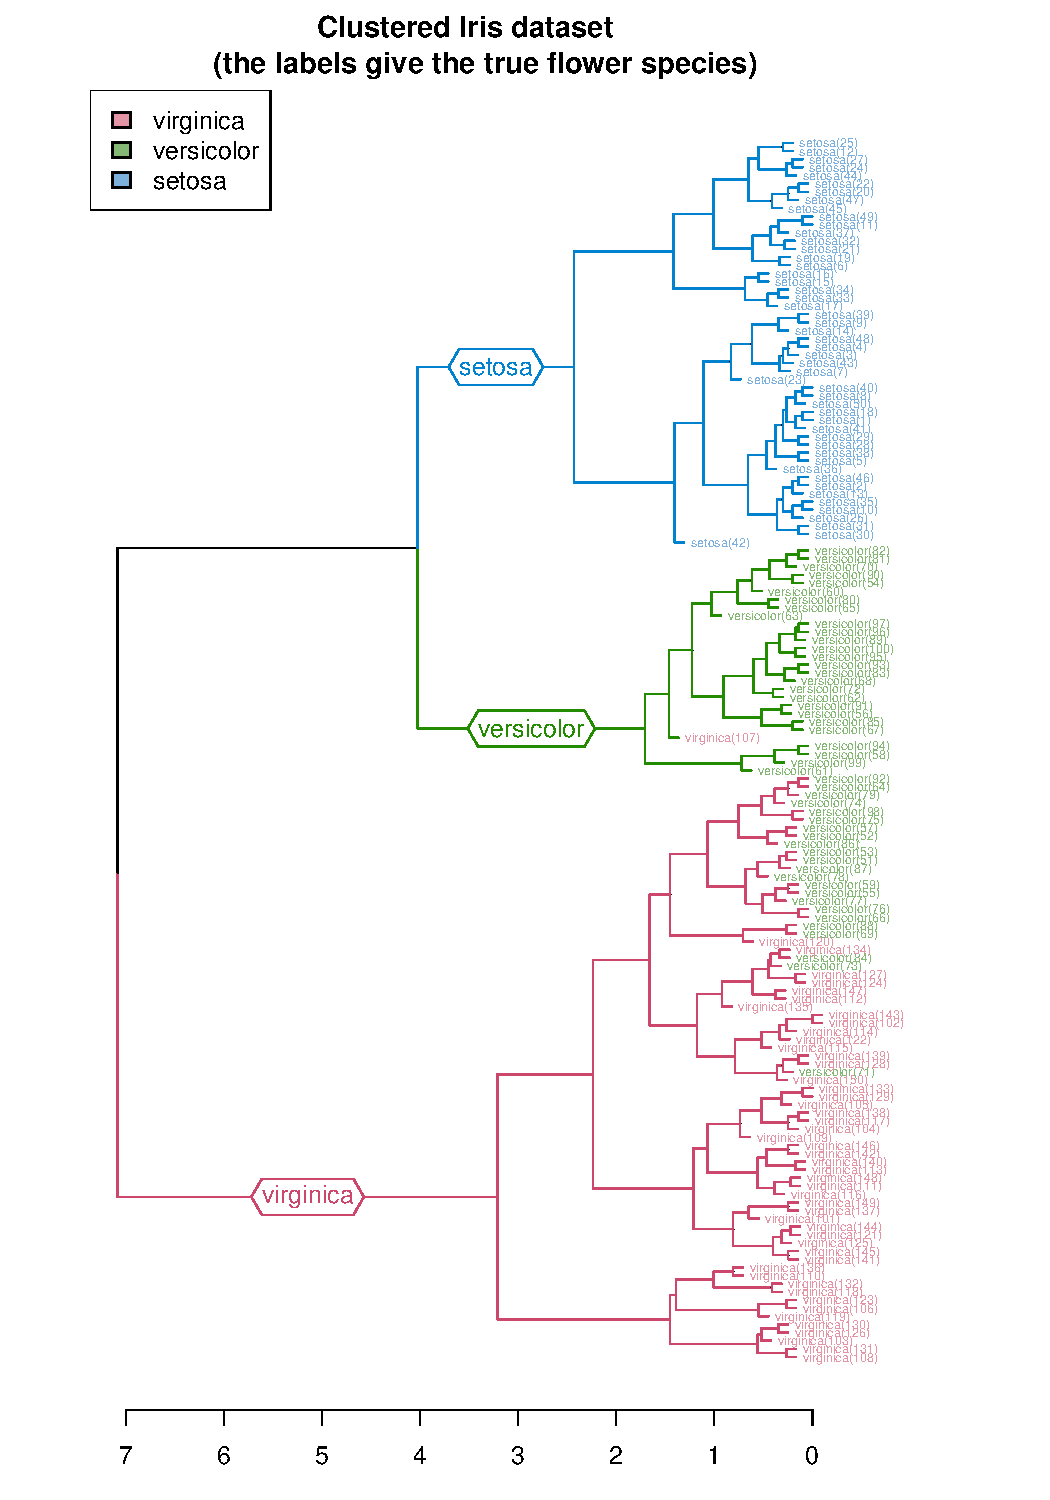
\includegraphics[width=\maxwidth]{figure/iris_colored_branches} 

}



\end{knitrout}


This simple visualization easily demonstrates how the seperation of the heirarchical clustering is very good with the "setosa" sepcies, but misses in labeling many "versicolor" species as "virginica".

The hanging of the tree also helps to locate extreme observations. For example, we can see that observation "virginica (107)" is not very similar to the Versicolor species, but still, it is amoung them. Also, "Versicolor (71)" is too much "within" the Virginica bush, and it is a wonder why that is.  Of course, the Iris dataset is very well known, and simpler pairs plot often help to locate such problems, yet - dendrogram trees (with all of their limitations) can help gain insights for very high-dimensional data where a simple pairs plot is not possible.

Here is the similar pairs plot. Notice the filled red and green dots, corrosponding with the extreme observations we have noticed in the dendrogram. Petal.Length vs Petal.Width gives the best example of why the green dot is an outlier. Whereas most plots show why the red dot is an outlier. There are of course other outliers, and a problem with classification, which we will not go futher into.

\begin{knitrout}
\definecolor{shadecolor}{rgb}{0.969, 0.969, 0.969}\color{fgcolor}\begin{kframe}
\begin{alltt}
\hlkwd{require}\hlstd{(colorspace}\hlstd{)}

\hlstd{species_col} \hlkwb{<-} \hlkwd{rev}\hlstd{(}\hlkwd{rainbow_hcl}\hlstd{(}\hlnum{3}\hlstd{))[}\hlkwd{as.numeric}\hlstd{(iris[,} \hlnum{5}\hlstd{])]}
\hlcom{# species_col[c(107,71)] <- 'red' # highlight the two extreme}
\hlcom{# cases we mentioned}
\hlstd{species_pch} \hlkwb{<-} \hlkwd{rep}\hlstd{(}\hlnum{1}\hlstd{,} \hlkwd{length}\hlstd{(species_col))}
\hlstd{species_pch[}\hlkwd{c}\hlstd{(}\hlnum{107}\hlstd{,} \hlnum{71}\hlstd{)]} \hlkwb{<-} \hlnum{19}  \hlcom{# highlight the two extreme cases we mentioned}

\hlkwd{pairs}\hlstd{(iris[,} \hlopt{-}\hlnum{5}\hlstd{],} \hlkwc{col} \hlstd{= species_col,} \hlkwc{pch} \hlstd{= species_pch)}
\end{alltt}
\end{kframe}

{\centering 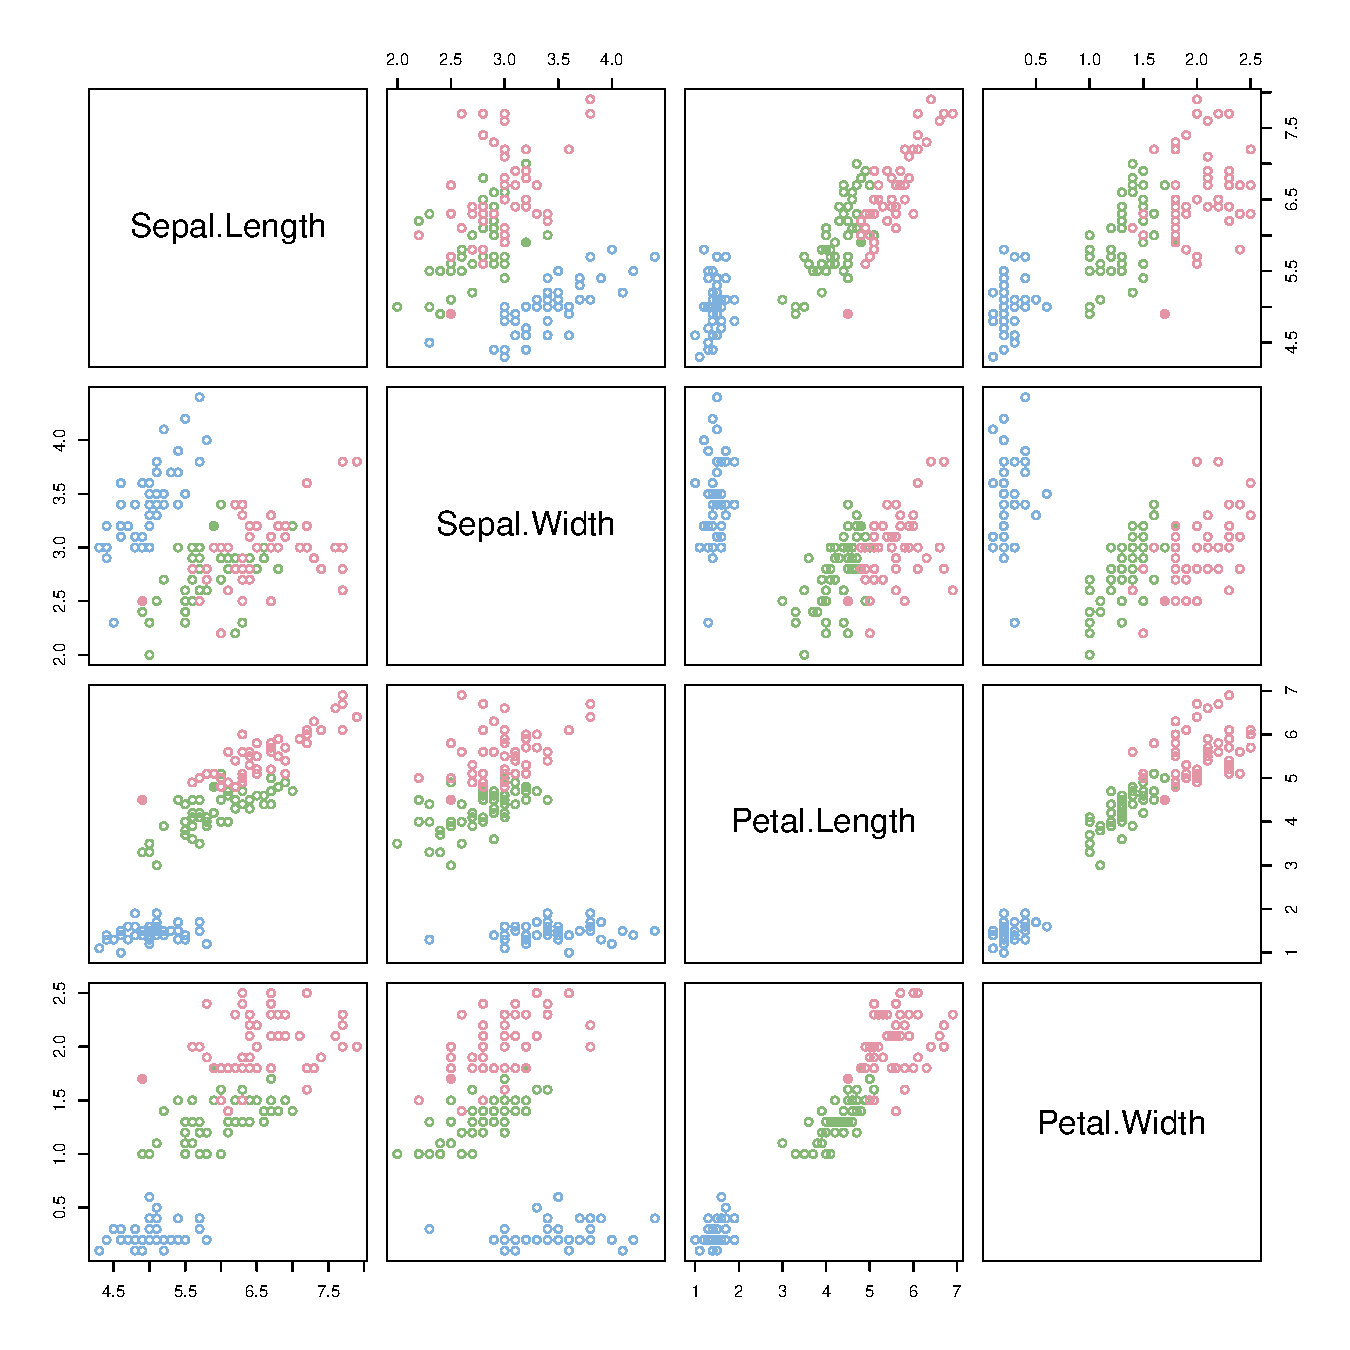
\includegraphics[width=\maxwidth]{figure/iris_colored_pairs_plot} 

}


\begin{kframe}\begin{alltt}

\end{alltt}
\end{kframe}
\end{knitrout}







\section{Tanglegrams - visually comparing two trees side-by-side}

\subsection{Tanglegram visualization}

A tanglegram plot gives two dendrogram (with the same set of labels), one facing the other, and having their labels connected by lines. Tanglegram can be used for visually comparing two methods of heirarchical clustering, and are sometimes used in biology when comparing two phylogenetic trees.

%% add references!

Here is an example of creating a tanglegram using \pkg{dendextend}:


\begin{knitrout}
\definecolor{shadecolor}{rgb}{0.969, 0.969, 0.969}\color{fgcolor}\begin{kframe}
\begin{alltt}
\hlstd{hc1} \hlkwb{<-} \hlkwd{hclust}\hlstd{(}\hlkwd{dist}\hlstd{(iris[,} \hlopt{-}\hlnum{5}\hlstd{]),} \hlstr{"com"}\hlstd{)}
\hlstd{hc2} \hlkwb{<-} \hlkwd{hclust}\hlstd{(}\hlkwd{dist}\hlstd{(iris[,} \hlopt{-}\hlnum{5}\hlstd{]),} \hlstr{"single"}\hlstd{)}
\hlstd{dend1} \hlkwb{<-} \hlkwd{as.dendrogram}\hlstd{(hc1)}
\hlstd{dend2} \hlkwb{<-} \hlkwd{as.dendrogram}\hlstd{(hc2)}
\hlkwd{tanglegram}\hlstd{(dend1, dend2,} \hlkwc{lab.cex} \hlstd{=} \hlnum{0.5}\hlstd{,} \hlkwc{edge.lwd} \hlstd{=} \hlnum{1}\hlstd{,} \hlkwc{margin_inner} \hlstd{=} \hlnum{3}\hlstd{,}
    \hlkwc{type} \hlstd{=} \hlstr{"r"}\hlstd{,} \hlkwc{center} \hlstd{=} \hlnum{TRUE}\hlstd{,} \hlkwc{k_branches} \hlstd{=} \hlnum{3}\hlstd{)}
\end{alltt}


{\ttfamily\noindent\color{warningcolor}{\#\# Warning: Length of value vector was shorter than the number of leaves - vector value recycled\\\#\# Warning: Length of value vector was shorter than the number of leaves - vector value recycled}}\end{kframe}

{\centering 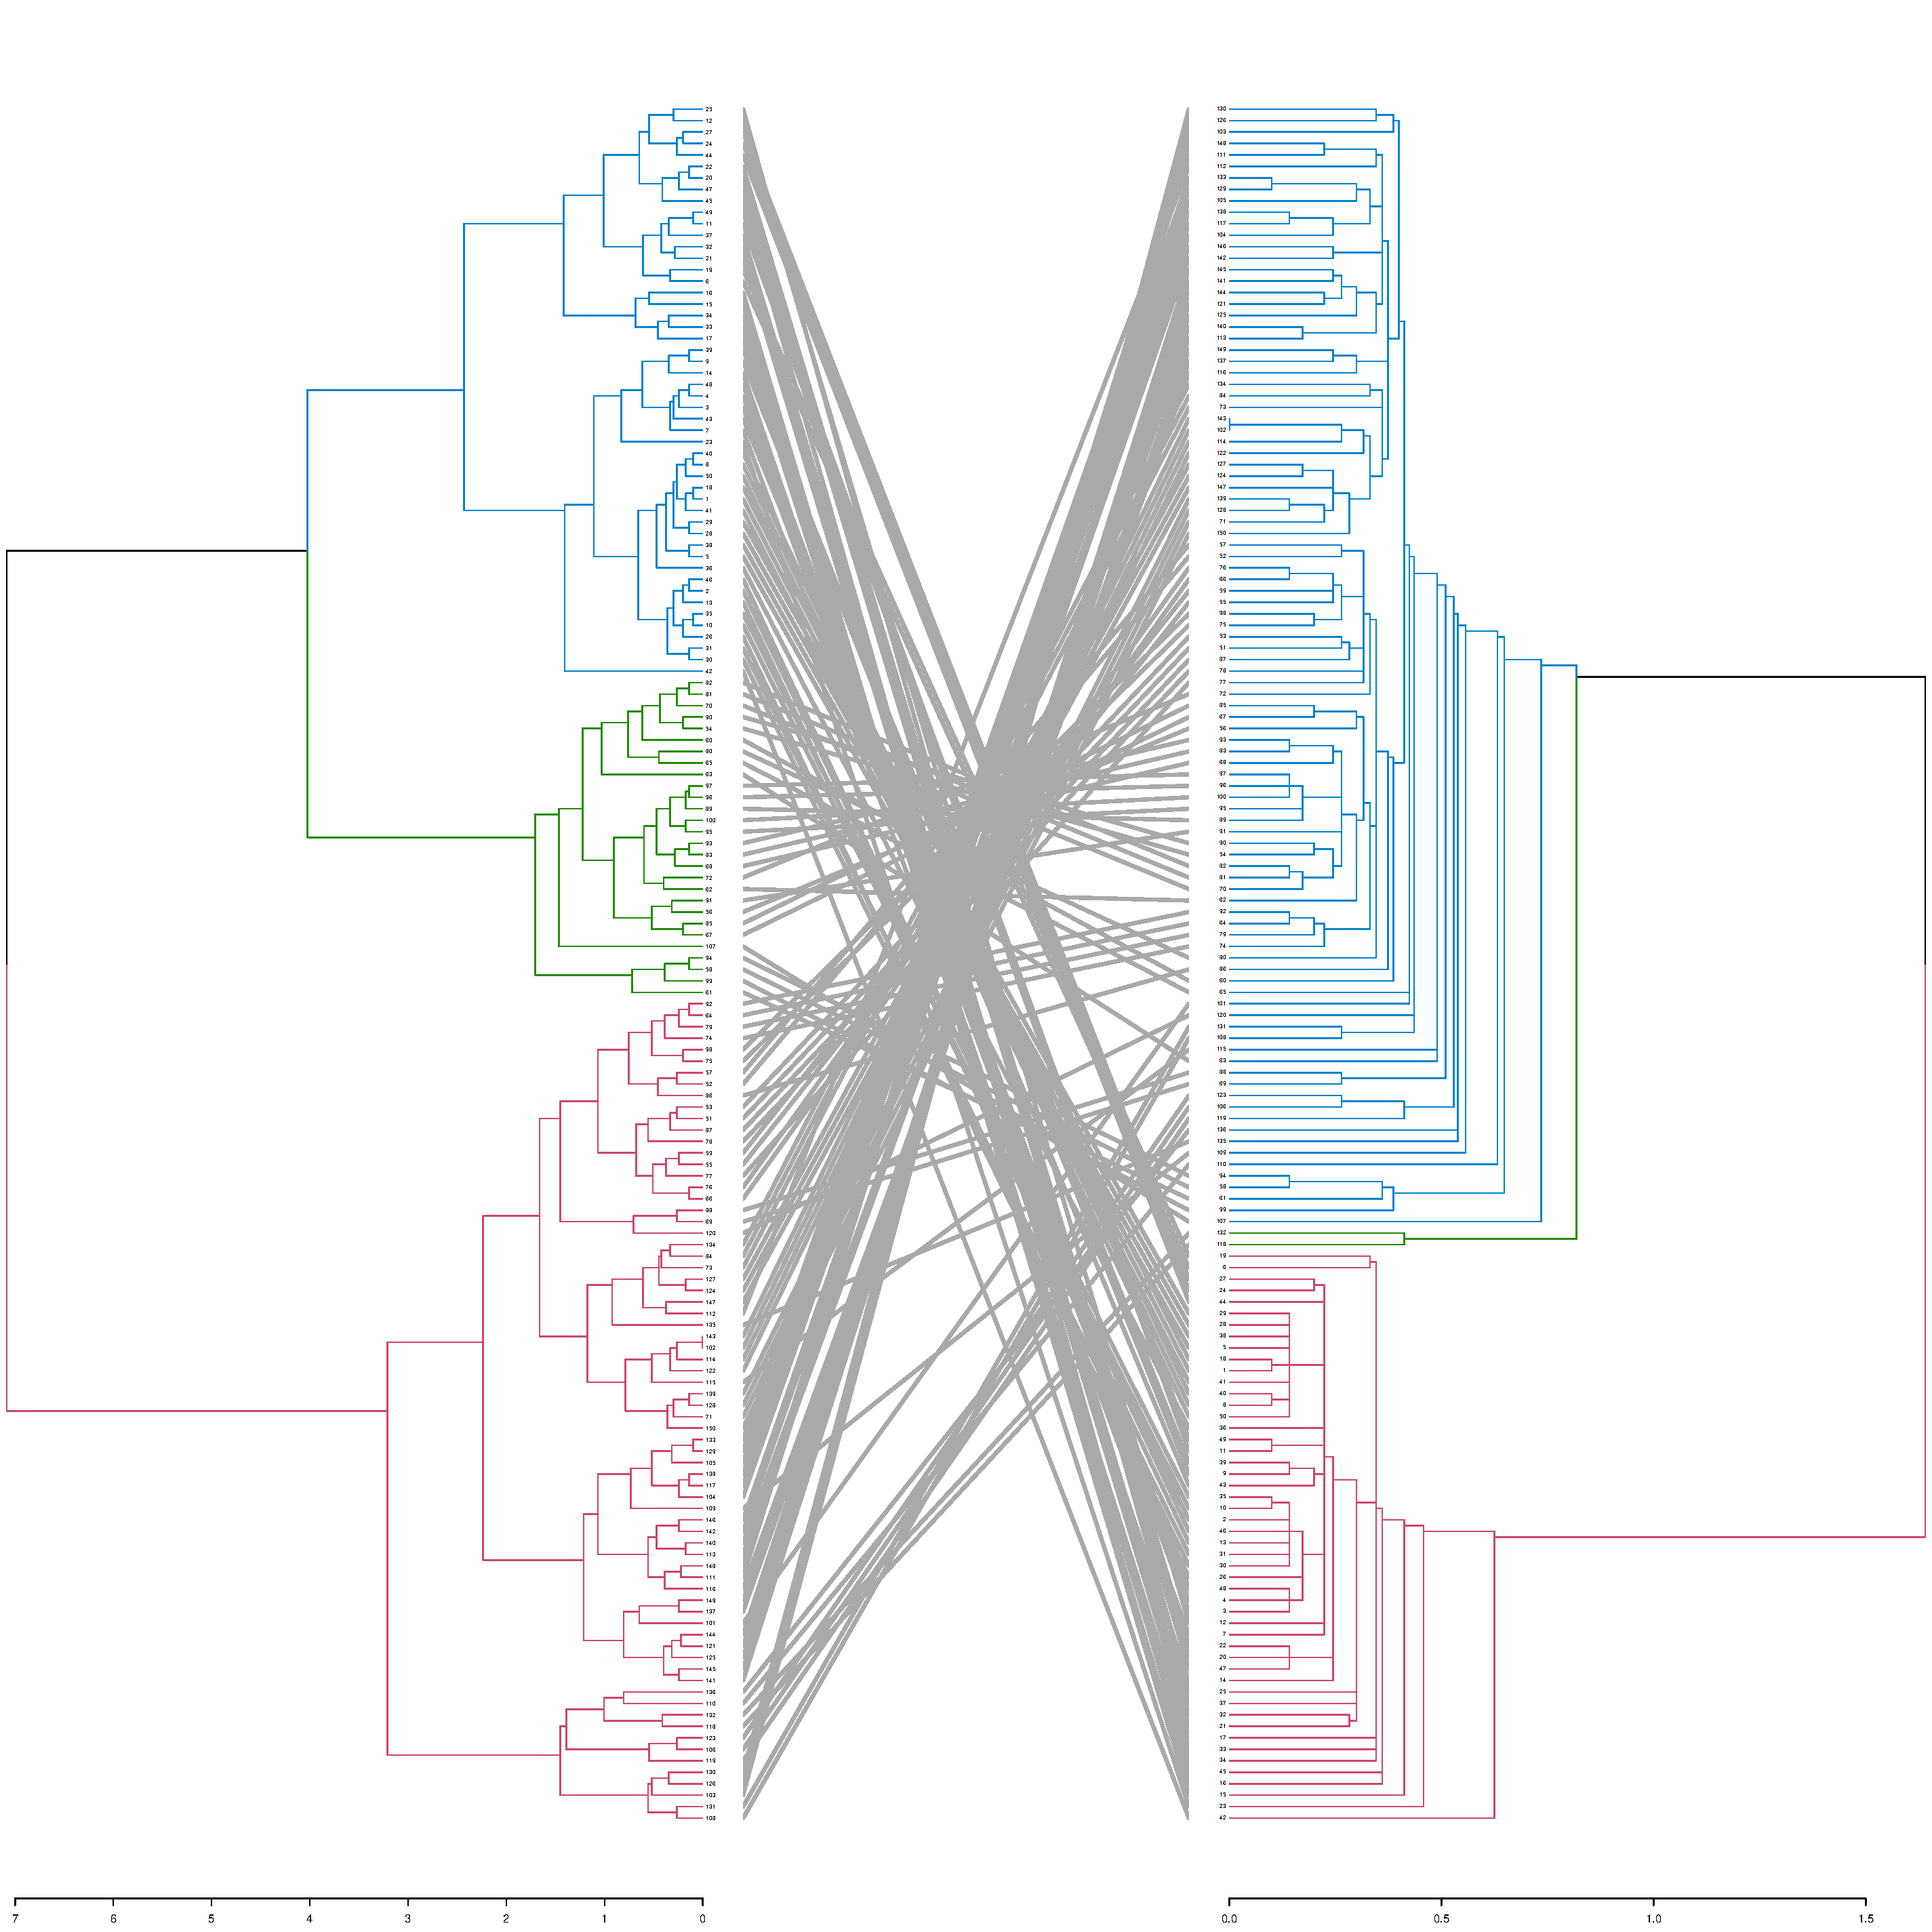
\includegraphics[width=\maxwidth]{figure/first_tanglegram} 

}



\end{knitrout}




Notice that since every manipulation of the trees require going through all of their nodes, it might be better (when comparing large trees), to do all of the manipulations upfront, and only then plot the tanglegram.

We can also notice the mess of tangled lines of the two trees, a mess we wish to untangle.

\subsection{Measuring Entanglement}

When comparing two trees via a tanglegram, we can use the \code{entanglement} function in order to measure how much the two trees are "aligned".

Entanglement is measured by giving the left tree's labels the values of 1 till tree size, and than match these numbers with the right tree. Now, entanglement is the L norm distance between these two vectors.
That is, we take the sum of the absolute difference (each one in the power of L). e.g: \code{sum(abs(x-y)**L)}.
And this is devided by the "worst case" entanglement level (e.g: when the right tree is the complete reverse of the left tree).

L tells us which panelty level we are at (L0, L1, L2, partial L's etc).  L>1 means that we give a big panelty for sharp angles.  While L->0 means that any time something is not a streight horizontal line, it gets a large penalty If L=0.1 it means that we much prefer streight lines over non streight lines


For example:

\begin{knitrout}
\definecolor{shadecolor}{rgb}{0.969, 0.969, 0.969}\color{fgcolor}\begin{kframe}
\begin{alltt}
\hlstd{hc1} \hlkwb{<-} \hlkwd{hclust}\hlstd{(}\hlkwd{dist}\hlstd{(iris[,} \hlopt{-}\hlnum{5}\hlstd{]),} \hlstr{"com"}\hlstd{)}
\hlstd{hc2} \hlkwb{<-} \hlkwd{hclust}\hlstd{(}\hlkwd{dist}\hlstd{(iris[,} \hlopt{-}\hlnum{5}\hlstd{]),} \hlstr{"single"}\hlstd{)}
\hlstd{dend1} \hlkwb{<-} \hlkwd{as.dendrogram}\hlstd{(hc1)}
\hlstd{dend2} \hlkwb{<-} \hlkwd{as.dendrogram}\hlstd{(hc2)}
\hlstd{dend1} \hlkwb{<-} \hlkwd{color_branches}\hlstd{(dend1,} \hlnum{3}\hlstd{)}
\hlcom{# dend2 <- color_branches(dend2, 3) # colors will not match}
\hlcom{# nicely}
\hlkwd{labels}\hlstd{(dend2)} \hlkwb{<-} \hlkwd{as.character}\hlstd{(}\hlkwd{labels}\hlstd{(dend2)}\hlstd{)}

\hlkwd{require}\hlstd{(colorspace}\hlstd{)}

\hlstd{col_lines_by_left_groups} \hlkwb{<-} \hlkwd{rainbow_hcl}\hlstd{(}\hlnum{3}\hlstd{)[}\hlkwd{cutree}\hlstd{(dend1,} \hlnum{3}\hlstd{,} \hlkwc{order_clusters_as_data} \hlstd{=} \hlnum{FALSE}\hlstd{,}
    \hlkwc{sort_cluster_numbers} \hlstd{=} \hlnum{TRUE}\hlstd{)]}
\hlkwd{tanglegram}\hlstd{(dend1, dend2,} \hlkwc{color_lines} \hlstd{= col_lines_by_left_groups,}
    \hlkwc{main} \hlstd{=} \hlkwd{paste}\hlstd{(}\hlstr{"Entanglement ="}\hlstd{,} \hlkwd{round}\hlstd{(}\hlkwd{entanglement}\hlstd{(dend1,}
        \hlstd{dend2),} \hlnum{2}\hlstd{)))}
\end{alltt}
\end{kframe}

{\centering 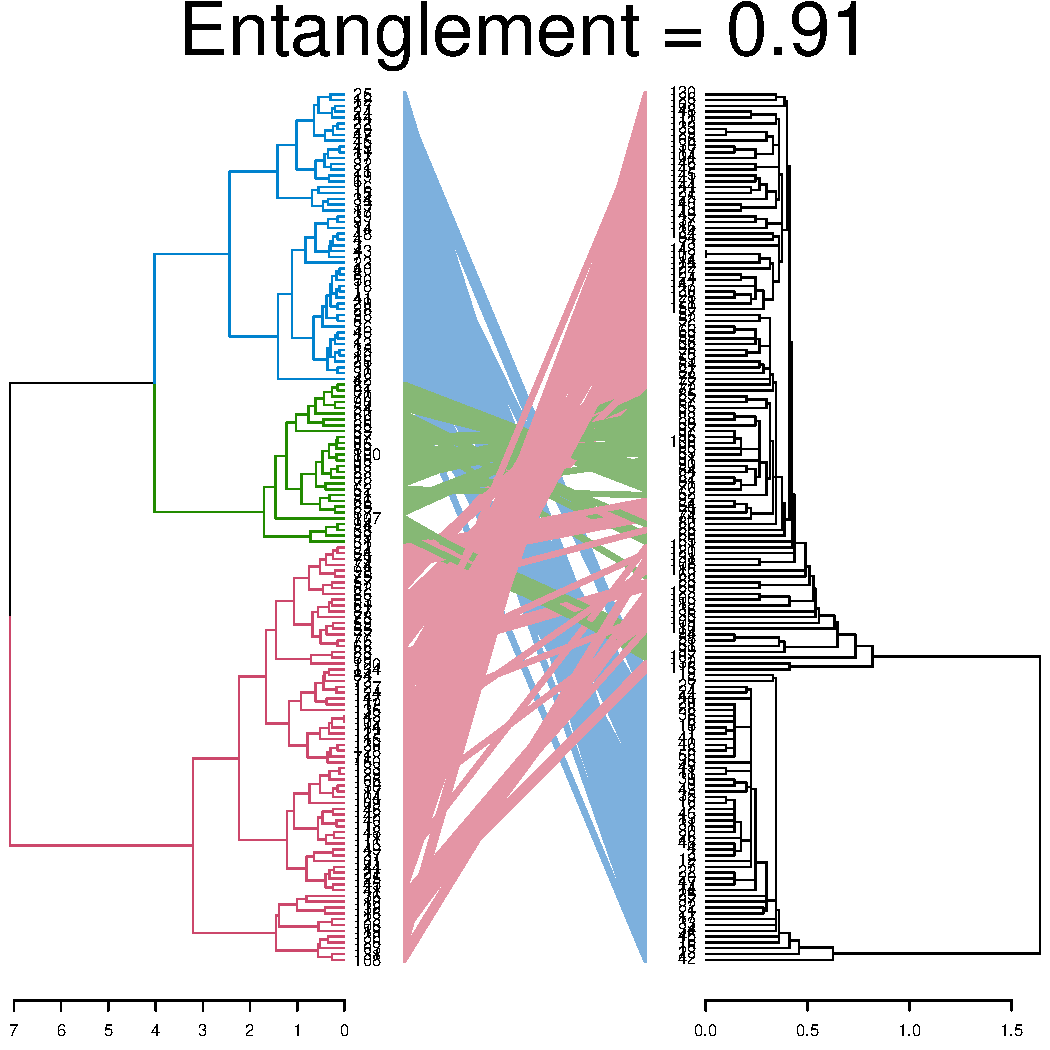
\includegraphics[width=\maxwidth]{figure/unnamed-chunk-32} 

}



\end{knitrout}


And here is the entanglement of a tiny bit prettier tanglegram:

\begin{knitrout}
\definecolor{shadecolor}{rgb}{0.969, 0.969, 0.969}\color{fgcolor}\begin{kframe}
\begin{alltt}
\hlstd{s_dend1} \hlkwb{<-} \hlkwd{sort}\hlstd{(dend1)}
\hlstd{s_dend2} \hlkwb{<-} \hlkwd{sort}\hlstd{(dend2}\hlstd{)}

\hlcom{# s_dend1 <- color_branches(s_dend1, 3) # If I don't do this}
\hlcom{# again I will get different colors}
\hlstd{col_lines_by_left_groups_sorted} \hlkwb{<-} \hlstd{col_lines_by_left_groups[}\hlkwd{match}\hlstd{(}\hlkwd{labels}\hlstd{(s_dend1),}
    \hlkwd{labels}\hlstd{(dend1))]}
\hlkwd{tanglegram}\hlstd{(s_dend1, s_dend2,} \hlkwc{color_lines} \hlstd{= col_lines_by_left_groups_sorted,}
    \hlkwc{main} \hlstd{=} \hlkwd{paste}\hlstd{(}\hlstr{"Entanglement ="}\hlstd{,} \hlkwd{round}\hlstd{(}\hlkwd{entanglement}\hlstd{(s_dend1,}
        \hlstd{s_dend2),} \hlnum{2}\hlstd{)))}
\end{alltt}
\end{kframe}

{\centering 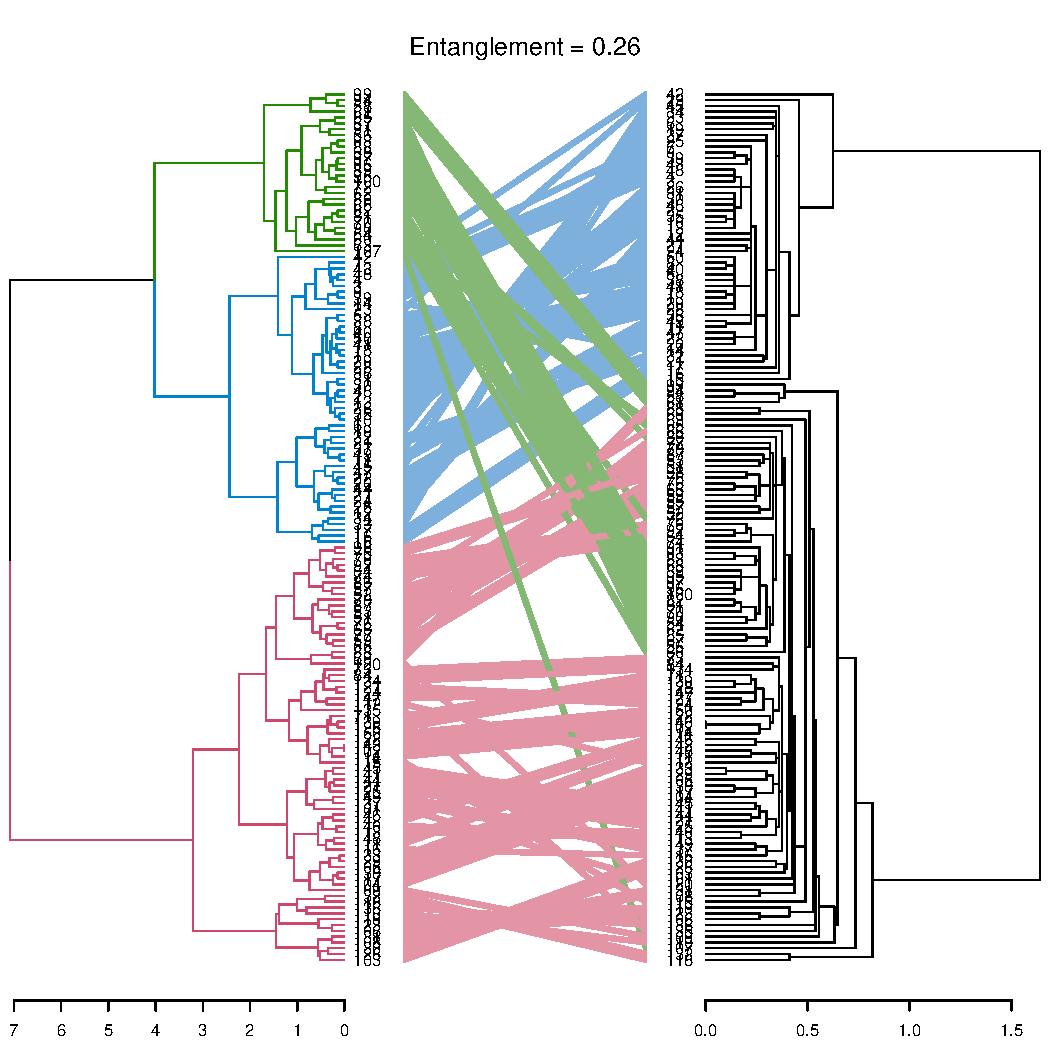
\includegraphics[width=\maxwidth]{figure/unnamed-chunk-33} 

}



\end{knitrout}




\subsection{Finding an optimal rotation}

\subsubsection{Random search}


Finding an optimal rotation for the tanglegram of two dendrogram is a hard problem.
%% ref here.

This problem is also harder for larger trees, so let us pick a tree from only 30 flowers, and look at comparing two clustering methods, complete and single:


\begin{knitrout}
\definecolor{shadecolor}{rgb}{0.969, 0.969, 0.969}\color{fgcolor}\begin{kframe}
\begin{alltt}
\hlkwd{set.seed}\hlstd{(}\hlnum{51324626}\hlstd{)}
\hlstd{ss} \hlkwb{<-} \hlkwd{sample}\hlstd{(}\hlnum{1}\hlopt{:}\hlnum{150}\hlstd{,} \hlkwc{size} \hlstd{=} \hlnum{30}\hlstd{)}
\hlstd{hc1} \hlkwb{<-} \hlkwd{hclust}\hlstd{(}\hlkwd{dist}\hlstd{(iris[ss,} \hlopt{-}\hlnum{5}\hlstd{]),} \hlstr{"com"}\hlstd{)}
\hlstd{hc2} \hlkwb{<-} \hlkwd{hclust}\hlstd{(}\hlkwd{dist}\hlstd{(iris[ss,} \hlopt{-}\hlnum{5}\hlstd{]),} \hlstr{"single"}\hlstd{)}
\hlstd{dend1} \hlkwb{<-} \hlkwd{as.dendrogram}\hlstd{(hc1)}
\hlstd{dend2} \hlkwb{<-} \hlkwd{as.dendrogram}\hlstd{(hc2)}
\hlstd{dend1} \hlkwb{<-} \hlkwd{color_branches}\hlstd{(dend1,} \hlnum{3}\hlstd{)}
\hlcom{# dend2 <- color_branches(dend2, 3) # colors will not match}
\hlcom{# nicely}
\hlkwd{labels}\hlstd{(dend2)} \hlkwb{<-} \hlkwd{as.character}\hlstd{(}\hlkwd{labels}\hlstd{(dend2)}\hlstd{)}

\hlkwd{require}\hlstd{(colorspace}\hlstd{)}

\hlstd{col_lines_by_left_groups} \hlkwb{<-} \hlkwd{rainbow_hcl}\hlstd{(}\hlnum{3}\hlstd{)[}\hlkwd{cutree}\hlstd{(dend1,} \hlnum{3}\hlstd{,} \hlkwc{order_clusters_as_data} \hlstd{=} \hlnum{FALSE}\hlstd{,}
    \hlkwc{sort_cluster_numbers} \hlstd{=} \hlnum{TRUE}\hlstd{)]}
\hlkwd{tanglegram}\hlstd{(dend1, dend2,} \hlkwc{color_lines} \hlstd{= col_lines_by_left_groups,}
    \hlkwc{main} \hlstd{=} \hlkwd{paste}\hlstd{(}\hlstr{"Entanglement ="}\hlstd{,} \hlkwd{round}\hlstd{(}\hlkwd{entanglement}\hlstd{(dend1,}
        \hlstd{dend2),} \hlnum{2}\hlstd{)))}
\end{alltt}
\end{kframe}

{\centering 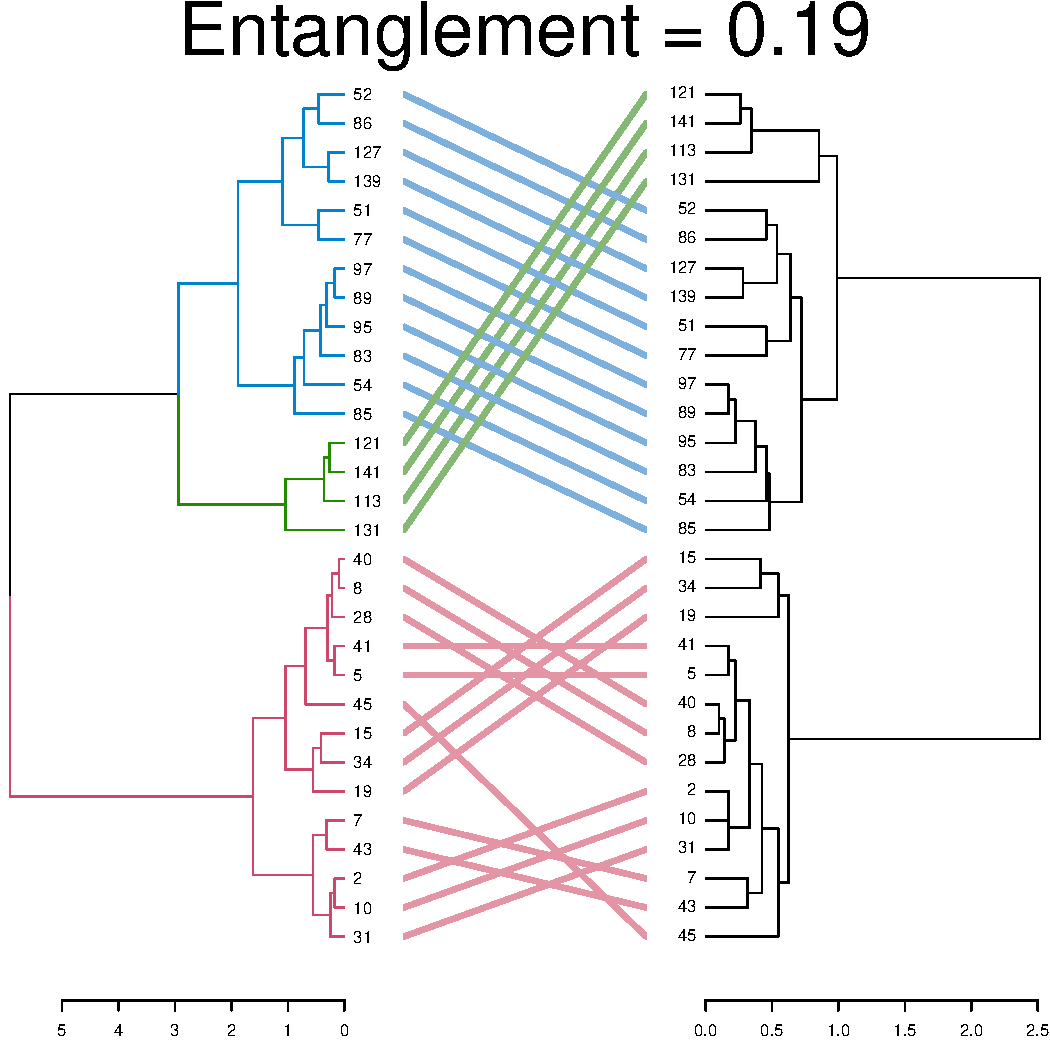
\includegraphics[width=\maxwidth]{figure/unnamed-chunk-34} 

}



\end{knitrout}


One solution for improving the tanglegram would be to randomely search the rotated tree space for a better solution.

For example:

\begin{knitrout}
\definecolor{shadecolor}{rgb}{0.969, 0.969, 0.969}\color{fgcolor}\begin{kframe}
\begin{alltt}
\hlkwd{set.seed}\hlstd{(}\hlnum{65168}\hlstd{)}
\hlstd{dend12} \hlkwb{<-} \hlkwd{untangle_random_search}\hlstd{(dend1, dend2,} \hlkwc{R} \hlstd{=} \hlnum{100}\hlstd{)}
\hlkwd{tanglegram}\hlstd{(dend12[[}\hlnum{1}\hlstd{]], dend12[[}\hlnum{2}\hlstd{]],} \hlkwc{color_lines} \hlstd{= col_lines_by_left_groups,}
    \hlkwc{main} \hlstd{=} \hlkwd{paste}\hlstd{(}\hlstr{"Entanglement ="}\hlstd{,} \hlkwd{round}\hlstd{(}\hlkwd{entanglement}\hlstd{(dend12[[}\hlnum{1}\hlstd{]],}
        \hlstd{dend12[[}\hlnum{2}\hlstd{]]),} \hlnum{2}\hlstd{)))}
\end{alltt}
\end{kframe}

{\centering 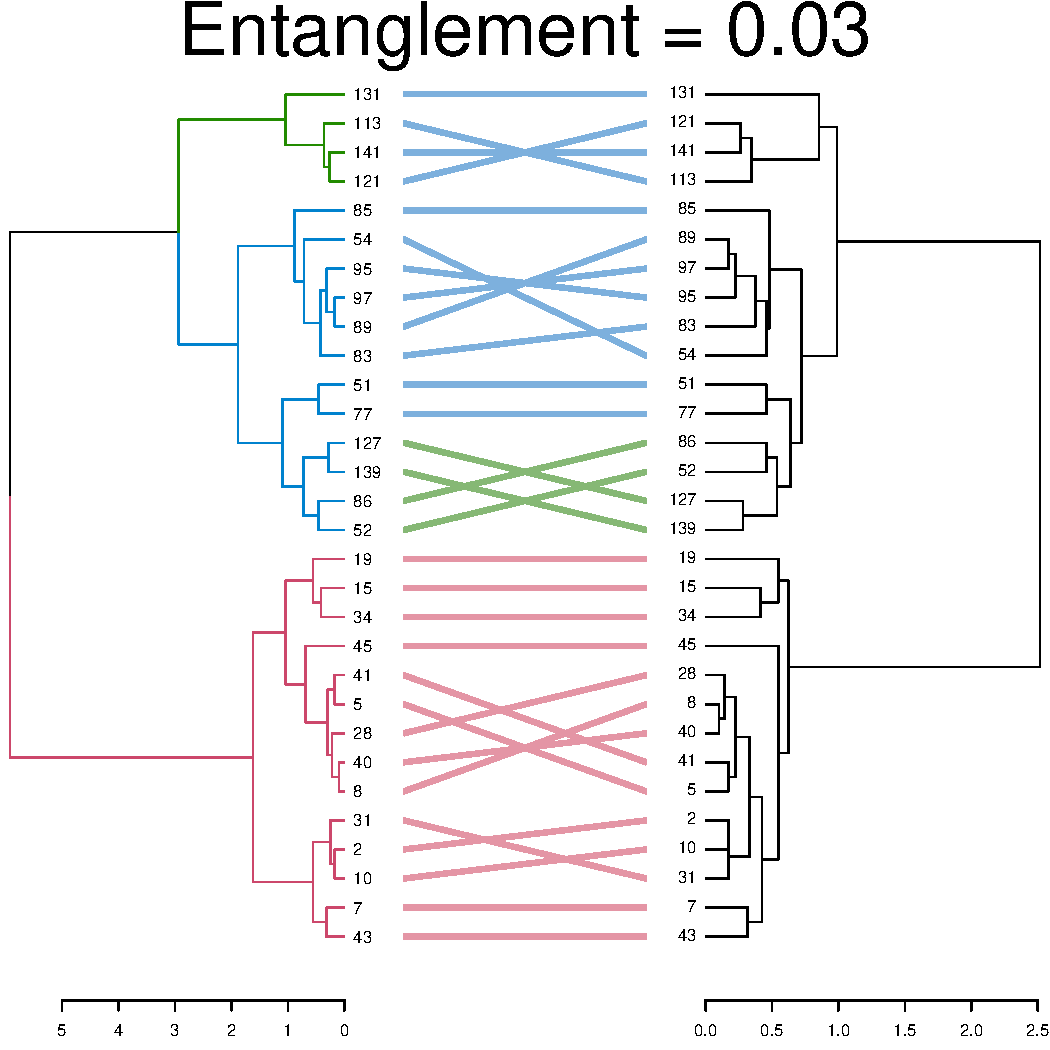
\includegraphics[width=\maxwidth]{figure/unnamed-chunk-35} 

}



\end{knitrout}


We can see we already got something better. An advantage of the random search is the ability to create many many trees and compare them to find the best pair.


\subsubsection{A one-side greedy search}

Let's use a greedy forward step wise rotation of the right tree, to see if we can find a better solution for comparing the two trees. Notice that this may take some time to run (the larger the tree, the longer it would take), but we can limit the search for smaller k's, and see what improvement that can bring us:


\begin{knitrout}
\definecolor{shadecolor}{rgb}{0.969, 0.969, 0.969}\color{fgcolor}\begin{kframe}
\begin{alltt}
\hlstd{best_dend_heights_per_k} \hlkwb{<-} \hlkwd{heights_per_k.dendrogram}\hlstd{(dend2}\hlstd{)}

\hlstd{dend2_2} \hlkwb{<-} \hlkwd{untangle_step_rotate_1side}\hlstd{(dend2, dend1,} \hlkwc{k_seq} \hlstd{=} \hlnum{2}\hlopt{:}\hlnum{3}\hlstd{,}
    \hlkwc{best_dend_heights_per_k} \hlstd{= best_dend_heights_per_k)}
\end{alltt}


{\ttfamily\noindent\itshape\color{messagecolor}{\#\# Loading required package: plyr}}\begin{alltt}
\hlcom{# notice that here we are only using}
\hlkwd{tanglegram}\hlstd{(dend1, dend2_2,} \hlkwc{color_lines} \hlstd{= col_lines_by_left_groups,}
    \hlkwc{main} \hlstd{=} \hlkwd{paste}\hlstd{(}\hlstr{"Entanglement ="}\hlstd{,} \hlkwd{round}\hlstd{(}\hlkwd{entanglement}\hlstd{(dend1,}
        \hlstd{dend2_2),} \hlnum{2}\hlstd{)))}
\end{alltt}
\end{kframe}

{\centering 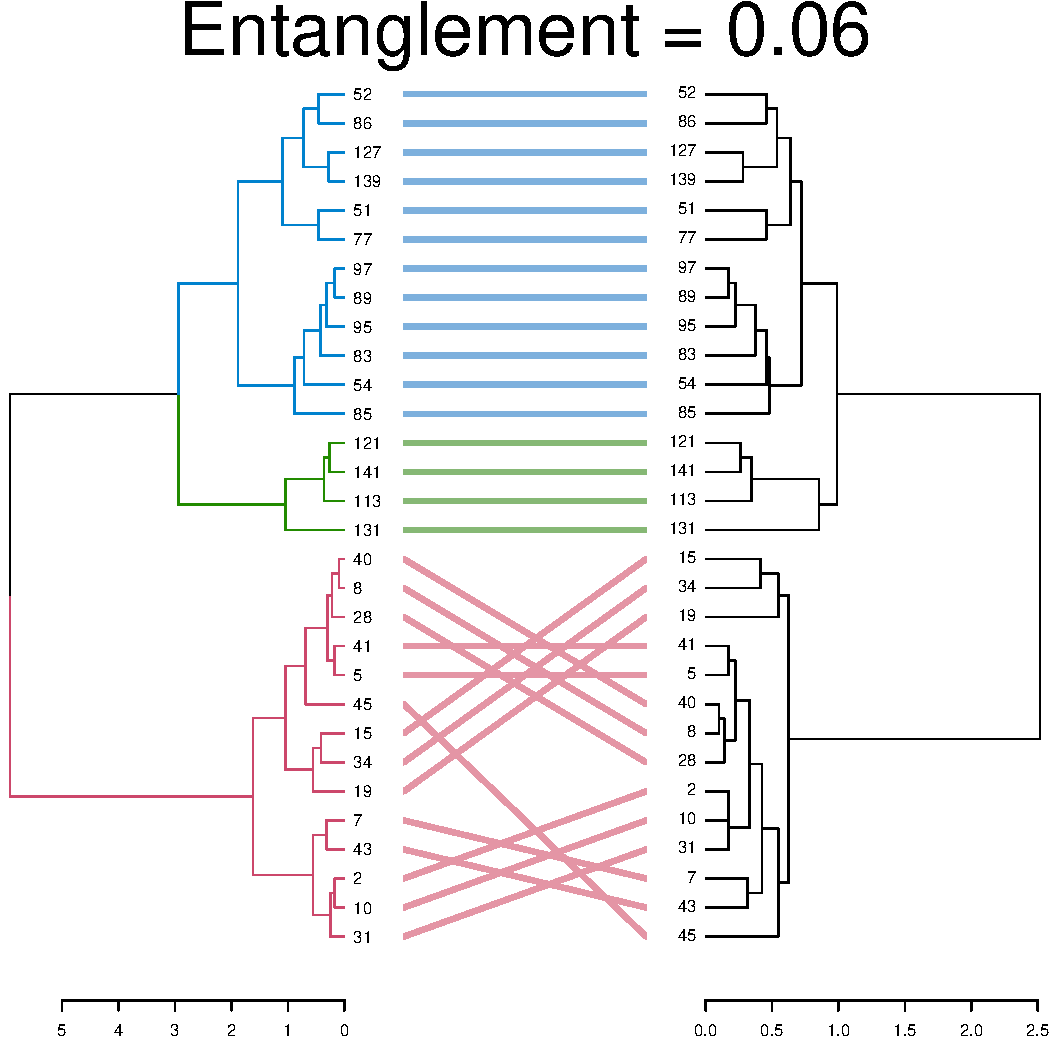
\includegraphics[width=\maxwidth]{figure/unnamed-chunk-36} 

}


\begin{kframe}\begin{alltt}
\hlkwd{entanglement}\hlstd{(dend1, dend2_2)}
\end{alltt}
\begin{verbatim}
## [1] 0.06166
\end{verbatim}
\end{kframe}
\end{knitrout}



Let's try to go "all the way down" all possible k's:

\begin{knitrout}
\definecolor{shadecolor}{rgb}{0.969, 0.969, 0.969}\color{fgcolor}\begin{kframe}
\begin{alltt}
\hlstd{dend2_3} \hlkwb{<-} \hlkwd{untangle_step_rotate_1side}\hlstd{(dend2, dend1,} \hlkwc{best_dend_heights_per_k} \hlstd{= best_dend_heights_per_k)}
\hlkwd{tanglegram}\hlstd{(dend1, dend2_3,} \hlkwc{color_lines} \hlstd{= col_lines_by_left_groups,}
    \hlkwc{main} \hlstd{=} \hlkwd{paste}\hlstd{(}\hlstr{"Entanglement ="}\hlstd{,} \hlkwd{round}\hlstd{(}\hlkwd{entanglement}\hlstd{(dend1,}
        \hlstd{dend2_3),} \hlnum{2}\hlstd{)))}
\end{alltt}
\end{kframe}

{\centering 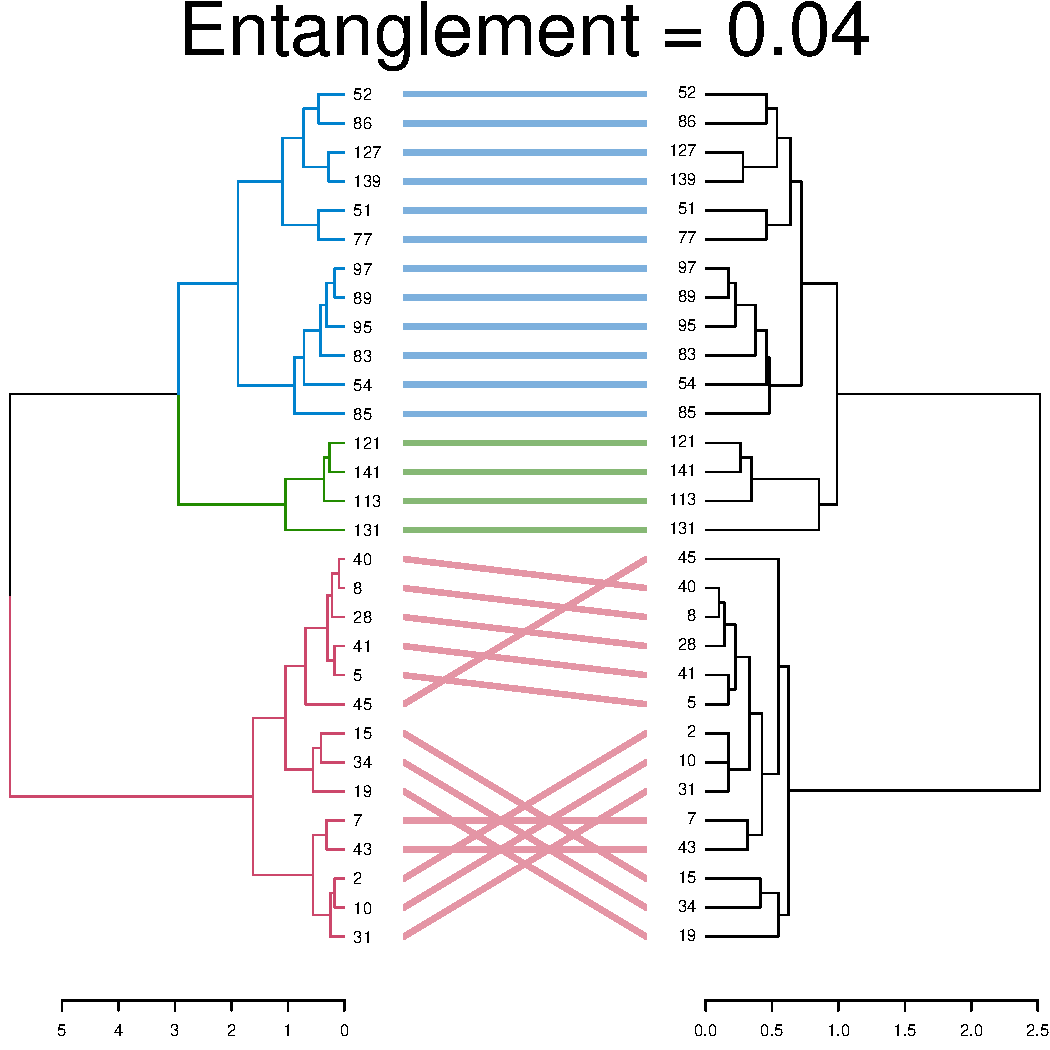
\includegraphics[width=\maxwidth]{figure/unnamed-chunk-37} 

}


\begin{kframe}\begin{alltt}
\hlkwd{entanglement}\hlstd{(dend1, dend2_3)}
\end{alltt}
\begin{verbatim}
## [1] 0.04225
\end{verbatim}
\begin{alltt}

\end{alltt}
\end{kframe}
\end{knitrout}


\subsubsection{Combining a one-side greedy search with a random search}

As we can see, the random search actually found something better than the forward selection search. But now we can use the forward search on the trees we found in the random search:


\begin{knitrout}
\definecolor{shadecolor}{rgb}{0.969, 0.969, 0.969}\color{fgcolor}\begin{kframe}
\begin{alltt}
\hlstd{dend2_4} \hlkwb{<-} \hlkwd{untangle_step_rotate_1side}\hlstd{(dend12[[}\hlnum{2}\hlstd{]], dend12[[}\hlnum{1}\hlstd{]])}
\hlkwd{tanglegram}\hlstd{(dend12[[}\hlnum{1}\hlstd{]], dend2_4,} \hlkwc{color_lines} \hlstd{= col_lines_by_left_groups,}
    \hlkwc{main} \hlstd{=} \hlkwd{paste}\hlstd{(}\hlstr{"Entanglement ="}\hlstd{,} \hlkwd{round}\hlstd{(}\hlkwd{entanglement}\hlstd{(dend12[[}\hlnum{1}\hlstd{]],}
        \hlstd{dend2_4),} \hlnum{2}\hlstd{)))}
\end{alltt}
\end{kframe}

{\centering 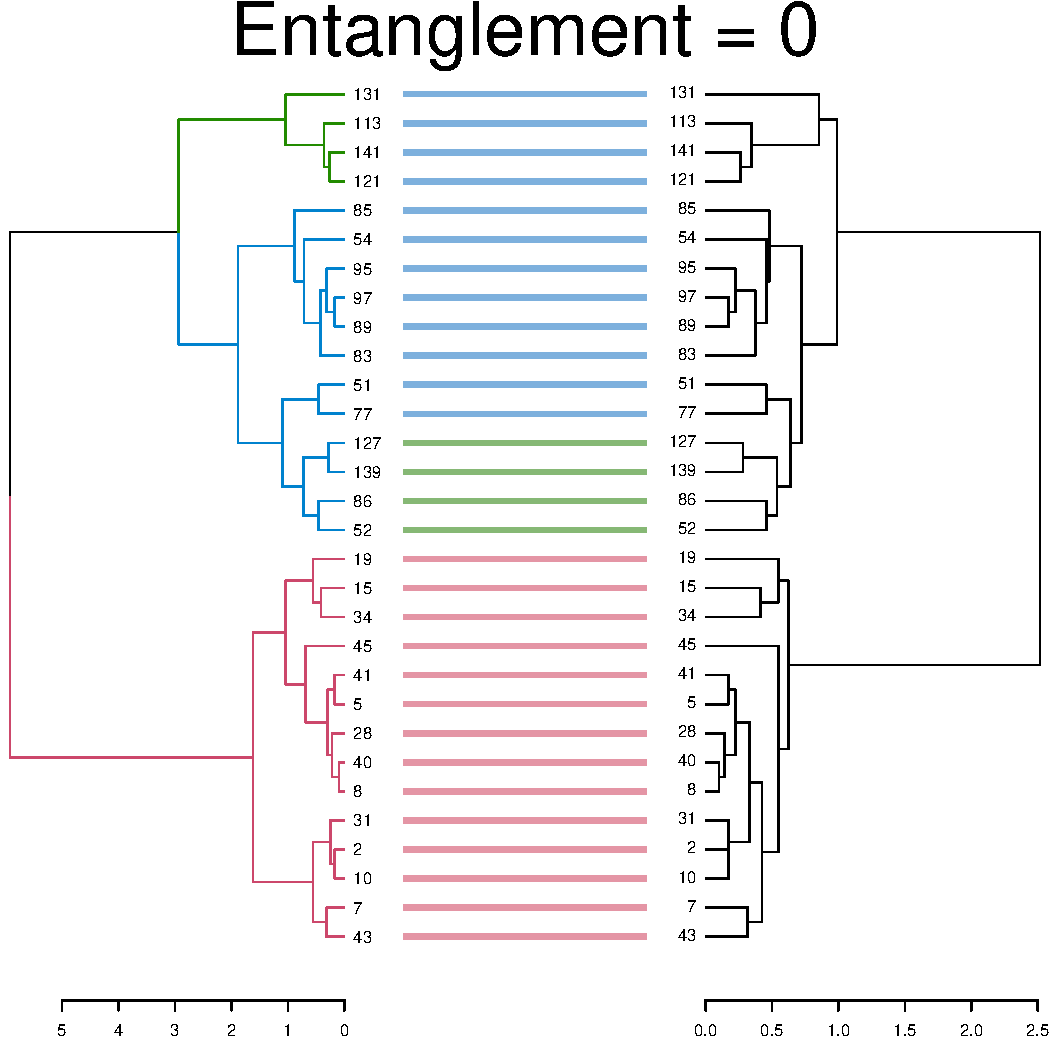
\includegraphics[width=\maxwidth]{figure/unnamed-chunk-38} 

}


\begin{kframe}\begin{alltt}
\hlkwd{entanglement}\hlstd{(dend12[[}\hlnum{1}\hlstd{]], dend2_4)}
\end{alltt}
\begin{verbatim}
## [1] 0
\end{verbatim}
\begin{alltt}

\end{alltt}
\end{kframe}
\end{knitrout}


We see how this got us with a perfect solution. The trees look almost identical, but they are not (look at label 45 to see a leaf which is differently located between the two trees.). We can use the \code{k_branches} parameter for tanglegram, to help us see the difference between the two trees (notice labels 19 and 45). One could actually do an animation sequence, using various \code{k_branches} values in order to located the differences between the trees.

\begin{knitrout}
\definecolor{shadecolor}{rgb}{0.969, 0.969, 0.969}\color{fgcolor}\begin{kframe}
\begin{alltt}
\hlkwd{tanglegram}\hlstd{(}\hlkwd{color_branches}\hlstd{(dend12[[}\hlnum{1}\hlstd{]],} \hlkwc{col} \hlstd{=} \hlnum{1}\hlstd{,} \hlkwc{k} \hlstd{=} \hlnum{1}\hlstd{), dend2_4,}
    \hlkwc{color_lines} \hlstd{= col_lines_by_left_groups,} \hlkwc{k_branches} \hlstd{=} \hlnum{10}\hlstd{,}
    \hlkwc{main} \hlstd{=} \hlkwd{paste}\hlstd{(}\hlstr{"Entanglement ="}\hlstd{,} \hlkwd{round}\hlstd{(}\hlkwd{entanglement}\hlstd{(dend12[[}\hlnum{1}\hlstd{]],}
        \hlstd{dend2_4),} \hlnum{2}\hlstd{)))}
\end{alltt}
\end{kframe}

{\centering 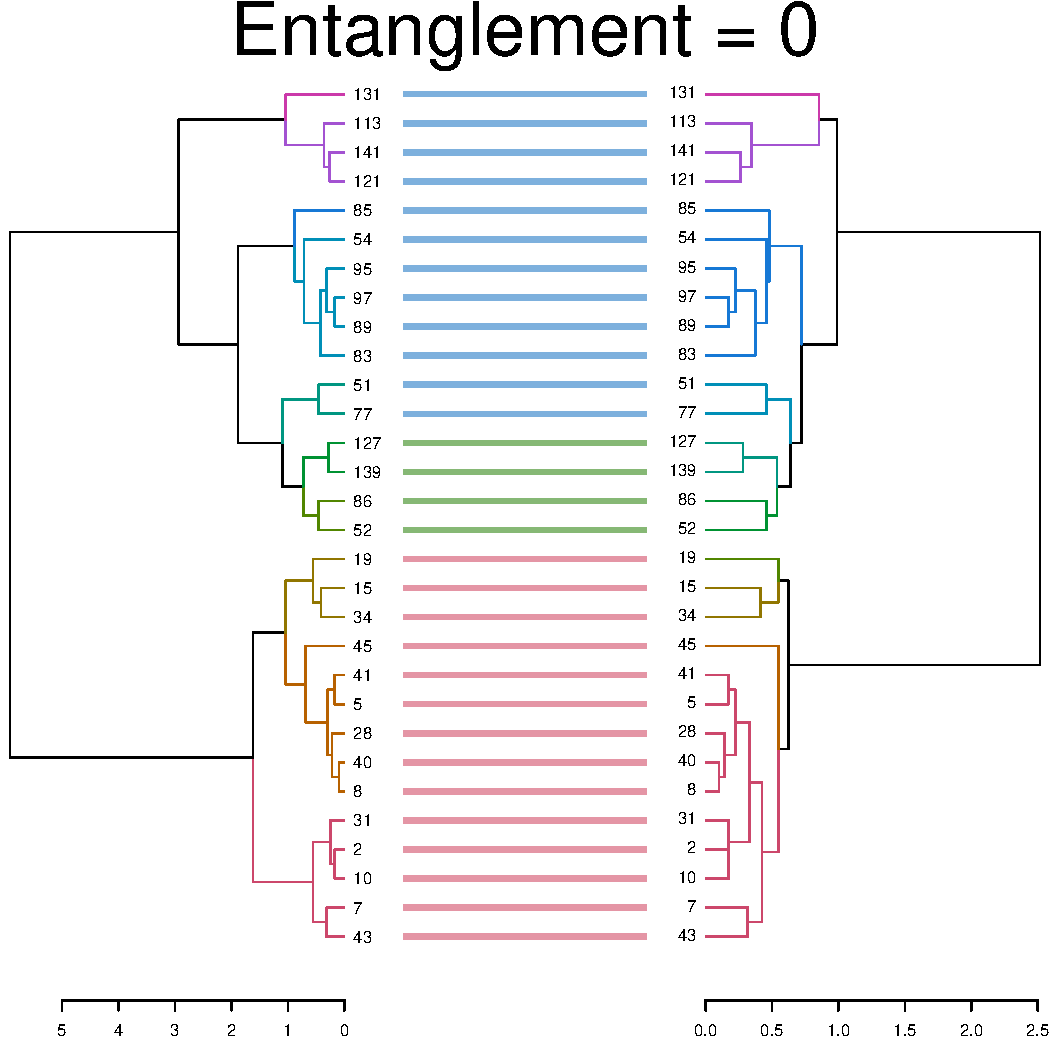
\includegraphics[width=\maxwidth]{figure/unnamed-chunk-39} 

}



\end{knitrout}



\subsubsection{A two-side greedy search}

Sometimes, using just one-sise greedy algorithm is not enough. Also, it is probably best to combine the random search with the two sided greedy stepwise search:

\begin{knitrout}
\definecolor{shadecolor}{rgb}{0.969, 0.969, 0.969}\color{fgcolor}\begin{kframe}
\begin{alltt}
\hlstd{dend1} \hlkwb{<-} \hlkwd{as.dendrogram}\hlstd{(}\hlkwd{hclust}\hlstd{(}\hlkwd{dist}\hlstd{(USArrests[}\hlnum{1}\hlopt{:}\hlnum{20}\hlstd{, ])))}
\hlstd{dend2} \hlkwb{<-} \hlkwd{as.dendrogram}\hlstd{(}\hlkwd{hclust}\hlstd{(}\hlkwd{dist}\hlstd{(USArrests[}\hlnum{1}\hlopt{:}\hlnum{20}\hlstd{, ]),} \hlkwc{method} \hlstd{=} \hlstr{"single"}\hlstd{))}
\hlkwd{set.seed}\hlstd{(}\hlnum{3525}\hlstd{)}
\hlstd{dend2} \hlkwb{<-} \hlkwd{shuffle}\hlstd{(dend2)}
\hlkwd{tanglegram}\hlstd{(dend1, dend2,} \hlkwc{margin_inner} \hlstd{=} \hlnum{6.5}\hlstd{)}
\end{alltt}
\end{kframe}

{\centering 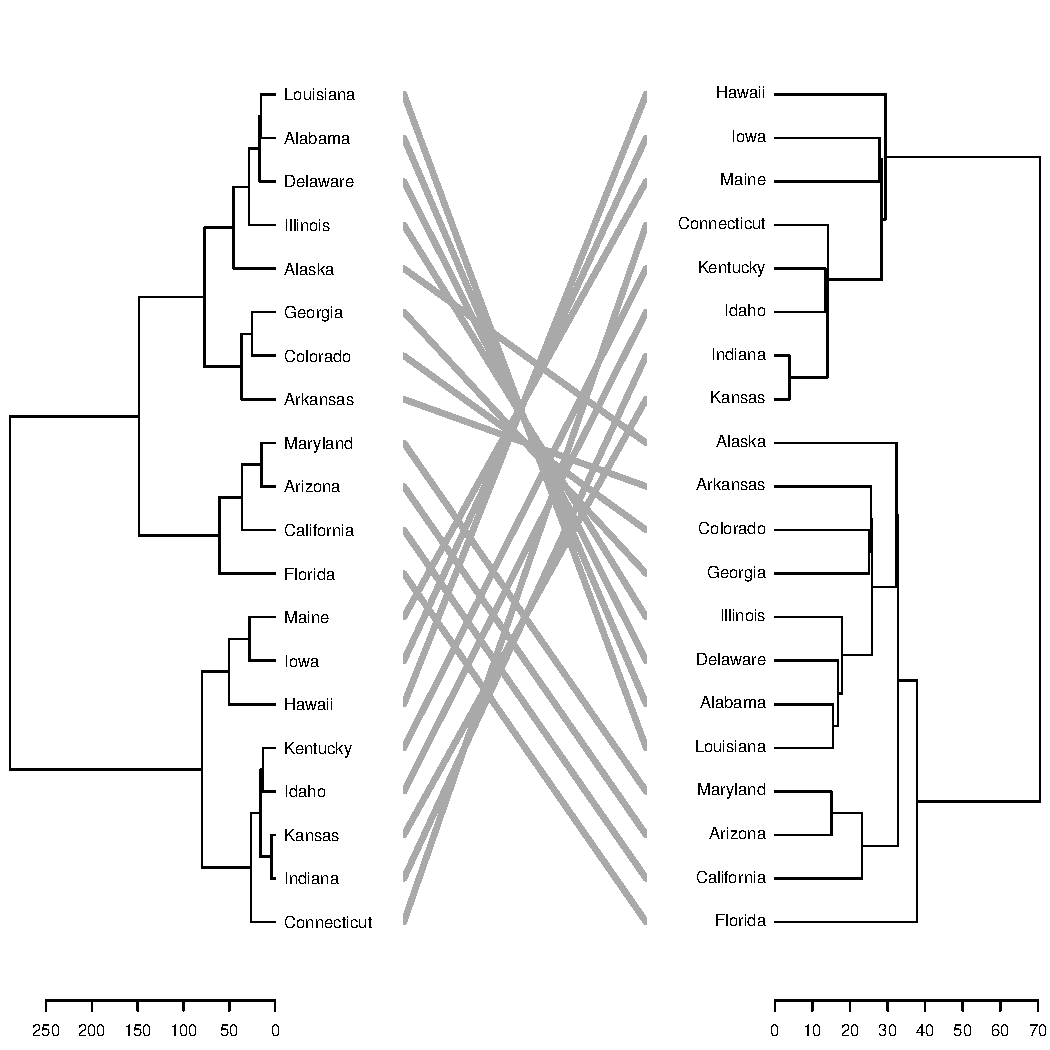
\includegraphics[width=\maxwidth]{figure/untangle_step_rotate_2side_example1} 

}


\begin{kframe}\begin{alltt}
\hlkwd{entanglement}\hlstd{(dend1, dend2,} \hlkwc{L} \hlstd{=} \hlnum{2}\hlstd{)}  \hlcom{# 0.79}
\end{alltt}
\begin{verbatim}
## [1] 0.7917
\end{verbatim}
\begin{alltt}
\hlstd{dend2_corrected} \hlkwb{<-} \hlkwd{untangle_step_rotate_1side}\hlstd{(dend2, dend1)}
\hlkwd{tanglegram}\hlstd{(dend1, dend2_corrected,} \hlkwc{margin_inner} \hlstd{=} \hlnum{6.5}\hlstd{)}  \hlcom{# Good.}
\end{alltt}
\end{kframe}

{\centering 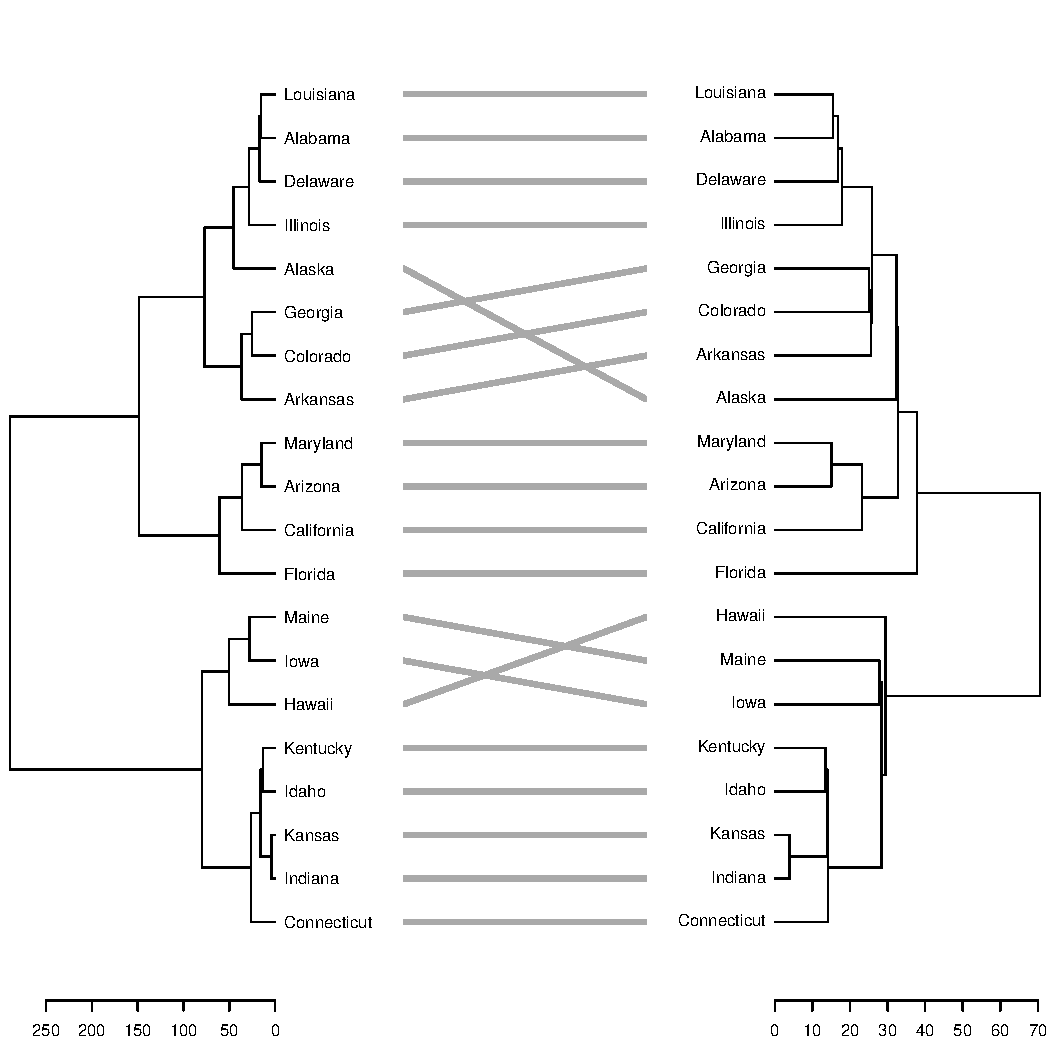
\includegraphics[width=\maxwidth]{figure/untangle_step_rotate_2side_example2} 

}


\begin{kframe}\begin{alltt}
\hlkwd{entanglement}\hlstd{(dend1, dend2_corrected,} \hlkwc{L} \hlstd{=} \hlnum{2}\hlstd{)}  \hlcom{# 0.0067}
\end{alltt}
\begin{verbatim}
## [1] 0.006767
\end{verbatim}
\begin{alltt}
\hlcom{# it is better, but not perfect. Can we improve it?}

\hlstd{dend12_corrected} \hlkwb{<-} \hlkwd{untangle_step_rotate_2side}\hlstd{(dend1, dend2)}
\end{alltt}
\begin{verbatim}
## We ran untangle  1  times
\end{verbatim}
\begin{alltt}
\hlkwd{tanglegram}\hlstd{(dend12_corrected[[}\hlnum{1}\hlstd{]], dend12_corrected[[}\hlnum{2}\hlstd{]],} \hlkwc{margin_inner} \hlstd{=} \hlnum{6.5}\hlstd{)}  \hlcom{# Better...}
\end{alltt}
\end{kframe}

{\centering 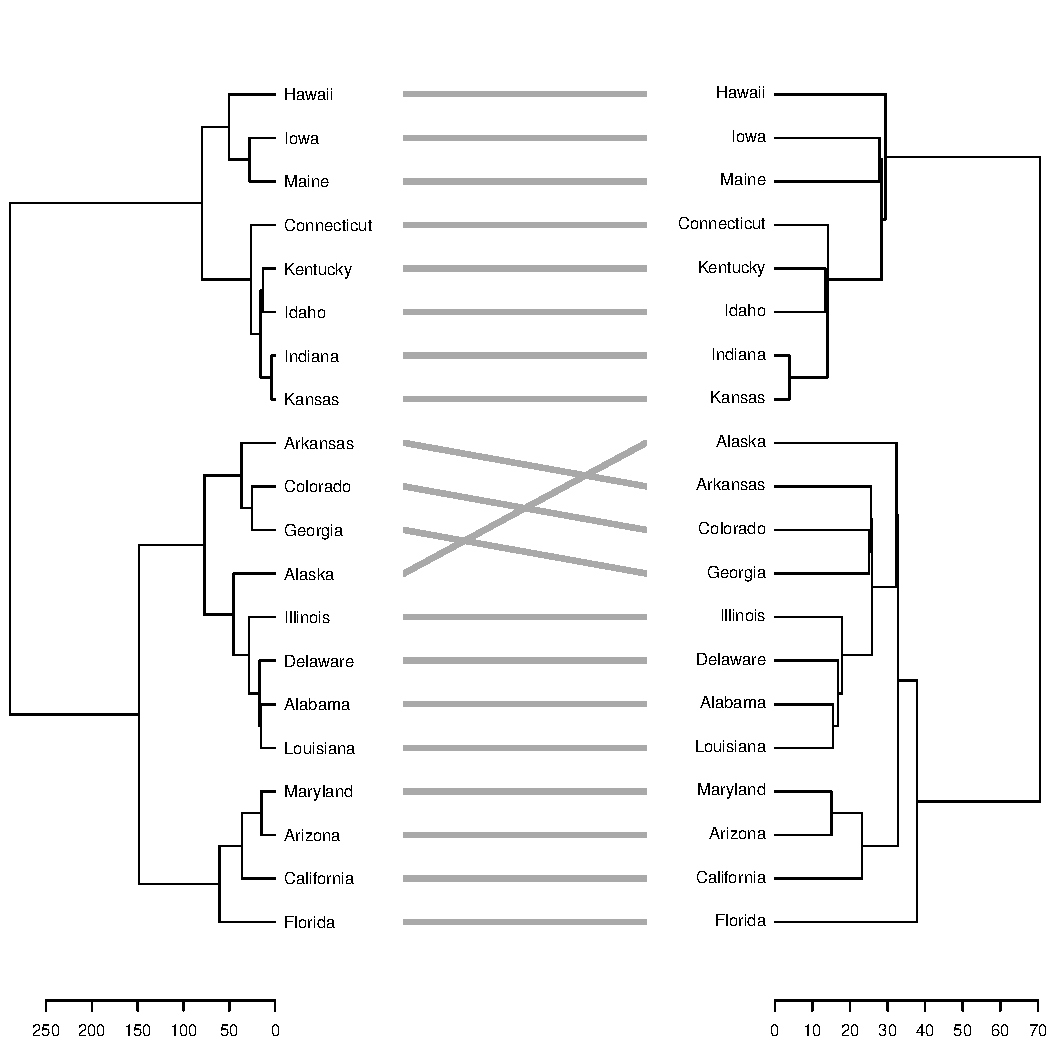
\includegraphics[width=\maxwidth]{figure/untangle_step_rotate_2side_example3} 

}


\begin{kframe}\begin{alltt}
\hlkwd{entanglement}\hlstd{(dend12_corrected[[}\hlnum{1}\hlstd{]], dend12_corrected[[}\hlnum{2}\hlstd{]],} \hlkwc{L} \hlstd{=} \hlnum{2}\hlstd{)}  \hlcom{# 0.0045}
\end{alltt}
\begin{verbatim}
## [1] 0.004511
\end{verbatim}
\begin{alltt}
\hlcom{# best combination:}
\hlstd{dend12_corrected_1} \hlkwb{<-} \hlkwd{untangle_random_search}\hlstd{(dend1, dend2)}
\hlstd{dend12_corrected_2} \hlkwb{<-} \hlkwd{untangle_step_rotate_2side}\hlstd{(dend12_corrected_1[[}\hlnum{1}\hlstd{]],}
    \hlstd{dend12_corrected_1[[}\hlnum{2}\hlstd{]])}
\end{alltt}
\begin{verbatim}
## We ran untangle  1  times
\end{verbatim}
\begin{alltt}
\hlkwd{tanglegram}\hlstd{(dend12_corrected_2[[}\hlnum{1}\hlstd{]], dend12_corrected_2[[}\hlnum{2}\hlstd{]],}
    \hlkwc{margin_inner} \hlstd{=} \hlnum{6.5}\hlstd{)}  \hlcom{# Better...}
\end{alltt}
\end{kframe}

{\centering 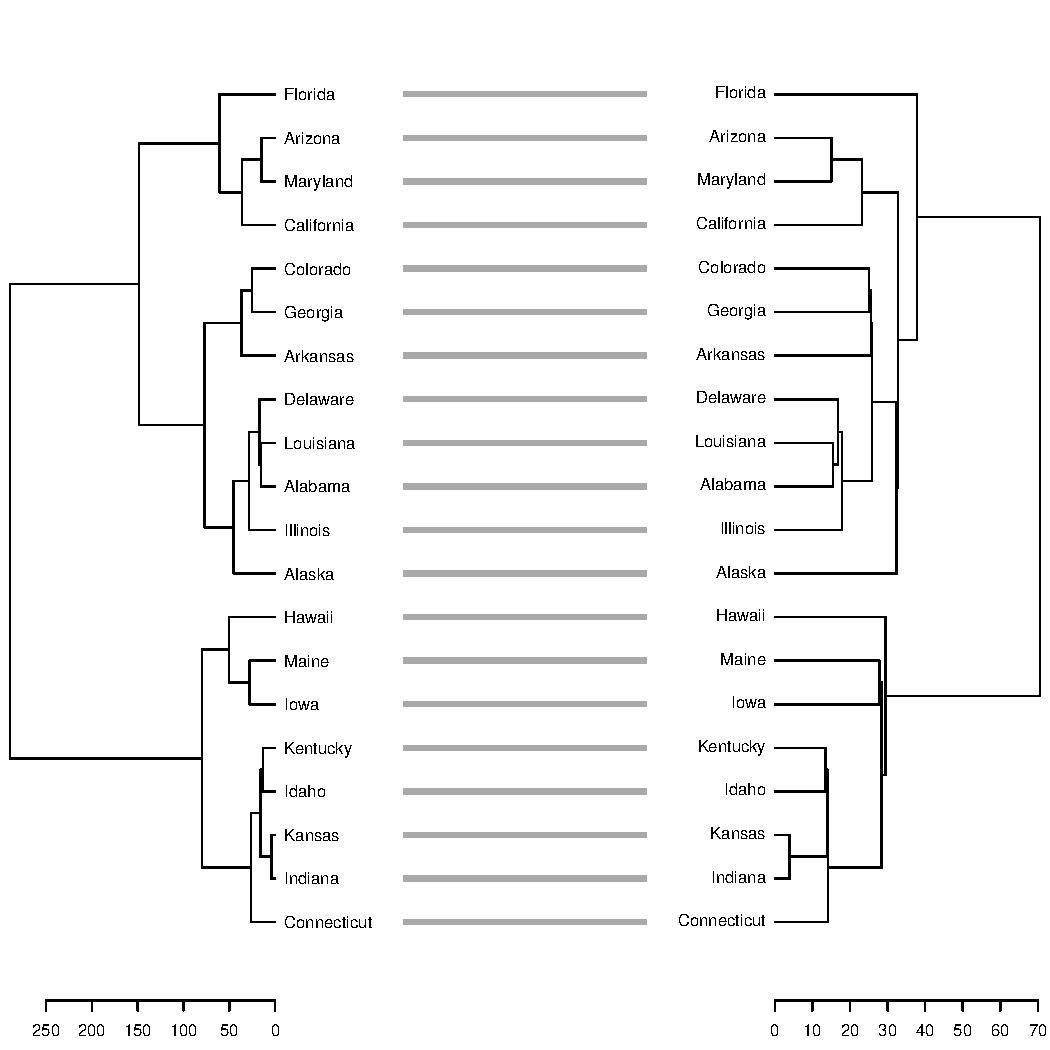
\includegraphics[width=\maxwidth]{figure/untangle_step_rotate_2side_example4} 

}


\begin{kframe}\begin{alltt}
\hlkwd{entanglement}\hlstd{(dend12_corrected_2[[}\hlnum{1}\hlstd{]], dend12_corrected_2[[}\hlnum{2}\hlstd{]],}
    \hlkwc{L} \hlstd{=} \hlnum{2}\hlstd{)}  \hlcom{# 0 - PERFECT.}
\end{alltt}
\begin{verbatim}
## [1] 0
\end{verbatim}
\begin{alltt}
\hlcom{# using rank_branches and k_branches, combined with type,}
\hlcom{# center, and xlim - helps to see various topological}
\hlcom{# differences between the two trees:}
\hlkwd{tanglegram}\hlstd{(dend12_corrected_2[[}\hlnum{1}\hlstd{]], dend12_corrected_2[[}\hlnum{2}\hlstd{]],}
    \hlkwc{k_branches} \hlstd{=} \hlnum{7}\hlstd{,} \hlkwc{rank_branches} \hlstd{=} \hlnum{TRUE}\hlstd{,} \hlkwc{margin_inner} \hlstd{=} \hlnum{6.5}\hlstd{,}
    \hlkwc{type} \hlstd{=} \hlstr{"t"}\hlstd{,} \hlkwc{center} \hlstd{=} \hlnum{TRUE}\hlstd{,} \hlkwc{xlim} \hlstd{=} \hlkwd{c}\hlstd{(}\hlnum{8}\hlstd{,} \hlnum{0}\hlstd{))}  \hlcom{# Much Better...}
\end{alltt}
\end{kframe}

{\centering 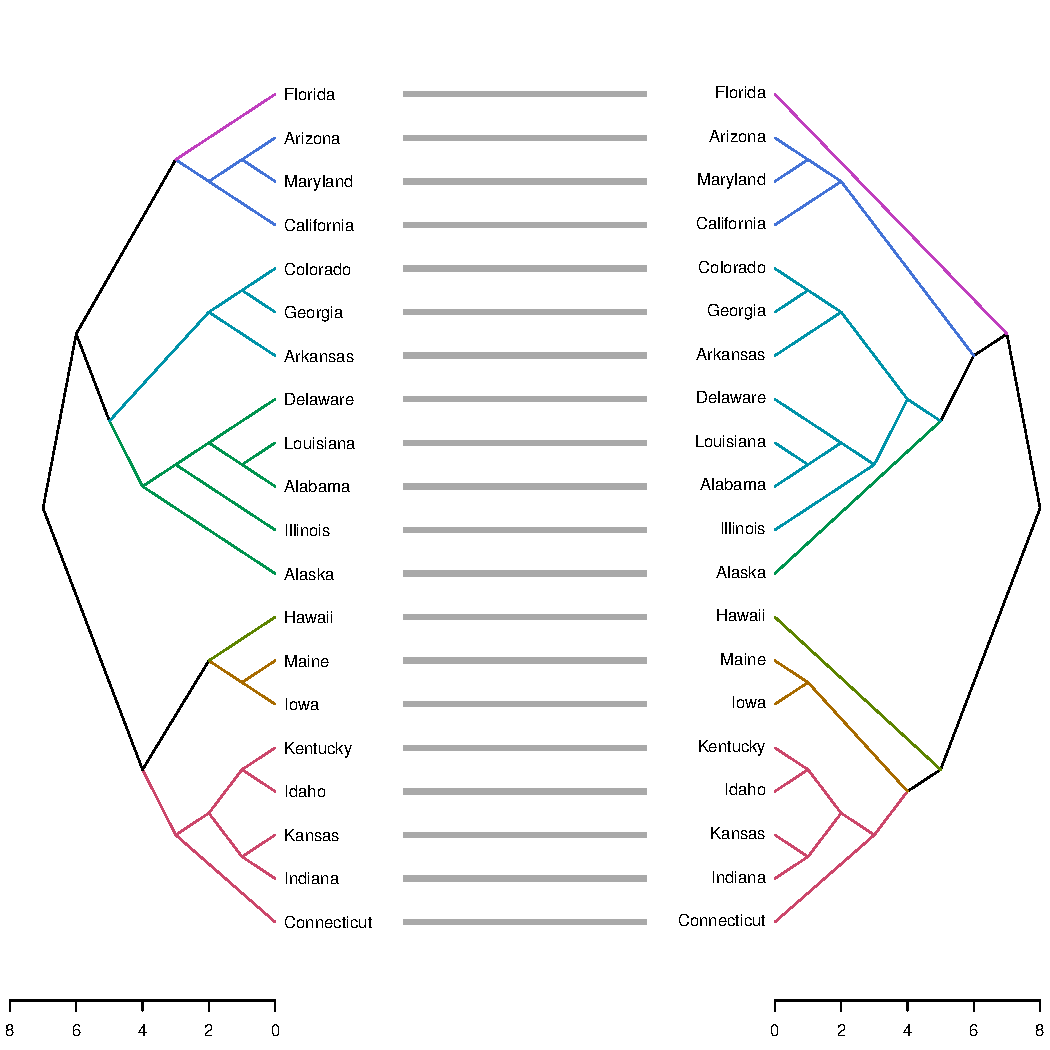
\includegraphics[width=\maxwidth]{figure/untangle_step_rotate_2side_example5} 

}


\begin{kframe}\begin{alltt}
\hlcom{# using 'hang=TRUE' also helps:}
\hlkwd{tanglegram}\hlstd{(dend12_corrected_2[[}\hlnum{1}\hlstd{]], dend12_corrected_2[[}\hlnum{2}\hlstd{]],}
    \hlkwc{k_branches} \hlstd{=} \hlnum{7}\hlstd{,} \hlkwc{rank_branches} \hlstd{=} \hlnum{TRUE}\hlstd{,} \hlkwc{hang} \hlstd{=} \hlnum{TRUE}\hlstd{,} \hlkwc{margin_inner} \hlstd{=} \hlnum{6.5}\hlstd{,}
    \hlkwc{type} \hlstd{=} \hlstr{"r"}\hlstd{,} \hlkwc{center} \hlstd{=} \hlnum{TRUE}\hlstd{,} \hlkwc{xlim} \hlstd{=} \hlkwd{c}\hlstd{(}\hlnum{8}\hlstd{,} \hlnum{0}\hlstd{))}  \hlcom{# Also Better... }
\end{alltt}
\end{kframe}

{\centering 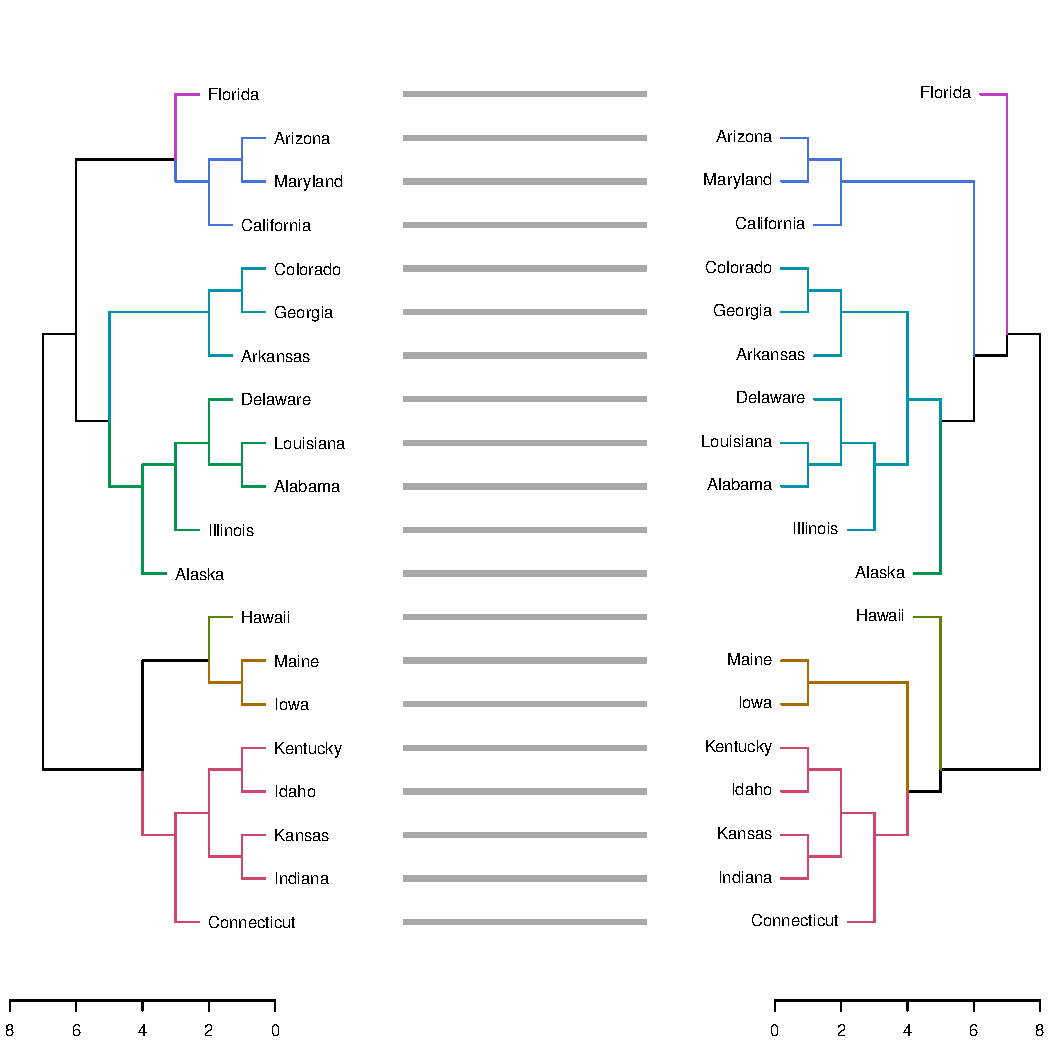
\includegraphics[width=\maxwidth]{figure/untangle_step_rotate_2side_example6} 

}


\begin{kframe}\begin{alltt}



\end{alltt}
\end{kframe}
\end{knitrout}





\section{Comparing two trees - statistics and inference}

\subsection{Baker's Gamma Index}

Baker's Gamma Index \citep{baker1974stability} is a measure of accosiation (similarity) 
between two trees of heirarchical clustering (dendrograms). It is defined as the rank correlation between the stages at which pairs of objects combine in each of the two trees.

Or more detailed: It is calculated by taking two items, and see what is the heighst
possible level of k (number of cluster groups created when cutting the tree)
for which the two item still belongs to the same tree. That k is returned, 
and the same is done for these two items for the second tree.
There are n over 2 combinations of such pairs of items from the items in 
the tree, and all of these numbers are calculated for each of the two trees. 
Then, these two sets of numbers (a set for the items in each tree)
are paired according to the pairs of items compared, and a spearman 
correlation is calculated.

The value can range between -1 to 1. With near 0 values meaning that
the two trees are not statistically similar.
For exact p-value one should result to a permutation test. One such option
will be to permute over the labels of one tree many times, and calculating 
the distriubtion under the null hypothesis (keeping the trees topologies
constant).

Notice that this measure is not affected by the height of a branch but only
of its relative position compared with other branches.


Here are a few examples:

\begin{knitrout}
\definecolor{shadecolor}{rgb}{0.969, 0.969, 0.969}\color{fgcolor}\begin{kframe}
\begin{alltt}
\hlkwd{set.seed}\hlstd{(}\hlnum{23235}\hlstd{)}
\hlstd{ss} \hlkwb{<-} \hlkwd{sample}\hlstd{(}\hlnum{1}\hlopt{:}\hlnum{150}\hlstd{,} \hlnum{10}\hlstd{)}  \hlcom{# we want to compare small trees}
\hlstd{hc1} \hlkwb{<-} \hlkwd{hclust}\hlstd{(}\hlkwd{dist}\hlstd{(iris[ss,} \hlopt{-}\hlnum{5}\hlstd{]),} \hlstr{"com"}\hlstd{)}
\hlstd{hc2} \hlkwb{<-} \hlkwd{hclust}\hlstd{(}\hlkwd{dist}\hlstd{(iris[ss,} \hlopt{-}\hlnum{5}\hlstd{]),} \hlstr{"single"}\hlstd{)}
\hlstd{dend1} \hlkwb{<-} \hlkwd{as.dendrogram}\hlstd{(hc1)}
\hlstd{dend2} \hlkwb{<-} \hlkwd{as.dendrogram}\hlstd{(hc2)}
\hlcom{# cutree(dend1)}

\hlkwd{cor_bakers_gamma}\hlstd{(hc1, hc2)}
\end{alltt}
\begin{verbatim}
## [1] 0.5716
\end{verbatim}
\begin{alltt}
\hlkwd{cor_bakers_gamma}\hlstd{(dend1, dend2)}
\end{alltt}
\begin{verbatim}
## [1] 0.5716
\end{verbatim}
\begin{alltt}
\hlcom{# dend1 <- match_order_by_labels(dend1, dend2) # if you are}
\hlcom{# not sure cor_bakers_gamma(dend1, dend2,}
\hlcom{# use_labels_not_values = FALSE)}

\hlkwd{require}\hlstd{(microbenchmark)}
\hlkwd{microbenchmark}\hlstd{(}\hlkwc{with_labels} \hlstd{=} \hlkwd{cor_bakers_gamma}\hlstd{(dend1, dend2,} \hlkwc{try_cutree_hclust} \hlstd{=} \hlnum{FALSE}\hlstd{),}
    \hlkwc{with_values} \hlstd{=} \hlkwd{cor_bakers_gamma}\hlstd{(dend1, dend2,} \hlkwc{use_labels_not_values} \hlstd{=} \hlnum{FALSE}\hlstd{,}
        \hlkwc{try_cutree_hclust} \hlstd{=} \hlnum{FALSE}\hlstd{),} \hlkwc{times} \hlstd{=} \hlnum{10}\hlstd{)}
\end{alltt}
\begin{verbatim}
## Unit: milliseconds
##         expr   min     lq median     uq    max neval
##  with_labels 97.98 101.87 103.83 105.58 111.81    10
##  with_values 84.62  87.63  89.64  92.06  92.97    10
\end{verbatim}
\begin{alltt}
\hlcom{# The cor of a tree with itself is 1:}
\hlkwd{cor_bakers_gamma}\hlstd{(dend1, dend1,} \hlkwc{use_labels_not_values} \hlstd{=} \hlnum{FALSE}\hlstd{)}
\end{alltt}
\begin{verbatim}
## [1] 1
\end{verbatim}
\begin{alltt}
\hlkwd{cor_bakers_gamma}\hlstd{(dend1, dend1,} \hlkwc{use_labels_not_values} \hlstd{=} \hlnum{TRUE}\hlstd{)}
\end{alltt}
\begin{verbatim}
## [1] 1
\end{verbatim}
\begin{alltt}
\hlkwd{entanglement}\hlstd{(dend1, dend1)}  \hlcom{# having a worse entanglement }
\end{alltt}
\begin{verbatim}
## [1] 0
\end{verbatim}
\begin{alltt}
\hlkwd{tanglegram}\hlstd{(dend1, dend1)}  \hlcom{# having a worse entanglement }
\end{alltt}
\end{kframe}

{\centering 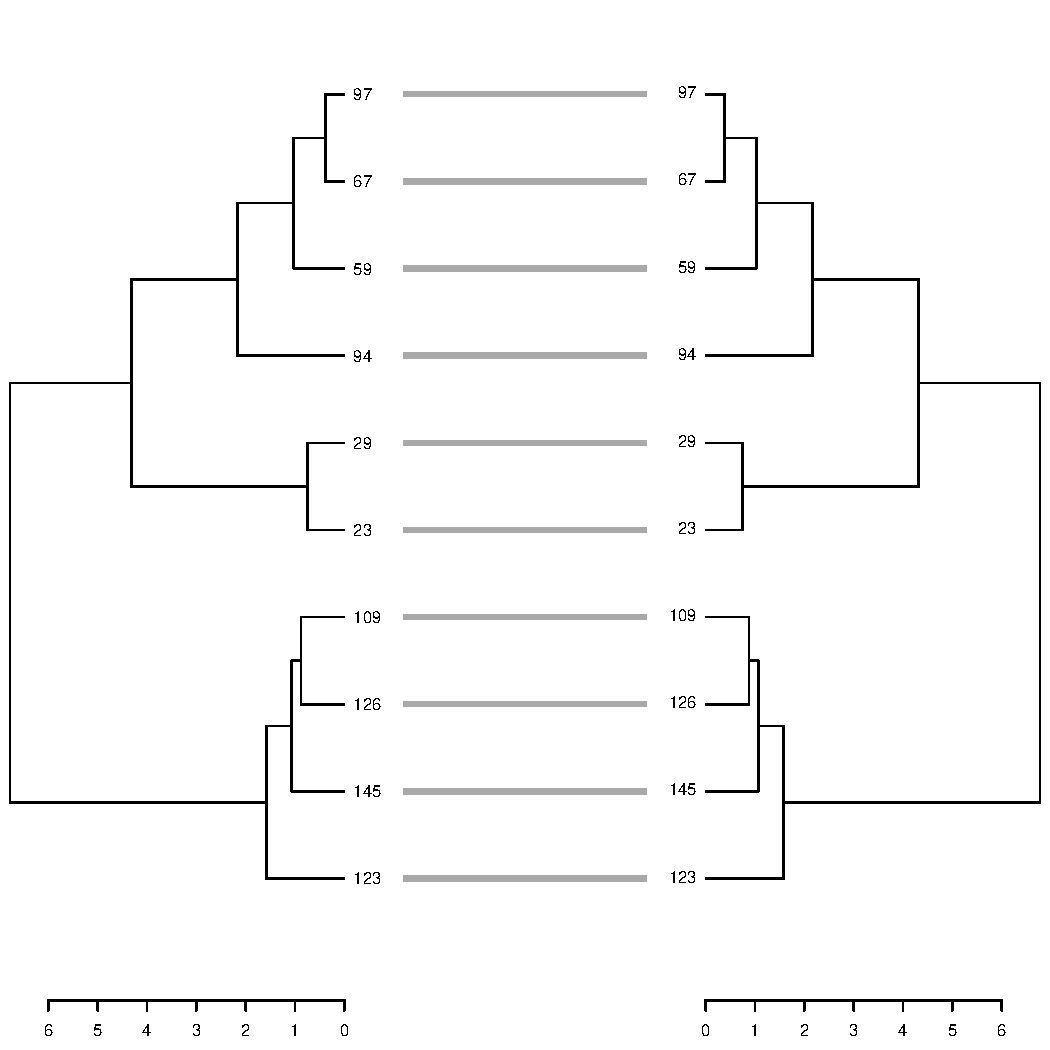
\includegraphics[width=\maxwidth]{figure/cor_bakers_gamma_example_11} 

}


\begin{kframe}\begin{alltt}
\hlcom{# tree order has no effect on the correlation:}
\hlstd{rev_dend1} \hlkwb{<-} \hlkwd{rev}\hlstd{(dend1)}
\hlkwd{cor_bakers_gamma}\hlstd{(dend1, rev_dend1,} \hlkwc{use_labels_not_values} \hlstd{=} \hlnum{TRUE}\hlstd{)}
\end{alltt}
\begin{verbatim}
## [1] 1
\end{verbatim}
\begin{alltt}
\hlkwd{entanglement}\hlstd{(dend1, rev_dend1)}  \hlcom{# having a worse entanglement }
\end{alltt}
\begin{verbatim}
## [1] 1
\end{verbatim}
\begin{alltt}
\hlkwd{tanglegram}\hlstd{(dend1, rev_dend1)}  \hlcom{# having a worse entanglement }
\end{alltt}
\end{kframe}

{\centering 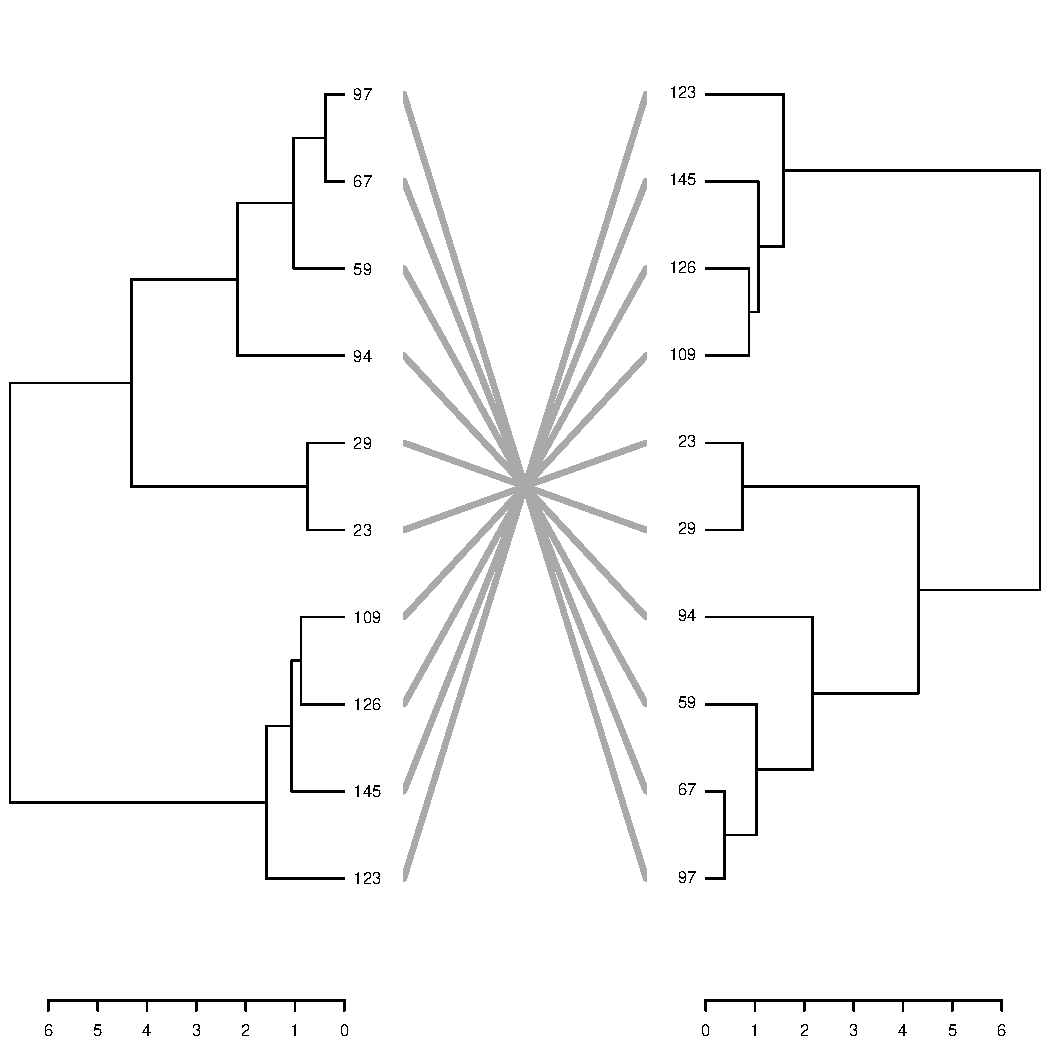
\includegraphics[width=\maxwidth]{figure/cor_bakers_gamma_example_12} 

}


\begin{kframe}\begin{alltt}
\hlcom{# But labels order does matter!!}
\hlstd{dend1_mixed} \hlkwb{<-} \hlstd{dend1}
\hlkwd{labels}\hlstd{(dend1_mixed)} \hlkwb{<-} \hlkwd{rev}\hlstd{(}\hlkwd{labels}\hlstd{(dend1_mixed))}
\hlkwd{tanglegram}\hlstd{(dend1, dend1_mixed)}
\end{alltt}
\end{kframe}

{\centering 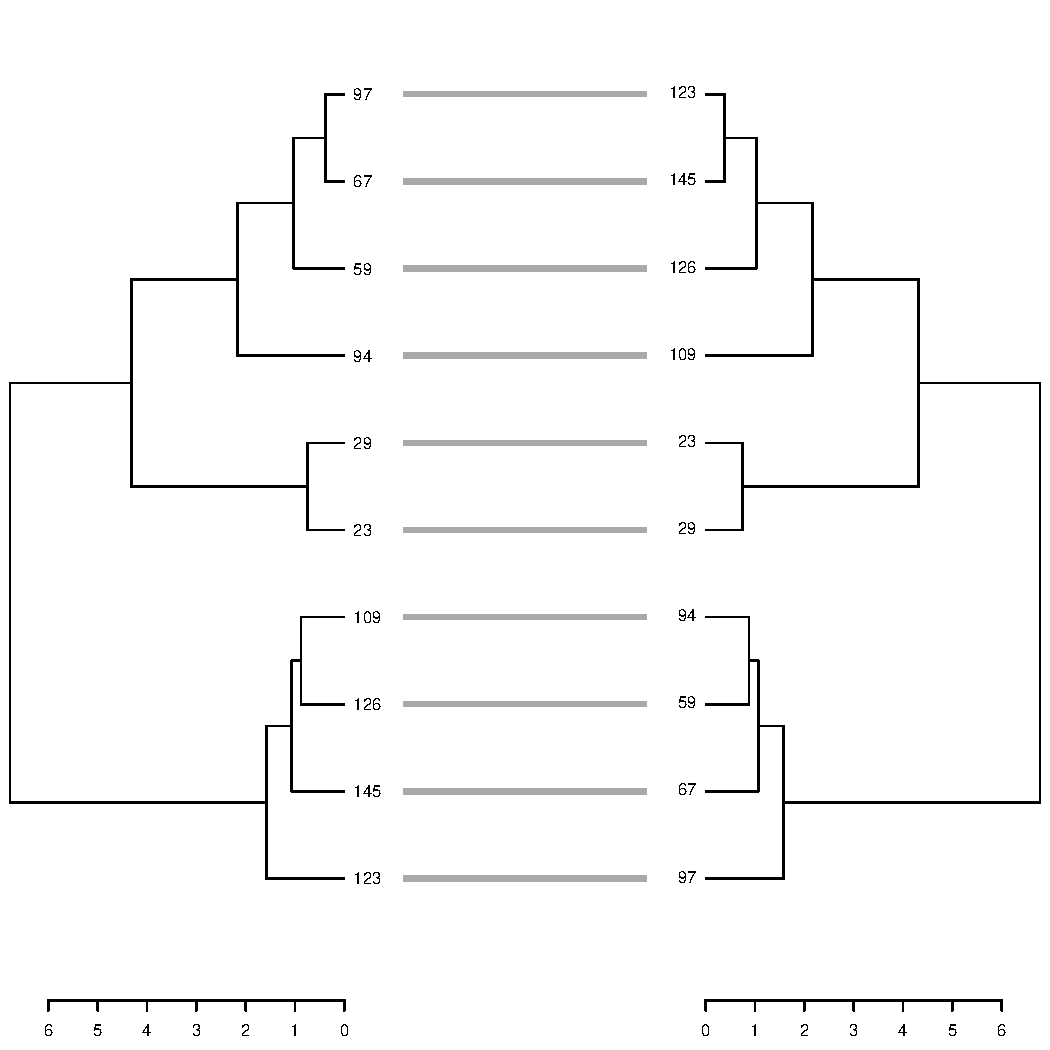
\includegraphics[width=\maxwidth]{figure/cor_bakers_gamma_example_13} 

}


\begin{kframe}\begin{alltt}
\hlkwd{entanglement}\hlstd{(dend1, dend1_mixed)}  \hlcom{# having the worst entanglement }
\end{alltt}
\begin{verbatim}
## [1] 1
\end{verbatim}
\begin{alltt}
\hlcom{# does NOT mean having the worst cor!}
\hlkwd{cor_bakers_gamma}\hlstd{(dend1, dend1_mixed,} \hlkwc{use_labels_not_values} \hlstd{=} \hlnum{TRUE}\hlstd{)}
\end{alltt}
\begin{verbatim}
## [1] 0.647
\end{verbatim}
\begin{alltt}
\hlkwd{set.seed}\hlstd{(}\hlnum{983597}\hlstd{)}
\hlkwd{labels}\hlstd{(dend1_mixed)} \hlkwb{<-} \hlkwd{sample}\hlstd{(}\hlkwd{labels}\hlstd{(dend1_mixed))}
\hlkwd{tanglegram}\hlstd{(dend1, dend1_mixed)}
\end{alltt}
\end{kframe}

{\centering 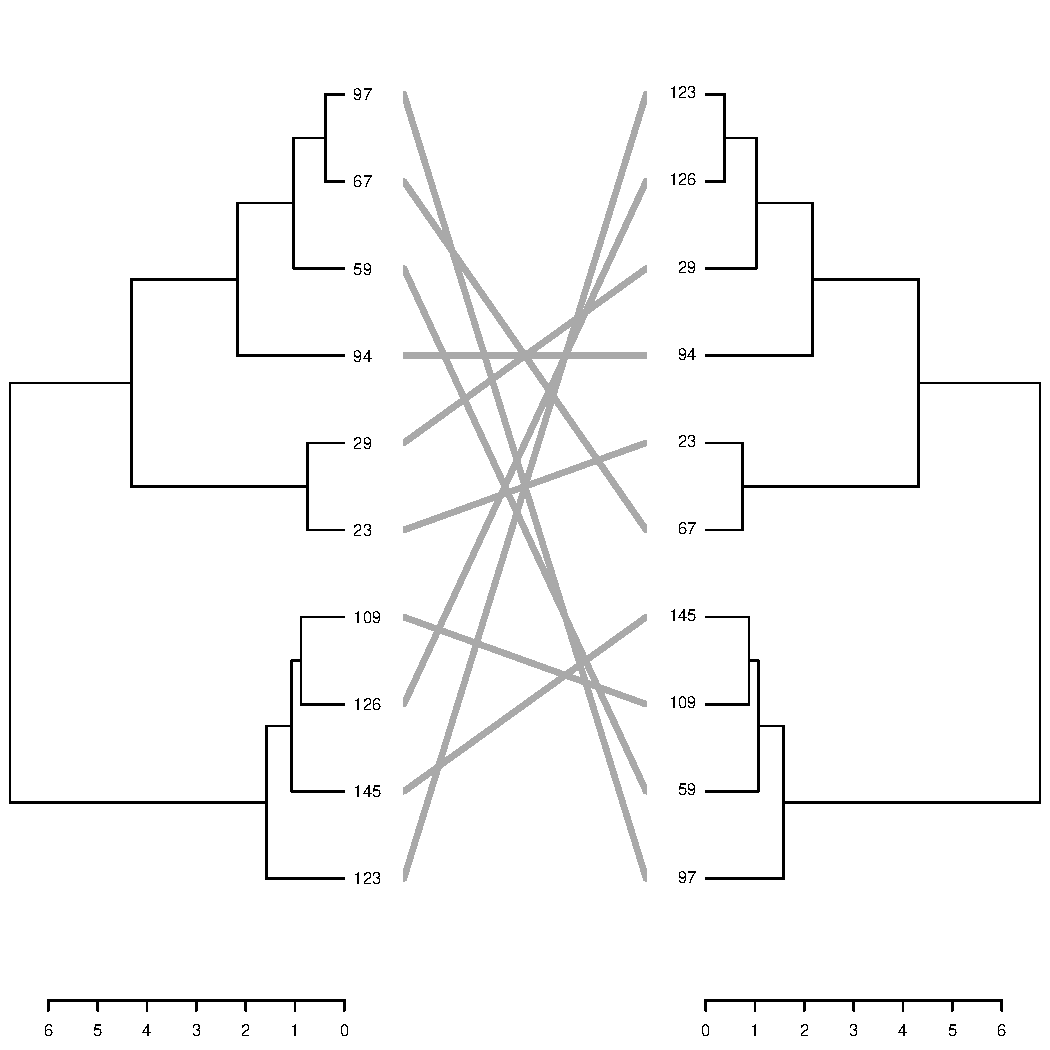
\includegraphics[width=\maxwidth]{figure/cor_bakers_gamma_example_14} 

}


\begin{kframe}\begin{alltt}
\hlkwd{entanglement}\hlstd{(dend1, dend1_mixed)}  \hlcom{# having a worse entanglement }
\end{alltt}
\begin{verbatim}
## [1] 0.7874
\end{verbatim}
\begin{alltt}
\hlkwd{cor_bakers_gamma}\hlstd{(dend1, dend1_mixed,} \hlkwc{use_labels_not_values} \hlstd{=} \hlnum{TRUE}\hlstd{)}
\end{alltt}
\begin{verbatim}
## [1] -0.06617
\end{verbatim}
\begin{alltt}

\end{alltt}
\end{kframe}
\end{knitrout}



Since the observations creating the Baker's Gamma Index of such a measure are correlated, we need to perform a permutation test for the calculation of the statistical significance of the index. Let's look at the distribution of Baker's Gamma Index under the null hypothesis (assuming fixed tree topologies). This will be different for different tree structures and sizes. Here are the results when the compared tree is itself (after shuffaling its own labels), and when comparing tree 1 to the shuffled tree 2:



\begin{knitrout}
\definecolor{shadecolor}{rgb}{0.969, 0.969, 0.969}\color{fgcolor}\begin{kframe}
\begin{alltt}
\hlkwd{set.seed}\hlstd{(}\hlnum{23235}\hlstd{)}
\hlstd{ss} \hlkwb{<-} \hlkwd{sample}\hlstd{(}\hlnum{1}\hlopt{:}\hlnum{150}\hlstd{,} \hlnum{10}\hlstd{)}  \hlcom{# we want to compare small trees}
\hlstd{hc1} \hlkwb{<-} \hlkwd{hclust}\hlstd{(}\hlkwd{dist}\hlstd{(iris[ss,} \hlopt{-}\hlnum{5}\hlstd{]),} \hlstr{"com"}\hlstd{)}
\hlstd{hc2} \hlkwb{<-} \hlkwd{hclust}\hlstd{(}\hlkwd{dist}\hlstd{(iris[ss,} \hlopt{-}\hlnum{5}\hlstd{]),} \hlstr{"single"}\hlstd{)}
\hlstd{dend1} \hlkwb{<-} \hlkwd{as.dendrogram}\hlstd{(hc1)}
\hlstd{dend2} \hlkwb{<-} \hlkwd{as.dendrogram}\hlstd{(hc2)}
\hlcom{# cutree(dend1)}

\hlstd{the_cor} \hlkwb{<-} \hlkwd{cor_bakers_gamma}\hlstd{(dend1, dend1)}
\hlstd{the_cor}
\end{alltt}
\begin{verbatim}
## [1] 1
\end{verbatim}
\begin{alltt}
\hlstd{R} \hlkwb{<-} \hlnum{1000}
\hlstd{cor_bakers_gamma_results} \hlkwb{<-} \hlkwd{numeric}\hlstd{(R)}
\hlstd{dend_mixed} \hlkwb{<-} \hlstd{dend1}
\hlkwa{for} \hlstd{(i} \hlkwa{in} \hlnum{1}\hlopt{:}\hlstd{R) \{}
    \hlstd{dend_mixed} \hlkwb{<-} \hlkwd{sample.dendrogram}\hlstd{(dend_mixed,} \hlkwc{replace} \hlstd{=} \hlnum{FALSE}\hlstd{)}
    \hlstd{cor_bakers_gamma_results[i]} \hlkwb{<-} \hlkwd{cor_bakers_gamma}\hlstd{(dend1, dend_mixed)}
\hlstd{\}}
\hlkwd{plot}\hlstd{(}\hlkwd{density}\hlstd{(cor_bakers_gamma_results),} \hlkwc{main} \hlstd{=} \hlstr{"Baker's gamma distribution under H0"}\hlstd{,}
    \hlkwc{xlim} \hlstd{=} \hlkwd{c}\hlstd{(}\hlopt{-}\hlnum{1}\hlstd{,} \hlnum{1}\hlstd{))}
\hlkwd{abline}\hlstd{(}\hlkwc{v} \hlstd{=} \hlnum{0}\hlstd{,} \hlkwc{lty} \hlstd{=} \hlnum{2}\hlstd{)}
\hlkwd{abline}\hlstd{(}\hlkwc{v} \hlstd{= the_cor,} \hlkwc{lty} \hlstd{=} \hlnum{2}\hlstd{,} \hlkwc{col} \hlstd{=} \hlnum{2}\hlstd{)}
\hlkwd{title}\hlstd{(}\hlkwc{sub} \hlstd{=} \hlkwd{paste}\hlstd{(}\hlstr{"One sided p-value ="}\hlstd{,} \hlkwd{round}\hlstd{(}\hlkwd{sum}\hlstd{(the_cor} \hlopt{<}
    \hlstd{cor_bakers_gamma_results)}\hlopt{/}\hlstd{R,} \hlnum{4}\hlstd{)))}
\end{alltt}
\end{kframe}

{\centering 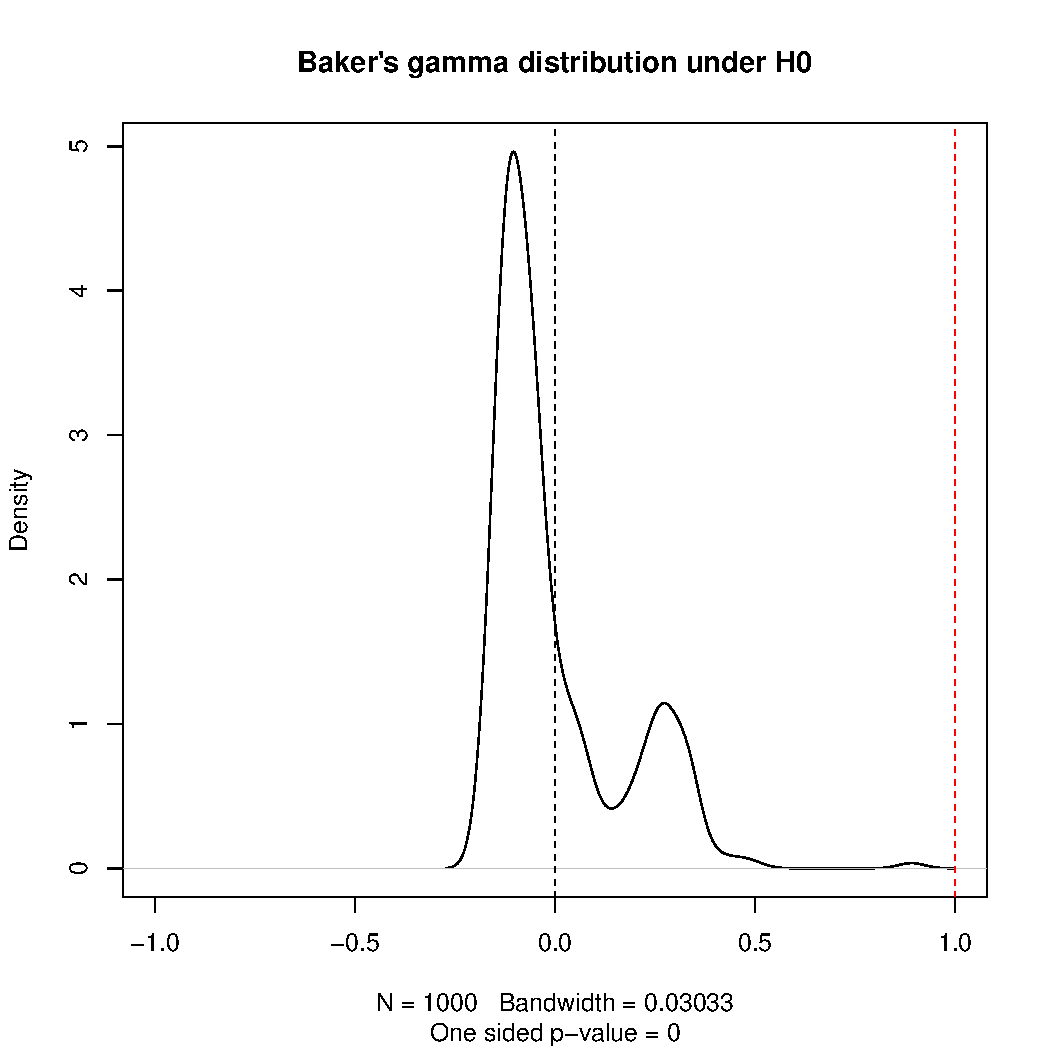
\includegraphics[width=\maxwidth]{figure/cor_bakers_gamma_simulation_1} 

}



\end{knitrout}



\begin{knitrout}
\definecolor{shadecolor}{rgb}{0.969, 0.969, 0.969}\color{fgcolor}\begin{kframe}
\begin{alltt}
\hlkwd{set.seed}\hlstd{(}\hlnum{23235}\hlstd{)}
\hlstd{ss} \hlkwb{<-} \hlkwd{sample}\hlstd{(}\hlnum{1}\hlopt{:}\hlnum{150}\hlstd{,} \hlnum{10}\hlstd{)}  \hlcom{# we want to compare small trees}
\hlstd{hc1} \hlkwb{<-} \hlkwd{hclust}\hlstd{(}\hlkwd{dist}\hlstd{(iris[ss,} \hlopt{-}\hlnum{5}\hlstd{]),} \hlstr{"com"}\hlstd{)}
\hlstd{hc2} \hlkwb{<-} \hlkwd{hclust}\hlstd{(}\hlkwd{dist}\hlstd{(iris[ss,} \hlopt{-}\hlnum{5}\hlstd{]),} \hlstr{"single"}\hlstd{)}
\hlstd{dend1} \hlkwb{<-} \hlkwd{as.dendrogram}\hlstd{(hc1)}
\hlstd{dend2} \hlkwb{<-} \hlkwd{as.dendrogram}\hlstd{(hc2)}
\hlcom{# cutree(dend1)}

\hlstd{the_cor} \hlkwb{<-} \hlkwd{cor_bakers_gamma}\hlstd{(dend1, dend2)}
\hlstd{the_cor}
\end{alltt}
\begin{verbatim}
## [1] 0.5716
\end{verbatim}
\begin{alltt}
\hlstd{R} \hlkwb{<-} \hlnum{1000}
\hlstd{cor_bakers_gamma_results} \hlkwb{<-} \hlkwd{numeric}\hlstd{(R)}
\hlstd{dend_mixed} \hlkwb{<-} \hlstd{dend2}
\hlkwa{for} \hlstd{(i} \hlkwa{in} \hlnum{1}\hlopt{:}\hlstd{R) \{}
    \hlstd{dend_mixed} \hlkwb{<-} \hlkwd{sample.dendrogram}\hlstd{(dend_mixed,} \hlkwc{replace} \hlstd{=} \hlnum{FALSE}\hlstd{)}
    \hlstd{cor_bakers_gamma_results[i]} \hlkwb{<-} \hlkwd{cor_bakers_gamma}\hlstd{(dend1, dend_mixed)}
\hlstd{\}}
\hlkwd{plot}\hlstd{(}\hlkwd{density}\hlstd{(cor_bakers_gamma_results),} \hlkwc{main} \hlstd{=} \hlstr{"Baker's gamma distribution under H0"}\hlstd{,}
    \hlkwc{xlim} \hlstd{=} \hlkwd{c}\hlstd{(}\hlopt{-}\hlnum{1}\hlstd{,} \hlnum{1}\hlstd{))}
\hlkwd{abline}\hlstd{(}\hlkwc{v} \hlstd{=} \hlnum{0}\hlstd{,} \hlkwc{lty} \hlstd{=} \hlnum{2}\hlstd{)}
\hlkwd{abline}\hlstd{(}\hlkwc{v} \hlstd{= the_cor,} \hlkwc{lty} \hlstd{=} \hlnum{2}\hlstd{,} \hlkwc{col} \hlstd{=} \hlnum{2}\hlstd{)}
\hlkwd{title}\hlstd{(}\hlkwc{sub} \hlstd{=} \hlkwd{paste}\hlstd{(}\hlstr{"One sided p-value ="}\hlstd{,} \hlkwd{round}\hlstd{(}\hlkwd{sum}\hlstd{(the_cor} \hlopt{<}
    \hlstd{cor_bakers_gamma_results)}\hlopt{/}\hlstd{R,} \hlnum{4}\hlstd{)))}
\end{alltt}
\end{kframe}

{\centering 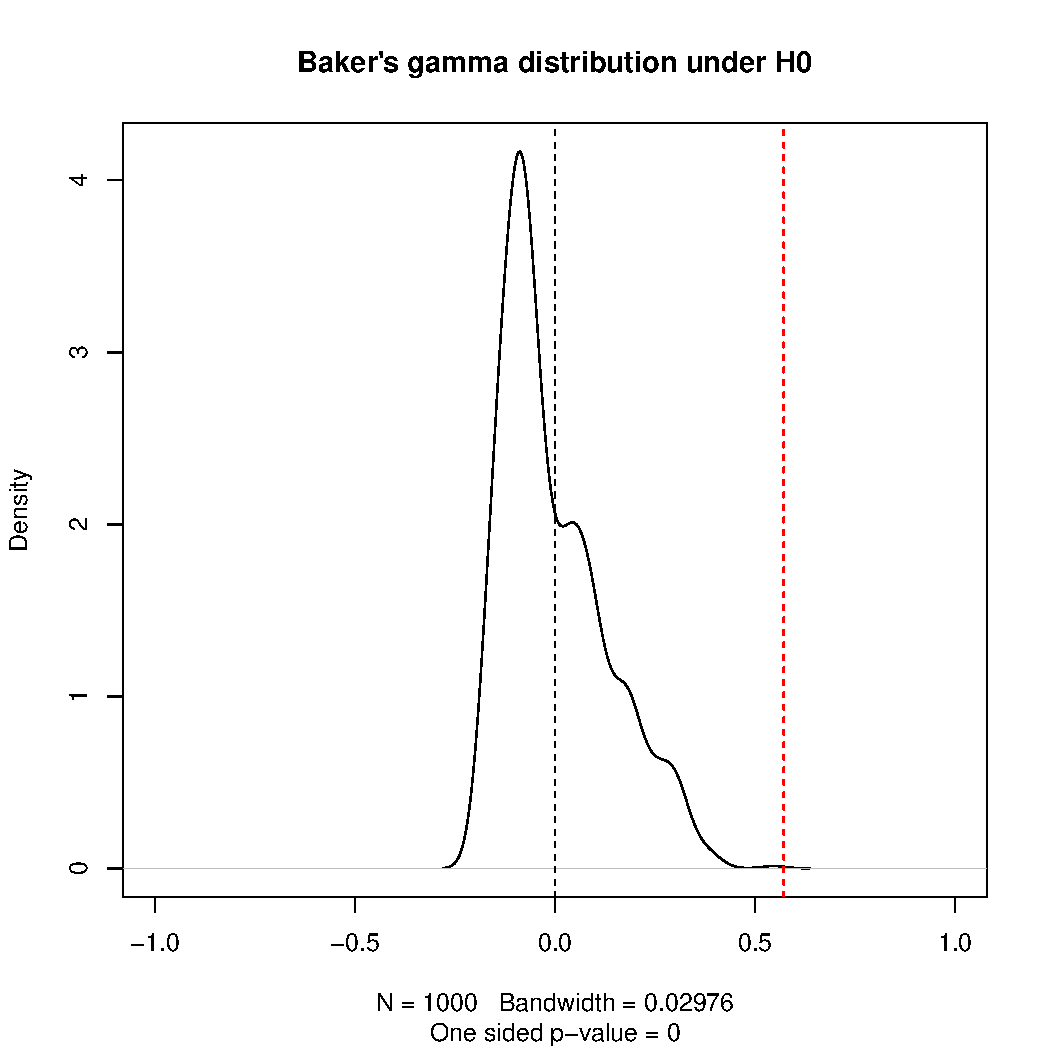
\includegraphics[width=\maxwidth]{figure/cor_bakers_gamma_simulation_2} 

}



\end{knitrout}



And lastly, let us look at a simulation were labels of both trees are shuffled:


\begin{knitrout}
\definecolor{shadecolor}{rgb}{0.969, 0.969, 0.969}\color{fgcolor}\begin{kframe}
\begin{alltt}
\hlkwd{set.seed}\hlstd{(}\hlnum{23235}\hlstd{)}
\hlstd{ss} \hlkwb{<-} \hlkwd{sample}\hlstd{(}\hlnum{1}\hlopt{:}\hlnum{150}\hlstd{,} \hlnum{10}\hlstd{)}  \hlcom{# we want to compare small trees}
\hlstd{hc1} \hlkwb{<-} \hlkwd{hclust}\hlstd{(}\hlkwd{dist}\hlstd{(iris[ss,} \hlopt{-}\hlnum{5}\hlstd{]),} \hlstr{"com"}\hlstd{)}
\hlstd{hc2} \hlkwb{<-} \hlkwd{hclust}\hlstd{(}\hlkwd{dist}\hlstd{(iris[ss,} \hlopt{-}\hlnum{5}\hlstd{]),} \hlstr{"single"}\hlstd{)}
\hlstd{dend1} \hlkwb{<-} \hlkwd{as.dendrogram}\hlstd{(hc1)}
\hlstd{dend2} \hlkwb{<-} \hlkwd{as.dendrogram}\hlstd{(hc2)}
\hlcom{# cutree(dend1)}

\hlstd{the_cor} \hlkwb{<-} \hlkwd{cor_bakers_gamma}\hlstd{(dend1, dend2)}
\hlstd{the_cor}
\end{alltt}
\begin{verbatim}
## [1] 0.5716
\end{verbatim}
\begin{alltt}
\hlstd{R} \hlkwb{<-} \hlnum{1000}
\hlstd{cor_bakers_gamma_results} \hlkwb{<-} \hlkwd{numeric}\hlstd{(R)}
\hlstd{dend_mixed1} \hlkwb{<-} \hlstd{dend1}
\hlstd{dend_mixed2} \hlkwb{<-} \hlstd{dend2}
\hlkwa{for} \hlstd{(i} \hlkwa{in} \hlnum{1}\hlopt{:}\hlstd{R) \{}
    \hlstd{dend_mixed1} \hlkwb{<-} \hlkwd{sample.dendrogram}\hlstd{(dend_mixed1,} \hlkwc{replace} \hlstd{=} \hlnum{FALSE}\hlstd{)}
    \hlstd{dend_mixed2} \hlkwb{<-} \hlkwd{sample.dendrogram}\hlstd{(dend_mixed2,} \hlkwc{replace} \hlstd{=} \hlnum{FALSE}\hlstd{)}
    \hlstd{cor_bakers_gamma_results[i]} \hlkwb{<-} \hlkwd{cor_bakers_gamma}\hlstd{(dend_mixed1,}
        \hlstd{dend_mixed2)}
\hlstd{\}}
\hlkwd{plot}\hlstd{(}\hlkwd{density}\hlstd{(cor_bakers_gamma_results),} \hlkwc{main} \hlstd{=} \hlstr{"Baker's gamma distribution under H0"}\hlstd{,}
    \hlkwc{xlim} \hlstd{=} \hlkwd{c}\hlstd{(}\hlopt{-}\hlnum{1}\hlstd{,} \hlnum{1}\hlstd{))}
\hlkwd{abline}\hlstd{(}\hlkwc{v} \hlstd{=} \hlnum{0}\hlstd{,} \hlkwc{lty} \hlstd{=} \hlnum{2}\hlstd{)}
\hlkwd{abline}\hlstd{(}\hlkwc{v} \hlstd{= the_cor,} \hlkwc{lty} \hlstd{=} \hlnum{2}\hlstd{,} \hlkwc{col} \hlstd{=} \hlnum{2}\hlstd{)}
\hlkwd{title}\hlstd{(}\hlkwc{sub} \hlstd{=} \hlkwd{paste}\hlstd{(}\hlstr{"One sided p-value ="}\hlstd{,} \hlkwd{round}\hlstd{(}\hlkwd{sum}\hlstd{(the_cor} \hlopt{<}
    \hlstd{cor_bakers_gamma_results)}\hlopt{/}\hlstd{R,} \hlnum{4}\hlstd{)))}
\end{alltt}
\end{kframe}

{\centering 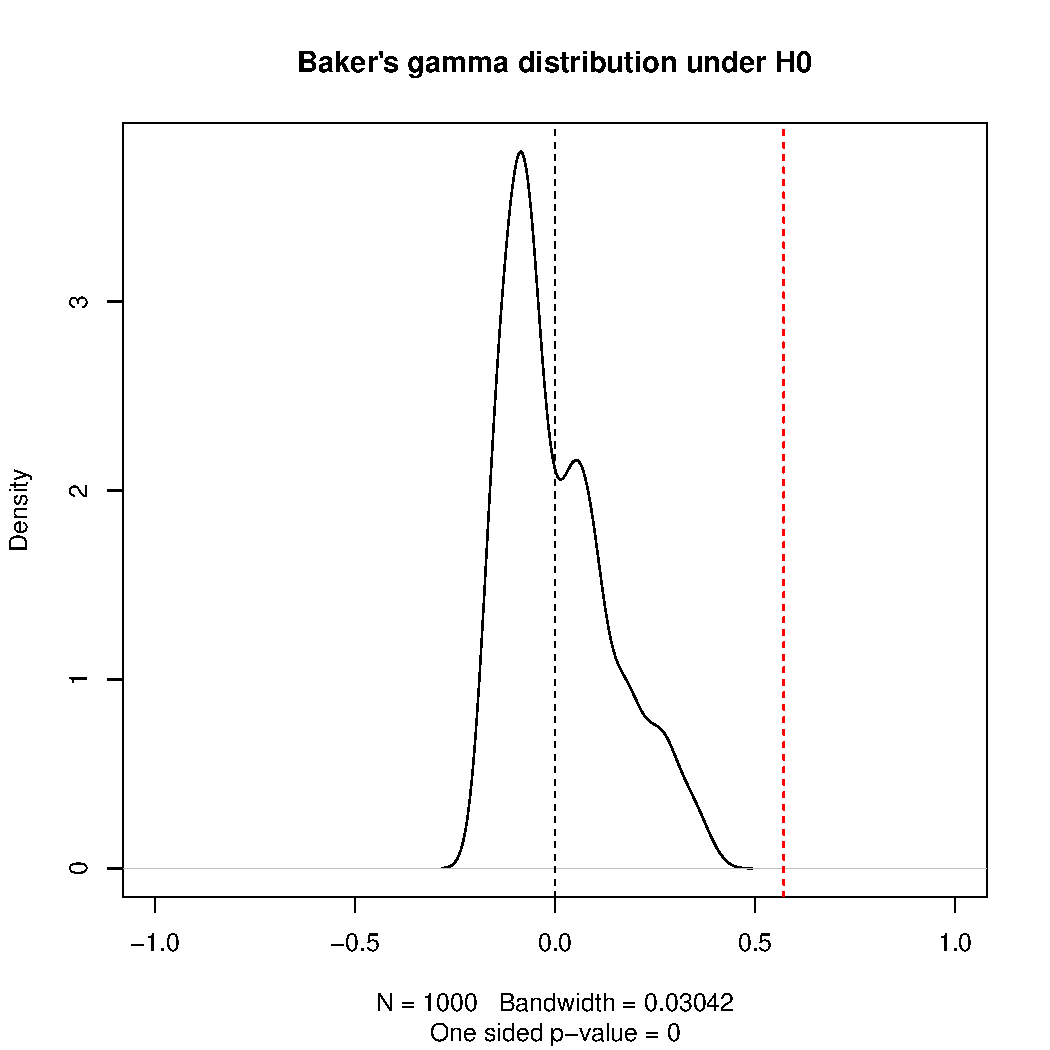
\includegraphics[width=\maxwidth]{figure/cor_bakers_gamma_simulation_3} 

}



\end{knitrout}


We can also calculate a bootstrap confidence interval using the \code{sample.dendrogram} function. This function can be very slow for larger trees, so make sure you use if carefully:

\begin{knitrout}
\definecolor{shadecolor}{rgb}{0.969, 0.969, 0.969}\color{fgcolor}\begin{kframe}
\begin{alltt}
\hlkwd{set.seed}\hlstd{(}\hlnum{312356}\hlstd{)}
\hlstd{ss} \hlkwb{<-} \hlkwd{sample}\hlstd{(}\hlnum{1}\hlopt{:}\hlnum{150}\hlstd{,} \hlnum{10}\hlstd{)}  \hlcom{# we want to compare small trees}
\hlstd{hc1} \hlkwb{<-} \hlkwd{hclust}\hlstd{(}\hlkwd{dist}\hlstd{(iris[ss,} \hlopt{-}\hlnum{5}\hlstd{]),} \hlstr{"com"}\hlstd{)}
\hlstd{hc2} \hlkwb{<-} \hlkwd{hclust}\hlstd{(}\hlkwd{dist}\hlstd{(iris[ss,} \hlopt{-}\hlnum{5}\hlstd{]),} \hlstr{"single"}\hlstd{)}
\hlstd{dend1} \hlkwb{<-} \hlkwd{as.dendrogram}\hlstd{(hc1)}
\hlstd{dend2} \hlkwb{<-} \hlkwd{as.dendrogram}\hlstd{(hc2)}
\hlcom{# tanglegram(dend1, dend2) cutree(dend1)}

\hlstd{R} \hlkwb{<-} \hlnum{1000}
\hlstd{dend1_labels} \hlkwb{<-} \hlkwd{labels}\hlstd{(dend1)}
\hlstd{dend2_labels} \hlkwb{<-} \hlkwd{labels}\hlstd{(dend2)}
\hlstd{cor_bakers_gamma_results} \hlkwb{<-} \hlkwd{numeric}\hlstd{(R)}
\hlkwa{for} \hlstd{(i} \hlkwa{in} \hlnum{1}\hlopt{:}\hlstd{R) \{}
    \hlstd{sampled_labels} \hlkwb{<-} \hlkwd{sample}\hlstd{(dend1_labels,} \hlkwc{replace} \hlstd{=} \hlnum{TRUE}\hlstd{)}
    \hlcom{# members needs to be fixed since it will be later used in}
    \hlcom{# nleaves}
    \hlstd{dend_mixed1} \hlkwb{<-} \hlkwd{sample.dendrogram}\hlstd{(dend1,} \hlkwc{dend_labels} \hlstd{= dend1_labels,}
        \hlkwc{fix_members} \hlstd{=} \hlnum{TRUE}\hlstd{,} \hlkwc{fix_order} \hlstd{=} \hlnum{TRUE}\hlstd{,} \hlkwc{fix_midpoint} \hlstd{=} \hlnum{FALSE}\hlstd{,}
        \hlkwc{replace} \hlstd{=} \hlnum{TRUE}\hlstd{,} \hlkwc{sampled_labels} \hlstd{= sampled_labels)}
    \hlstd{dend_mixed2} \hlkwb{<-} \hlkwd{sample.dendrogram}\hlstd{(dend2,} \hlkwc{dend_labels} \hlstd{= dend2_labels,}
        \hlkwc{fix_members} \hlstd{=} \hlnum{TRUE}\hlstd{,} \hlkwc{fix_order} \hlstd{=} \hlnum{TRUE}\hlstd{,} \hlkwc{fix_midpoint} \hlstd{=} \hlnum{FALSE}\hlstd{,}
        \hlkwc{replace} \hlstd{=} \hlnum{TRUE}\hlstd{,} \hlkwc{sampled_labels} \hlstd{= sampled_labels)}
    \hlstd{cor_bakers_gamma_results[i]} \hlkwb{<-} \hlkwd{cor_bakers_gamma}\hlstd{(dend_mixed1,}
        \hlstd{dend_mixed2,} \hlkwc{warn} \hlstd{=} \hlnum{FALSE}\hlstd{)}
\hlstd{\}}


\hlcom{# here is the tanglegram}
\hlkwd{tanglegram}\hlstd{(dend1, dend2)}
\end{alltt}
\end{kframe}

{\centering 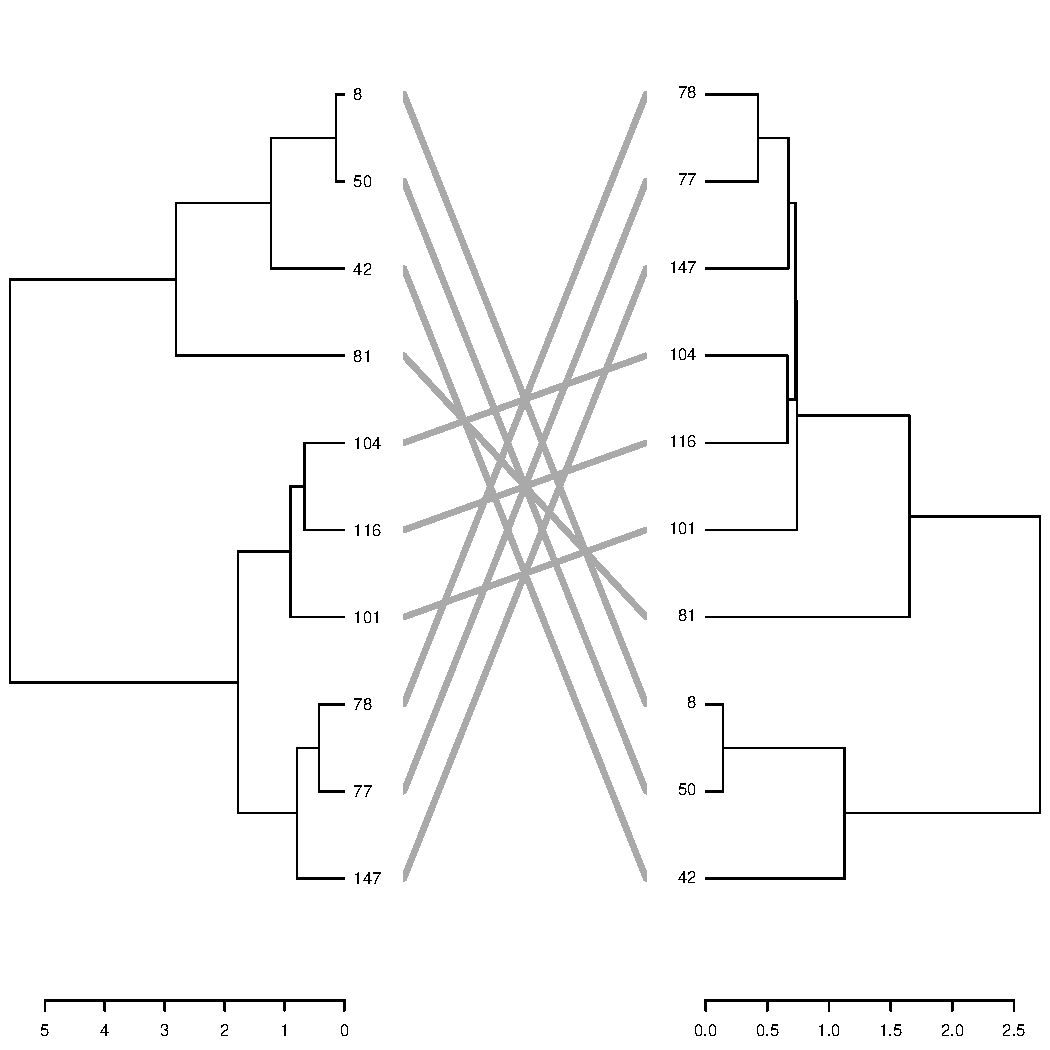
\includegraphics[width=\maxwidth]{figure/cor_bakers_gamma_simulation_CI_41} 

}


\begin{kframe}\begin{alltt}
\hlcom{# And here is the tanglegram for one sample of our trees:}
\hlstd{dend_mixed1} \hlkwb{<-} \hlkwd{rank_order.dendrogram}\hlstd{(dend_mixed1)}
\hlstd{dend_mixed2} \hlkwb{<-} \hlkwd{rank_order.dendrogram}\hlstd{(dend_mixed2)}
\hlstd{dend_mixed1} \hlkwb{<-} \hlkwd{fix_members_attr.dendrogram}\hlstd{(dend_mixed1)}
\hlstd{dend_mixed2} \hlkwb{<-} \hlkwd{fix_members_attr.dendrogram}\hlstd{(dend_mixed2)}
\hlkwd{tanglegram}\hlstd{(dend_mixed1, dend_mixed2)}
\end{alltt}
\end{kframe}

{\centering 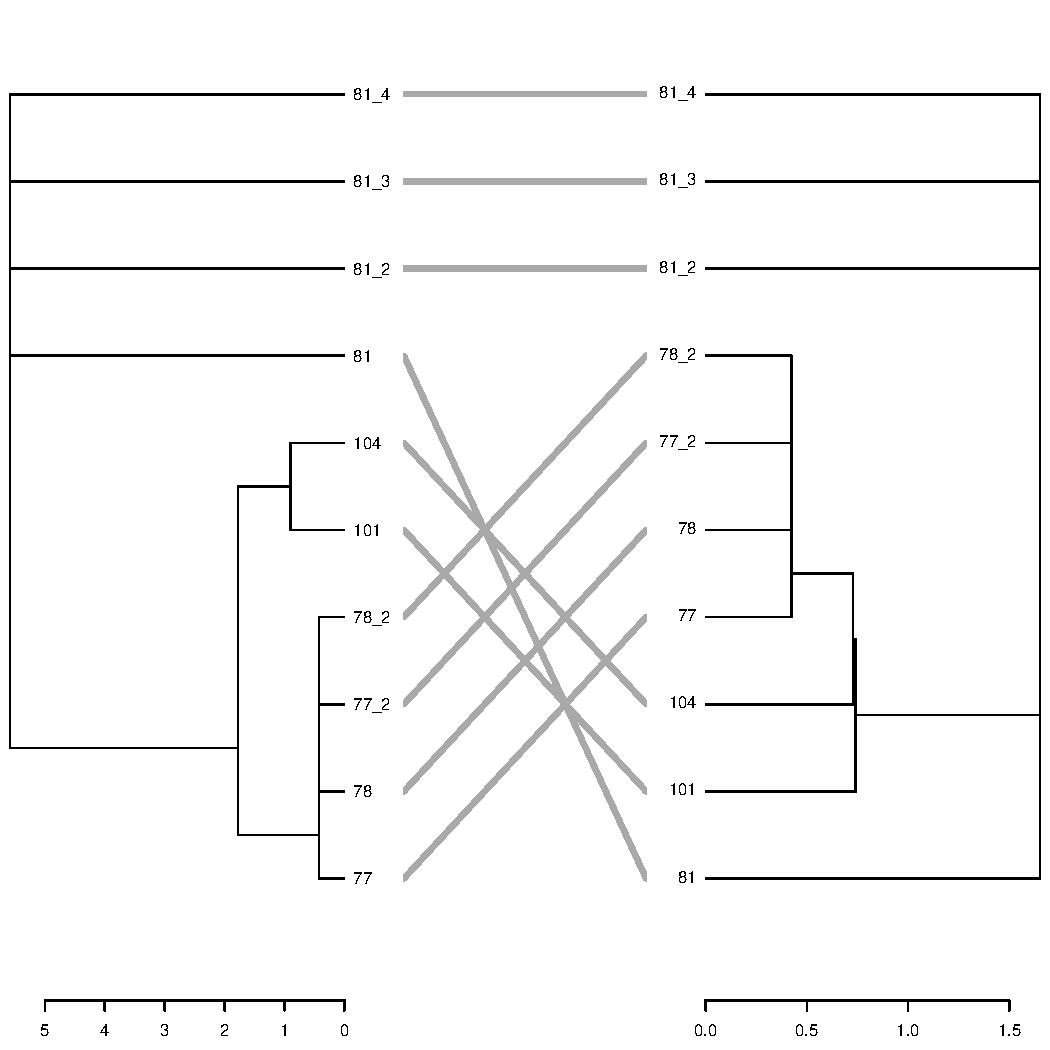
\includegraphics[width=\maxwidth]{figure/cor_bakers_gamma_simulation_CI_42} 

}


\begin{kframe}\begin{alltt}
\hlkwd{cor_bakers_gamma}\hlstd{(dend_mixed1, dend_mixed2,} \hlkwc{warn} \hlstd{=} \hlnum{FALSE}\hlstd{)}
\end{alltt}
\begin{verbatim}
## [1] 0.9924
\end{verbatim}
\begin{alltt}
\hlstd{CI95} \hlkwb{<-} \hlkwd{quantile}\hlstd{(cor_bakers_gamma_results,} \hlkwc{probs} \hlstd{=} \hlkwd{c}\hlstd{(}\hlnum{0.025}\hlstd{,} \hlnum{0.975}\hlstd{))}
\hlstd{CI95}
\end{alltt}
\begin{verbatim}
##   2.5%  97.5% 
## 0.4674 1.0000
\end{verbatim}
\begin{alltt}
\hlkwd{par}\hlstd{(}\hlkwc{mfrow} \hlstd{=} \hlkwd{c}\hlstd{(}\hlnum{1}\hlstd{,} \hlnum{1}\hlstd{))}
\hlkwd{plot}\hlstd{(}\hlkwd{density}\hlstd{(cor_bakers_gamma_results),} \hlkwc{main} \hlstd{=} \hlstr{"Baker's gamma bootstrap distribution"}\hlstd{,}
    \hlkwc{xlim} \hlstd{=} \hlkwd{c}\hlstd{(}\hlopt{-}\hlnum{1}\hlstd{,} \hlnum{1}\hlstd{))}
\hlkwd{abline}\hlstd{(}\hlkwc{v} \hlstd{= CI95,} \hlkwc{lty} \hlstd{=} \hlnum{2}\hlstd{,} \hlkwc{col} \hlstd{=} \hlnum{3}\hlstd{)}
\hlkwd{abline}\hlstd{(}\hlkwc{v} \hlstd{=} \hlkwd{cor_bakers_gamma}\hlstd{(dend1, dend2),} \hlkwc{lty} \hlstd{=} \hlnum{2}\hlstd{,} \hlkwc{col} \hlstd{=} \hlnum{2}\hlstd{)}
\hlkwd{legend}\hlstd{(}\hlstr{"topleft"}\hlstd{,} \hlkwc{legend} \hlstd{=} \hlkwd{c}\hlstd{(}\hlstr{"95% CI"}\hlstd{,} \hlstr{"Baker's Gamma Index"}\hlstd{),}
    \hlkwc{fill} \hlstd{=} \hlkwd{c}\hlstd{(}\hlnum{3}\hlstd{,} \hlnum{2}\hlstd{))}
\end{alltt}
\end{kframe}

{\centering 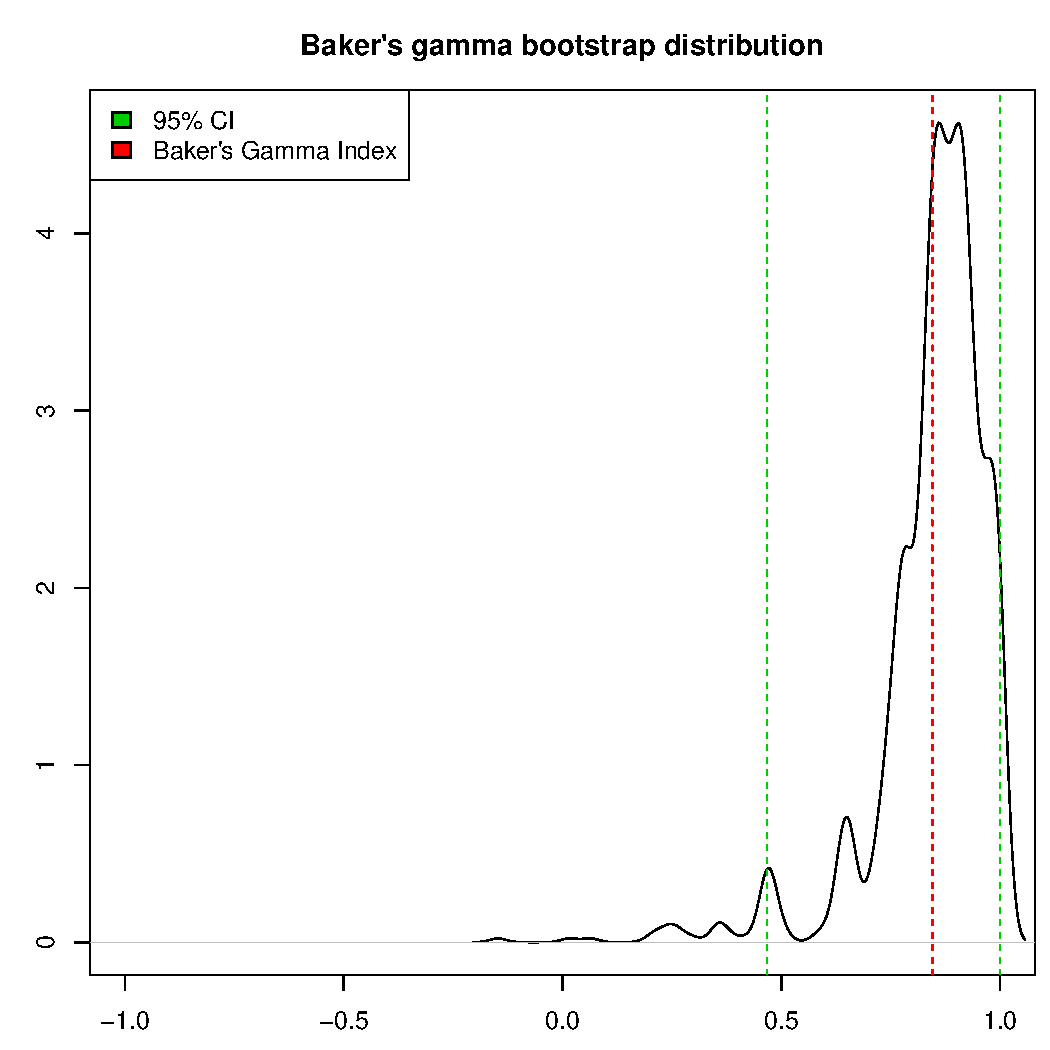
\includegraphics[width=\maxwidth]{figure/cor_bakers_gamma_simulation_CI_43} 

}



\end{knitrout}


We can see that in our case, the non-parametric bootstrap confidence-intervals reassures us that the correlation is significantly different than 0 (thank to the confidence-intervals duality with rejection regions). 




\subsection{Cophenetic correlation}

The cophenetic distance between two observations that have been clustered is defined to be the intergroup dissimilarity at which the two observations are first combined into a single cluster. This distance has many ties and restrictions. The cophenetic correlation \citep{sokal1962comparison} is the correlation between two cophenetic distance matrices of two trees.

The value can range between -1 to 1. With near 0 values meaning that the two trees are not statistically similar. For exact p-value one should result to a permutation test. One such option will be to permute over the labels of one tree many times, and calculating the distriubtion under the null hypothesis (keeping the trees topologies constant).

Here is a simple example:

\begin{knitrout}
\definecolor{shadecolor}{rgb}{0.969, 0.969, 0.969}\color{fgcolor}\begin{kframe}
\begin{alltt}
\hlkwd{set.seed}\hlstd{(}\hlnum{23235}\hlstd{)}
\hlstd{ss} \hlkwb{<-} \hlkwd{sample}\hlstd{(}\hlnum{1}\hlopt{:}\hlnum{150}\hlstd{,} \hlnum{10}\hlstd{)}
\hlstd{hc1} \hlkwb{<-} \hlkwd{hclust}\hlstd{(}\hlkwd{dist}\hlstd{(iris[ss,} \hlopt{-}\hlnum{5}\hlstd{]),} \hlstr{"com"}\hlstd{)}
\hlstd{hc2} \hlkwb{<-} \hlkwd{hclust}\hlstd{(}\hlkwd{dist}\hlstd{(iris[ss,} \hlopt{-}\hlnum{5}\hlstd{]),} \hlstr{"single"}\hlstd{)}
\hlstd{dend1} \hlkwb{<-} \hlkwd{as.dendrogram}\hlstd{(hc1)}
\hlstd{dend2} \hlkwb{<-} \hlkwd{as.dendrogram}\hlstd{(hc2)}
\hlcom{# cutree(dend1)}

\hlcom{# cophenetic(hc1) cophenetic(hc2) # notice how the dist}
\hlcom{# matrix for the dendrograms have different orders:}
\hlcom{# cophenetic(dend1) cophenetic(dend2)}

\hlkwd{cor}\hlstd{(}\hlkwd{cophenetic}\hlstd{(hc1),} \hlkwd{cophenetic}\hlstd{(hc2))}  \hlcom{# 0.874}
\end{alltt}
\begin{verbatim}
## [1] 0.4925
\end{verbatim}
\begin{alltt}
\hlkwd{cor}\hlstd{(}\hlkwd{cophenetic}\hlstd{(dend1),} \hlkwd{cophenetic}\hlstd{(dend2))}  \hlcom{# 0.16}
\end{alltt}
\begin{verbatim}
## [1] 0.3106
\end{verbatim}
\begin{alltt}
\hlcom{# the difference is becasue the order of the distance table}
\hlcom{# in the case of stats:::cophenetic.dendrogram will change}
\hlcom{# between dendrograms!}

\hlcom{# However, this is consistant (since I force-sort the}
\hlcom{# rows/columns):}
\hlkwd{cor_cophenetic}\hlstd{(hc1, hc2)}
\end{alltt}
\begin{verbatim}
## [1] 0.4925
\end{verbatim}
\begin{alltt}
\hlkwd{cor_cophenetic}\hlstd{(dend1, dend2)}
\end{alltt}
\begin{verbatim}
## [1] 0.4925
\end{verbatim}
\begin{alltt}
\hlcom{# we can also use different cor methods (almost the same}
\hlcom{# result though):}
\hlkwd{cor_cophenetic}\hlstd{(hc1, hc2,} \hlkwc{method} \hlstd{=} \hlstr{"spearman"}\hlstd{)}  \hlcom{# 0.8456014}
\end{alltt}
\begin{verbatim}
## [1] 0.5716
\end{verbatim}
\begin{alltt}
\hlkwd{cor_cophenetic}\hlstd{(dend1, dend2,} \hlkwc{method} \hlstd{=} \hlstr{"spearman"}\hlstd{)}  \hlcom{# }
\end{alltt}
\begin{verbatim}
## [1] 0.5716
\end{verbatim}
\begin{alltt}
\hlcom{# cophenetic correlation is about 10 times (!) faster than}
\hlcom{# bakers_gamma cor:}
\hlkwd{require}\hlstd{(microbenchmark)}
\hlkwd{microbenchmark}\hlstd{(}\hlkwc{cor_bakers_gamma} \hlstd{=} \hlkwd{cor_bakers_gamma}\hlstd{(dend1, dend2,}
    \hlkwc{try_cutree_hclust} \hlstd{=} \hlnum{FALSE}\hlstd{),} \hlkwc{cor_cophenetic} \hlstd{=} \hlkwd{cor_cophenetic}\hlstd{(dend1,}
    \hlstd{dend2),} \hlkwc{times} \hlstd{=} \hlnum{10}\hlstd{)}
\end{alltt}
\begin{verbatim}
## Unit: milliseconds
##              expr    min     lq median    uq    max neval
##  cor_bakers_gamma 100.15 100.88 102.04 107.3 113.22    10
##    cor_cophenetic  11.51  11.89  12.22  14.6  15.52    10
\end{verbatim}
\begin{alltt}
\hlcom{# but only because of the cutree for dendrogram. When}
\hlcom{# allowing hclust cutree it is only about twice as fast:}
\hlkwd{microbenchmark}\hlstd{(}\hlkwc{cor_bakers_gamma} \hlstd{=} \hlkwd{cor_bakers_gamma}\hlstd{(dend1, dend2,}
    \hlkwc{try_cutree_hclust} \hlstd{=} \hlnum{TRUE}\hlstd{),} \hlkwc{cor_cophenetic} \hlstd{=} \hlkwd{cor_cophenetic}\hlstd{(dend1,}
    \hlstd{dend2),} \hlkwc{times} \hlstd{=} \hlnum{10}\hlstd{)}
\end{alltt}
\begin{verbatim}
## Unit: milliseconds
##              expr   min    lq median    uq   max neval
##  cor_bakers_gamma 23.70 24.09  24.46 25.44 26.50    10
##    cor_cophenetic 11.38 11.80  12.35 14.61 18.61    10
\end{verbatim}
\end{kframe}
\end{knitrout}


An example of a permutation test:

\begin{knitrout}
\definecolor{shadecolor}{rgb}{0.969, 0.969, 0.969}\color{fgcolor}\begin{kframe}
\begin{alltt}
\hlkwd{set.seed}\hlstd{(}\hlnum{23235}\hlstd{)}
\hlstd{ss} \hlkwb{<-} \hlkwd{sample}\hlstd{(}\hlnum{1}\hlopt{:}\hlnum{150}\hlstd{,} \hlnum{10}\hlstd{)}  \hlcom{# we want to compare small trees}
\hlstd{hc1} \hlkwb{<-} \hlkwd{hclust}\hlstd{(}\hlkwd{dist}\hlstd{(iris[ss,} \hlopt{-}\hlnum{5}\hlstd{]),} \hlstr{"com"}\hlstd{)}
\hlstd{hc2} \hlkwb{<-} \hlkwd{hclust}\hlstd{(}\hlkwd{dist}\hlstd{(iris[ss,} \hlopt{-}\hlnum{5}\hlstd{]),} \hlstr{"single"}\hlstd{)}
\hlstd{dend1} \hlkwb{<-} \hlkwd{as.dendrogram}\hlstd{(hc1)}
\hlstd{dend2} \hlkwb{<-} \hlkwd{as.dendrogram}\hlstd{(hc2)}
\hlcom{# cutree(dend1)}

\hlstd{the_cor} \hlkwb{<-} \hlkwd{cor_cophenetic}\hlstd{(dend1, dend2)}
\hlstd{the_cor}
\end{alltt}
\begin{verbatim}
## [1] 0.4925
\end{verbatim}
\begin{alltt}
\hlstd{R} \hlkwb{<-} \hlnum{1000}
\hlstd{cor_cophenetic_results} \hlkwb{<-} \hlkwd{numeric}\hlstd{(R)}
\hlstd{dend_mixed1} \hlkwb{<-} \hlstd{dend1}
\hlstd{dend_mixed2} \hlkwb{<-} \hlstd{dend2}
\hlkwa{for} \hlstd{(i} \hlkwa{in} \hlnum{1}\hlopt{:}\hlstd{R) \{}
    \hlstd{dend_mixed1} \hlkwb{<-} \hlkwd{sample.dendrogram}\hlstd{(dend_mixed1,} \hlkwc{replace} \hlstd{=} \hlnum{FALSE}\hlstd{)}
    \hlstd{dend_mixed2} \hlkwb{<-} \hlkwd{sample.dendrogram}\hlstd{(dend_mixed2,} \hlkwc{replace} \hlstd{=} \hlnum{FALSE}\hlstd{)}
    \hlstd{cor_cophenetic_results[i]} \hlkwb{<-} \hlkwd{cor_cophenetic}\hlstd{(dend_mixed1,}
        \hlstd{dend_mixed2)}
\hlstd{\}}
\hlkwd{plot}\hlstd{(}\hlkwd{density}\hlstd{(cor_cophenetic_results),} \hlkwc{main} \hlstd{=} \hlstr{"Cophenetic correlation distribution under H0"}\hlstd{,}
    \hlkwc{xlim} \hlstd{=} \hlkwd{c}\hlstd{(}\hlopt{-}\hlnum{1}\hlstd{,} \hlnum{1}\hlstd{))}
\hlkwd{abline}\hlstd{(}\hlkwc{v} \hlstd{=} \hlnum{0}\hlstd{,} \hlkwc{lty} \hlstd{=} \hlnum{2}\hlstd{)}
\hlkwd{abline}\hlstd{(}\hlkwc{v} \hlstd{= the_cor,} \hlkwc{lty} \hlstd{=} \hlnum{2}\hlstd{,} \hlkwc{col} \hlstd{=} \hlnum{2}\hlstd{)}
\hlkwd{title}\hlstd{(}\hlkwc{sub} \hlstd{=} \hlkwd{paste}\hlstd{(}\hlstr{"One sided p-value ="}\hlstd{,} \hlkwd{round}\hlstd{(}\hlkwd{sum}\hlstd{(the_cor} \hlopt{<}
    \hlstd{cor_cophenetic_results)}\hlopt{/}\hlstd{R,} \hlnum{4}\hlstd{)))}
\end{alltt}
\end{kframe}

{\centering 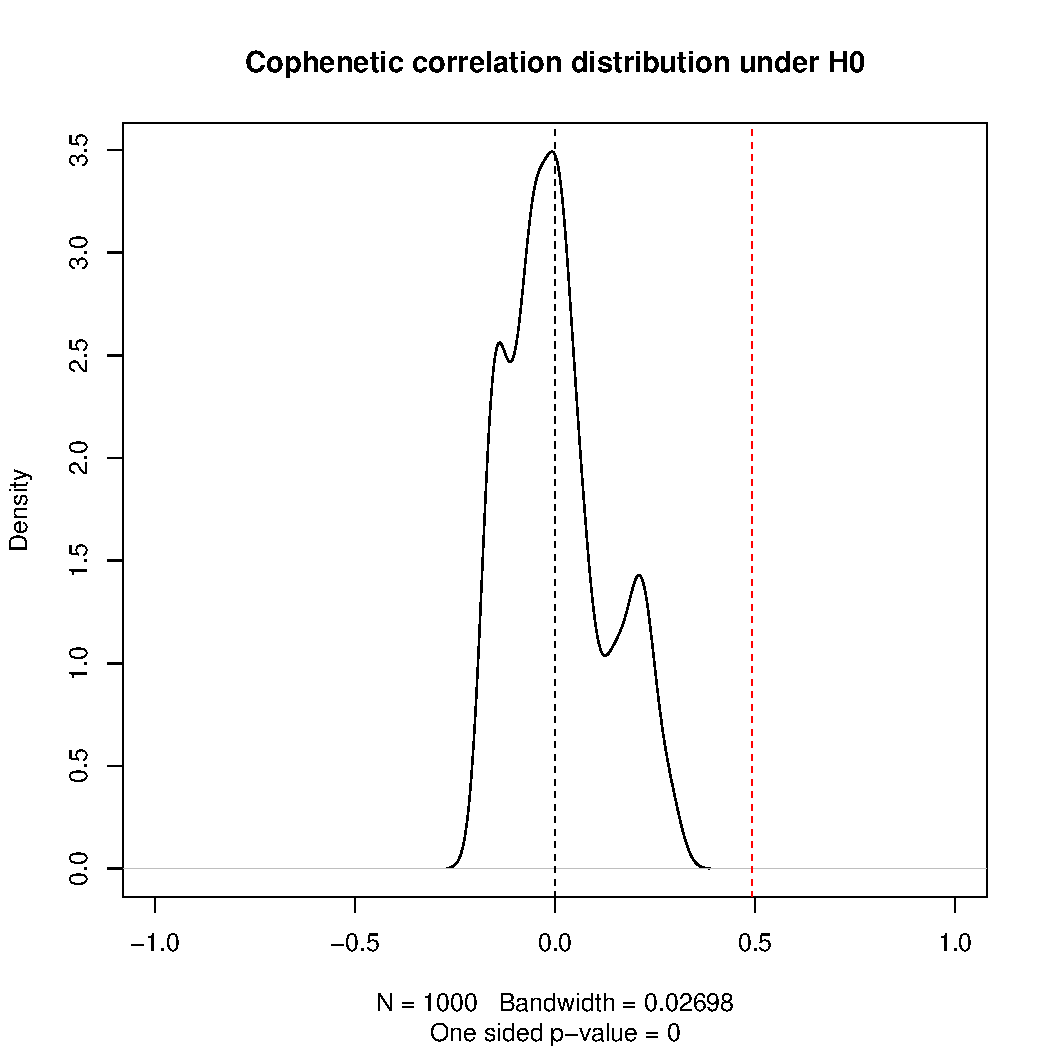
\includegraphics[width=\maxwidth]{figure/cor_cophenetic_simulation_2} 

}



\end{knitrout}




An example of a bootstrap CI (with method="pearson"):


\begin{knitrout}
\definecolor{shadecolor}{rgb}{0.969, 0.969, 0.969}\color{fgcolor}\begin{kframe}
\begin{alltt}
\hlkwd{set.seed}\hlstd{(}\hlnum{312356}\hlstd{)}
\hlstd{ss} \hlkwb{<-} \hlkwd{sample}\hlstd{(}\hlnum{1}\hlopt{:}\hlnum{150}\hlstd{,} \hlnum{10}\hlstd{)}  \hlcom{# we want to compare small trees}
\hlstd{hc1} \hlkwb{<-} \hlkwd{hclust}\hlstd{(}\hlkwd{dist}\hlstd{(iris[ss,} \hlopt{-}\hlnum{5}\hlstd{]),} \hlstr{"com"}\hlstd{)}
\hlstd{hc2} \hlkwb{<-} \hlkwd{hclust}\hlstd{(}\hlkwd{dist}\hlstd{(iris[ss,} \hlopt{-}\hlnum{5}\hlstd{]),} \hlstr{"single"}\hlstd{)}
\hlstd{dend1} \hlkwb{<-} \hlkwd{as.dendrogram}\hlstd{(hc1)}
\hlstd{dend2} \hlkwb{<-} \hlkwd{as.dendrogram}\hlstd{(hc2)}
\hlcom{# tanglegram(dend1, dend2) cutree(dend1)}

\hlstd{R} \hlkwb{<-} \hlnum{1000}
\hlstd{dend1_labels} \hlkwb{<-} \hlkwd{labels}\hlstd{(dend1)}
\hlstd{dend2_labels} \hlkwb{<-} \hlkwd{labels}\hlstd{(dend2)}
\hlstd{cor_cophenetic_results} \hlkwb{<-} \hlkwd{numeric}\hlstd{(R)}
\hlkwa{for} \hlstd{(i} \hlkwa{in} \hlnum{1}\hlopt{:}\hlstd{R) \{}
    \hlstd{sampled_labels} \hlkwb{<-} \hlkwd{sample}\hlstd{(dend1_labels,} \hlkwc{replace} \hlstd{=} \hlnum{TRUE}\hlstd{)}
    \hlcom{# members needs to be fixed since it will be later used in}
    \hlcom{# nleaves}
    \hlstd{dend_mixed1} \hlkwb{<-} \hlkwd{sample.dendrogram}\hlstd{(dend1,} \hlkwc{dend_labels} \hlstd{= dend1_labels,}
        \hlkwc{fix_members} \hlstd{=} \hlnum{TRUE}\hlstd{,} \hlkwc{fix_order} \hlstd{=} \hlnum{TRUE}\hlstd{,} \hlkwc{fix_midpoint} \hlstd{=} \hlnum{FALSE}\hlstd{,}
        \hlkwc{replace} \hlstd{=} \hlnum{TRUE}\hlstd{,} \hlkwc{sampled_labels} \hlstd{= sampled_labels)}
    \hlstd{dend_mixed2} \hlkwb{<-} \hlkwd{sample.dendrogram}\hlstd{(dend2,} \hlkwc{dend_labels} \hlstd{= dend2_labels,}
        \hlkwc{fix_members} \hlstd{=} \hlnum{TRUE}\hlstd{,} \hlkwc{fix_order} \hlstd{=} \hlnum{TRUE}\hlstd{,} \hlkwc{fix_midpoint} \hlstd{=} \hlnum{FALSE}\hlstd{,}
        \hlkwc{replace} \hlstd{=} \hlnum{TRUE}\hlstd{,} \hlkwc{sampled_labels} \hlstd{= sampled_labels)}
    \hlstd{cor_cophenetic_results[i]} \hlkwb{<-} \hlkwd{cor_cophenetic}\hlstd{(dend_mixed1,}
        \hlstd{dend_mixed2,} \hlkwc{warn} \hlstd{=} \hlnum{FALSE}\hlstd{)}
\hlstd{\}}


\hlcom{# here is the tanglegram tanglegram(dend1, dend2) And here is}
\hlcom{# the tanglegram for one sample of our trees:}
\hlstd{dend_mixed1} \hlkwb{<-} \hlkwd{rank_order.dendrogram}\hlstd{(dend_mixed1)}
\hlstd{dend_mixed2} \hlkwb{<-} \hlkwd{rank_order.dendrogram}\hlstd{(dend_mixed2)}
\hlstd{dend_mixed1} \hlkwb{<-} \hlkwd{fix_members_attr.dendrogram}\hlstd{(dend_mixed1)}
\hlstd{dend_mixed2} \hlkwb{<-} \hlkwd{fix_members_attr.dendrogram}\hlstd{(dend_mixed2)}
\hlcom{# tanglegram(dend_mixed1, dend_mixed2)}
\hlkwd{cor_cophenetic}\hlstd{(dend_mixed1, dend_mixed2,} \hlkwc{warn} \hlstd{=} \hlnum{FALSE}\hlstd{)}
\end{alltt}
\begin{verbatim}
## [1] 0.9981
\end{verbatim}
\begin{alltt}
\hlstd{CI95} \hlkwb{<-} \hlkwd{quantile}\hlstd{(cor_cophenetic_results,} \hlkwc{probs} \hlstd{=} \hlkwd{c}\hlstd{(}\hlnum{0.025}\hlstd{,} \hlnum{0.975}\hlstd{))}
\hlstd{CI95}
\end{alltt}
\begin{verbatim}
##   2.5%  97.5% 
## 0.5253 0.9943
\end{verbatim}
\begin{alltt}
\hlkwd{par}\hlstd{(}\hlkwc{mfrow} \hlstd{=} \hlkwd{c}\hlstd{(}\hlnum{1}\hlstd{,} \hlnum{1}\hlstd{))}
\hlkwd{plot}\hlstd{(}\hlkwd{density}\hlstd{(cor_cophenetic_results),} \hlkwc{main} \hlstd{=} \hlstr{"Cophenetic correlation - bootstrap distribution"}\hlstd{,}
    \hlkwc{xlim} \hlstd{=} \hlkwd{c}\hlstd{(}\hlopt{-}\hlnum{1}\hlstd{,} \hlnum{1}\hlstd{))}
\hlkwd{abline}\hlstd{(}\hlkwc{v} \hlstd{= CI95,} \hlkwc{lty} \hlstd{=} \hlnum{2}\hlstd{,} \hlkwc{col} \hlstd{=} \hlnum{3}\hlstd{)}
\hlkwd{abline}\hlstd{(}\hlkwc{v} \hlstd{=} \hlkwd{cor_cophenetic}\hlstd{(dend1, dend2),} \hlkwc{lty} \hlstd{=} \hlnum{2}\hlstd{,} \hlkwc{col} \hlstd{=} \hlnum{2}\hlstd{)}
\hlkwd{legend}\hlstd{(}\hlstr{"topleft"}\hlstd{,} \hlkwc{legend} \hlstd{=} \hlkwd{c}\hlstd{(}\hlstr{"95% CI"}\hlstd{,} \hlstr{"Cophenetic correlation"}\hlstd{),}
    \hlkwc{fill} \hlstd{=} \hlkwd{c}\hlstd{(}\hlnum{3}\hlstd{,} \hlnum{2}\hlstd{))}
\end{alltt}
\end{kframe}

{\centering 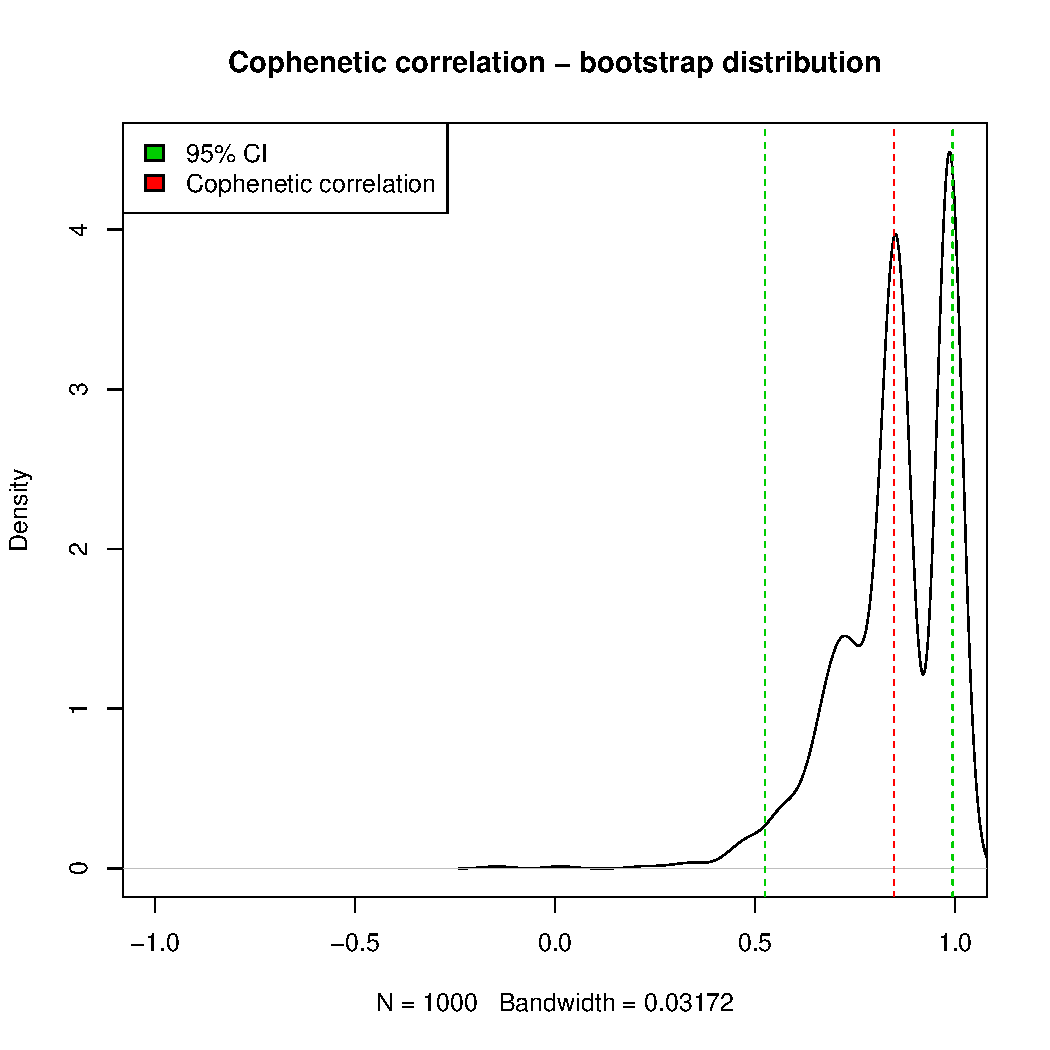
\includegraphics[width=\maxwidth]{figure/cor_cophenetic_simulation_CI_3} 

}



\end{knitrout}



An example of a bootstrap CI (with method="spearman"):


\begin{knitrout}
\definecolor{shadecolor}{rgb}{0.969, 0.969, 0.969}\color{fgcolor}\begin{kframe}
\begin{alltt}
\hlkwd{set.seed}\hlstd{(}\hlnum{312356}\hlstd{)}
\hlstd{ss} \hlkwb{<-} \hlkwd{sample}\hlstd{(}\hlnum{1}\hlopt{:}\hlnum{150}\hlstd{,} \hlnum{10}\hlstd{)}  \hlcom{# we want to compare small trees}
\hlstd{hc1} \hlkwb{<-} \hlkwd{hclust}\hlstd{(}\hlkwd{dist}\hlstd{(iris[ss,} \hlopt{-}\hlnum{5}\hlstd{]),} \hlstr{"com"}\hlstd{)}
\hlstd{hc2} \hlkwb{<-} \hlkwd{hclust}\hlstd{(}\hlkwd{dist}\hlstd{(iris[ss,} \hlopt{-}\hlnum{5}\hlstd{]),} \hlstr{"single"}\hlstd{)}
\hlstd{dend1} \hlkwb{<-} \hlkwd{as.dendrogram}\hlstd{(hc1)}
\hlstd{dend2} \hlkwb{<-} \hlkwd{as.dendrogram}\hlstd{(hc2)}
\hlcom{# tanglegram(dend1, dend2) cutree(dend1)}

\hlstd{R} \hlkwb{<-} \hlnum{1000}
\hlstd{dend1_labels} \hlkwb{<-} \hlkwd{labels}\hlstd{(dend1)}
\hlstd{dend2_labels} \hlkwb{<-} \hlkwd{labels}\hlstd{(dend2)}
\hlstd{cor_cophenetic_results} \hlkwb{<-} \hlkwd{numeric}\hlstd{(R)}
\hlkwa{for} \hlstd{(i} \hlkwa{in} \hlnum{1}\hlopt{:}\hlstd{R) \{}
    \hlstd{sampled_labels} \hlkwb{<-} \hlkwd{sample}\hlstd{(dend1_labels,} \hlkwc{replace} \hlstd{=} \hlnum{TRUE}\hlstd{)}
    \hlcom{# members needs to be fixed since it will be later used in}
    \hlcom{# nleaves}
    \hlstd{dend_mixed1} \hlkwb{<-} \hlkwd{sample.dendrogram}\hlstd{(dend1,} \hlkwc{dend_labels} \hlstd{= dend1_labels,}
        \hlkwc{fix_members} \hlstd{=} \hlnum{TRUE}\hlstd{,} \hlkwc{fix_order} \hlstd{=} \hlnum{TRUE}\hlstd{,} \hlkwc{fix_midpoint} \hlstd{=} \hlnum{FALSE}\hlstd{,}
        \hlkwc{replace} \hlstd{=} \hlnum{TRUE}\hlstd{,} \hlkwc{sampled_labels} \hlstd{= sampled_labels)}
    \hlstd{dend_mixed2} \hlkwb{<-} \hlkwd{sample.dendrogram}\hlstd{(dend2,} \hlkwc{dend_labels} \hlstd{= dend2_labels,}
        \hlkwc{fix_members} \hlstd{=} \hlnum{TRUE}\hlstd{,} \hlkwc{fix_order} \hlstd{=} \hlnum{TRUE}\hlstd{,} \hlkwc{fix_midpoint} \hlstd{=} \hlnum{FALSE}\hlstd{,}
        \hlkwc{replace} \hlstd{=} \hlnum{TRUE}\hlstd{,} \hlkwc{sampled_labels} \hlstd{= sampled_labels)}
    \hlstd{cor_cophenetic_results[i]} \hlkwb{<-} \hlkwd{cor_cophenetic}\hlstd{(dend_mixed1,}
        \hlstd{dend_mixed2,} \hlkwc{warn} \hlstd{=} \hlnum{FALSE}\hlstd{,} \hlkwc{method} \hlstd{=} \hlstr{"spearman"}\hlstd{)}
\hlstd{\}}


\hlcom{# here is the tanglegram tanglegram(dend1, dend2) And here is}
\hlcom{# the tanglegram for one sample of our trees:}
\hlstd{dend_mixed1} \hlkwb{<-} \hlkwd{rank_order.dendrogram}\hlstd{(dend_mixed1)}
\hlstd{dend_mixed2} \hlkwb{<-} \hlkwd{rank_order.dendrogram}\hlstd{(dend_mixed2)}
\hlstd{dend_mixed1} \hlkwb{<-} \hlkwd{fix_members_attr.dendrogram}\hlstd{(dend_mixed1)}
\hlstd{dend_mixed2} \hlkwb{<-} \hlkwd{fix_members_attr.dendrogram}\hlstd{(dend_mixed2)}
\hlcom{# tanglegram(dend_mixed1, dend_mixed2)}
\hlkwd{cor_cophenetic}\hlstd{(dend_mixed1, dend_mixed2,} \hlkwc{warn} \hlstd{=} \hlnum{FALSE}\hlstd{,} \hlkwc{method} \hlstd{=} \hlstr{"spearman"}\hlstd{)}
\end{alltt}
\begin{verbatim}
## [1] 0.9924
\end{verbatim}
\begin{alltt}
\hlstd{CI95} \hlkwb{<-} \hlkwd{quantile}\hlstd{(cor_cophenetic_results,} \hlkwc{probs} \hlstd{=} \hlkwd{c}\hlstd{(}\hlnum{0.025}\hlstd{,} \hlnum{0.975}\hlstd{))}
\hlstd{CI95}
\end{alltt}
\begin{verbatim}
##   2.5%  97.5% 
## 0.4753 1.0000
\end{verbatim}
\begin{alltt}
\hlkwd{par}\hlstd{(}\hlkwc{mfrow} \hlstd{=} \hlkwd{c}\hlstd{(}\hlnum{1}\hlstd{,} \hlnum{1}\hlstd{))}
\hlkwd{plot}\hlstd{(}\hlkwd{density}\hlstd{(cor_cophenetic_results),} \hlkwc{main} \hlstd{=} \hlstr{"Cophenetic correlation - bootstrap distribution"}\hlstd{,}
    \hlkwc{xlim} \hlstd{=} \hlkwd{c}\hlstd{(}\hlopt{-}\hlnum{1}\hlstd{,} \hlnum{1}\hlstd{))}
\hlkwd{abline}\hlstd{(}\hlkwc{v} \hlstd{= CI95,} \hlkwc{lty} \hlstd{=} \hlnum{2}\hlstd{,} \hlkwc{col} \hlstd{=} \hlnum{3}\hlstd{)}
\hlkwd{abline}\hlstd{(}\hlkwc{v} \hlstd{=} \hlkwd{cor_cophenetic}\hlstd{(dend1, dend2,} \hlkwc{method} \hlstd{=} \hlstr{"spearman"}\hlstd{),}
    \hlkwc{lty} \hlstd{=} \hlnum{2}\hlstd{,} \hlkwc{col} \hlstd{=} \hlnum{2}\hlstd{)}
\hlkwd{legend}\hlstd{(}\hlstr{"topleft"}\hlstd{,} \hlkwc{legend} \hlstd{=} \hlkwd{c}\hlstd{(}\hlstr{"95% CI"}\hlstd{,} \hlstr{"Cophenetic correlation"}\hlstd{),}
    \hlkwc{fill} \hlstd{=} \hlkwd{c}\hlstd{(}\hlnum{3}\hlstd{,} \hlnum{2}\hlstd{))}
\end{alltt}
\end{kframe}

{\centering 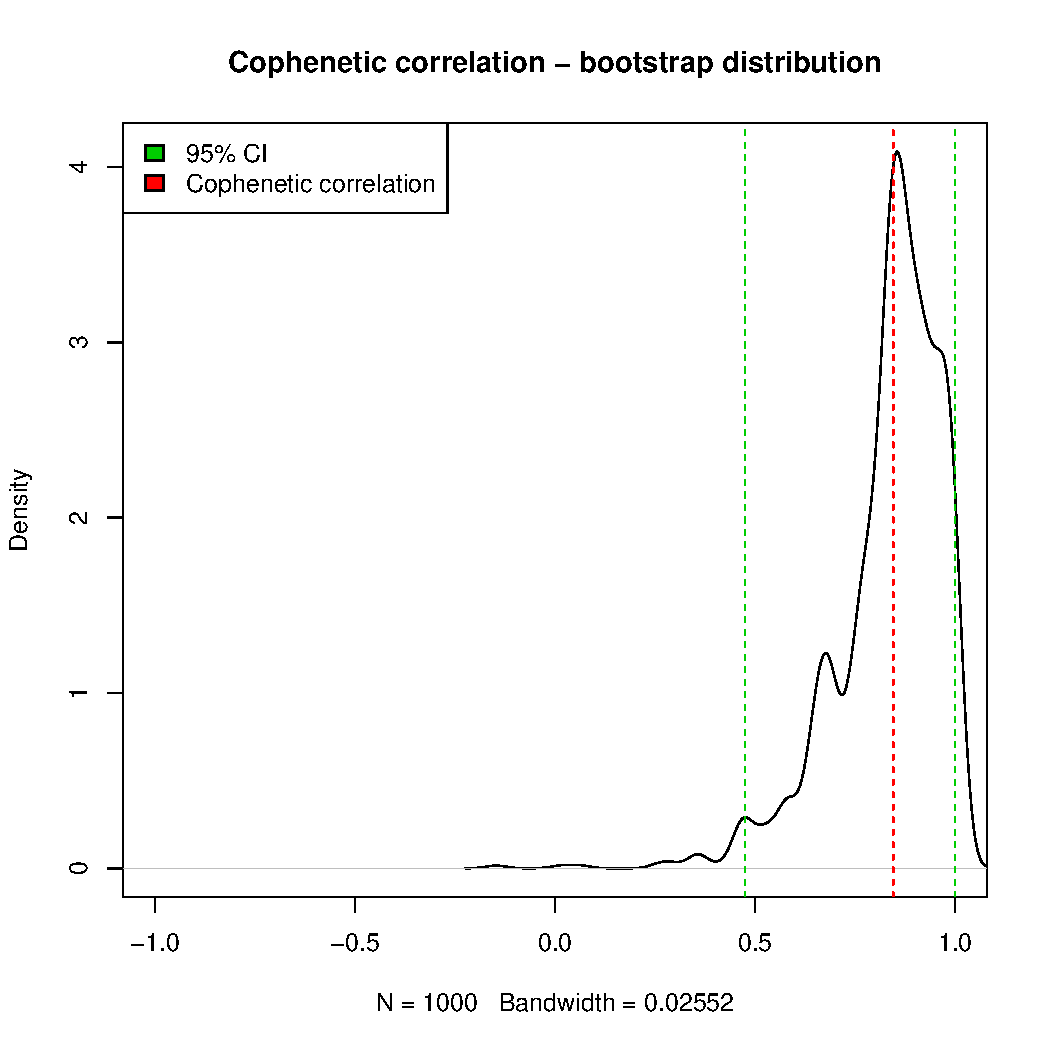
\includegraphics[width=\maxwidth]{figure/cor_cophenetic_simulation_CI_4} 

}



\end{knitrout}





\subsection{The Fowlkes-Mallows Index and the Bk plot}

\subsubsection{The Fowlkes-Mallows Index}

The Fowlkes-Mallows Index \citep{fowlkes1983method} (FM Index, or Bk) is a measure of similarity between two clusterings. The FM index ranges from 0 to 1, a higher value indicates a greater similarity between the two clusters.

The \pkg{dendextend} package allows the calculation of FM-Index, its expectancy and variance under the null hypothesis, and a creation of permutations of the FM-Index under $H_0$. Thanks to the \pkg{profdpm} package \citep{CRAN:profdpm}, we have another example of calculating the FM (though it does not offer the expectancy and variance under $H_0$):

\begin{knitrout}
\definecolor{shadecolor}{rgb}{0.969, 0.969, 0.969}\color{fgcolor}\begin{kframe}
\begin{alltt}
\hlstd{ss} \hlkwb{<-} \hlnum{TRUE}  \hlcom{# sample(1:150, 10 )}
\hlstd{hc1} \hlkwb{<-} \hlkwd{hclust}\hlstd{(}\hlkwd{dist}\hlstd{(iris[ss,} \hlopt{-}\hlnum{5}\hlstd{]),} \hlstr{"com"}\hlstd{)}
\hlstd{hc2} \hlkwb{<-} \hlkwd{hclust}\hlstd{(}\hlkwd{dist}\hlstd{(iris[ss,} \hlopt{-}\hlnum{5}\hlstd{]),} \hlstr{"single"}\hlstd{)}

\hlcom{# FM index of a cluster with himself is 1:}
\hlkwd{FM_index}\hlstd{(}\hlkwd{cutree}\hlstd{(hc1,} \hlkwc{k} \hlstd{=} \hlnum{3}\hlstd{),} \hlkwd{cutree}\hlstd{(hc1,} \hlkwc{k} \hlstd{=} \hlnum{3}\hlstd{))}
\end{alltt}
\begin{verbatim}
## [1] 1
## attr(,"E_FM")
## [1] 0.3722
## attr(,"V_FM")
## [1] 5.985e-05
\end{verbatim}
\begin{alltt}
\hlcom{# FM index of two clusterings:}
\hlkwd{FM_index}\hlstd{(}\hlkwd{cutree}\hlstd{(hc1,} \hlkwc{k} \hlstd{=} \hlnum{3}\hlstd{),} \hlkwd{cutree}\hlstd{(hc2,} \hlkwc{k} \hlstd{=} \hlnum{3}\hlstd{))}
\end{alltt}
\begin{verbatim}
## [1] 0.806
## attr(,"E_FM")
## [1] 0.4462
## attr(,"V_FM")
## [1] 6.464e-05
\end{verbatim}
\begin{alltt}
\hlcom{# we got a value far above the expected under H0}

\hlcom{# Using the R code:}
\hlkwd{FM_index_R}\hlstd{(}\hlkwd{cutree}\hlstd{(hc1,} \hlkwc{k} \hlstd{=} \hlnum{3}\hlstd{),} \hlkwd{cutree}\hlstd{(hc2,} \hlkwc{k} \hlstd{=} \hlnum{3}\hlstd{))}
\end{alltt}
\begin{verbatim}
## [1] 0.806
## attr(,"E_FM")
## [1] 0.4462
## attr(,"V_FM")
## [1] 6.464e-05
\end{verbatim}
\begin{alltt}
\hlcom{# Or wrapping the code from profdpm: (notice the NA's)}
\hlkwd{FM_index_profdpm}\hlstd{(}\hlkwd{cutree}\hlstd{(hc1,} \hlkwc{k} \hlstd{=} \hlnum{3}\hlstd{),} \hlkwd{cutree}\hlstd{(hc2,} \hlkwc{k} \hlstd{=} \hlnum{3}\hlstd{))}
\end{alltt}
\begin{verbatim}
## [1] 0.806
## attr(,"E_FM")
## [1] NA
## attr(,"V_FM")
## [1] NA
\end{verbatim}
\begin{alltt}


\end{alltt}
\end{kframe}
\end{knitrout}


The distribution of FM is interesting for medium sized k (25), we can test it using a permutation test:

\begin{knitrout}
\definecolor{shadecolor}{rgb}{0.969, 0.969, 0.969}\color{fgcolor}\begin{kframe}
\begin{alltt}
\hlkwd{set.seed}\hlstd{(}\hlnum{23235}\hlstd{)}
\hlstd{ss} \hlkwb{<-} \hlnum{TRUE}  \hlcom{# sample(1:150, 10 )}
\hlstd{hc1} \hlkwb{<-} \hlkwd{hclust}\hlstd{(}\hlkwd{dist}\hlstd{(iris[ss,} \hlopt{-}\hlnum{5}\hlstd{]),} \hlstr{"com"}\hlstd{)}
\hlstd{hc2} \hlkwb{<-} \hlkwd{hclust}\hlstd{(}\hlkwd{dist}\hlstd{(iris[ss,} \hlopt{-}\hlnum{5}\hlstd{]),} \hlstr{"single"}\hlstd{)}
\hlcom{# dend1 <- as.dendrogram(hc1) dend2 <- as.dendrogram(hc2)}
\hlcom{# cutree(dend1)}

\hlcom{# # small k A1_clusters <- cutree(hc1, k=3) # will give a}
\hlcom{# right tailed distribution # large k A1_clusters <-}
\hlcom{# cutree(hc1, k=50) # will give a discrete distribution}
\hlcom{# 'medium' k}
\hlstd{A1_clusters} \hlkwb{<-} \hlkwd{cutree}\hlstd{(hc1,} \hlkwc{k} \hlstd{=} \hlnum{25}\hlstd{)}  \hlcom{# gives almost the normal distribution!}
\hlstd{A2_clusters} \hlkwb{<-} \hlstd{A1_clusters}

\hlstd{R} \hlkwb{<-} \hlnum{10000}
\hlkwd{set.seed}\hlstd{(}\hlnum{414130}\hlstd{)}
\hlstd{FM_index_H0} \hlkwb{<-} \hlkwd{replicate}\hlstd{(R,} \hlkwd{FM_index_permutation}\hlstd{(A1_clusters,}
    \hlstd{A2_clusters))}  \hlcom{# can take 10 sec}
\hlkwd{plot}\hlstd{(}\hlkwd{density}\hlstd{(FM_index_H0),} \hlkwc{main} \hlstd{=} \hlstr{"FM Index distribution under H0\textbackslash{}n (10000 permutation)"}\hlstd{)}
\hlkwd{abline}\hlstd{(}\hlkwc{v} \hlstd{=} \hlkwd{mean}\hlstd{(FM_index_H0),} \hlkwc{col} \hlstd{=} \hlnum{1}\hlstd{,} \hlkwc{lty} \hlstd{=} \hlnum{2}\hlstd{)}
\hlcom{# The permutation distribution is with a heavy right tail:}
\hlcom{# require(psych) skew(FM_index_H0) # 1.254}
\hlcom{# kurtosi(FM_index_H0) # 2.5427}

\hlkwd{mean}\hlstd{(FM_index_H0)}
\end{alltt}
\begin{verbatim}
## [1] 0.05151
\end{verbatim}
\begin{alltt}
\hlkwd{var}\hlstd{(FM_index_H0)}
\end{alltt}
\begin{verbatim}
## [1] 8.28e-05
\end{verbatim}
\begin{alltt}
\hlstd{the_FM_index} \hlkwb{<-} \hlkwd{FM_index}\hlstd{(A1_clusters, A2_clusters)}
\hlstd{the_FM_index}
\end{alltt}
\begin{verbatim}
## [1] 1
## attr(,"E_FM")
## [1] 0.05154
## attr(,"V_FM")
## [1] 8.415e-05
\end{verbatim}
\begin{alltt}
\hlstd{our_dnorm} \hlkwb{<-} \hlkwa{function}\hlstd{(}\hlkwc{x}\hlstd{) \{}
    \hlkwd{dnorm}\hlstd{(x,} \hlkwc{mean} \hlstd{=} \hlkwd{attr}\hlstd{(the_FM_index,} \hlstr{"E_FM"}\hlstd{),} \hlkwc{sd} \hlstd{=} \hlkwd{sqrt}\hlstd{(}\hlkwd{attr}\hlstd{(the_FM_index,}
        \hlstr{"V_FM"}\hlstd{)))}
\hlstd{\}}
\hlcom{# our_dnorm(0.35)}
\hlkwd{curve}\hlstd{(our_dnorm,} \hlkwc{col} \hlstd{=} \hlnum{4}\hlstd{,} \hlkwc{from} \hlstd{=} \hlopt{-}\hlnum{1}\hlstd{,} \hlkwc{to} \hlstd{=} \hlnum{1}\hlstd{,} \hlkwc{n} \hlstd{= R,} \hlkwc{add} \hlstd{=} \hlnum{TRUE}\hlstd{)}
\hlkwd{abline}\hlstd{(}\hlkwc{v} \hlstd{=} \hlkwd{attr}\hlstd{(the_FM_index,} \hlstr{"E_FM"}\hlstd{),} \hlkwc{col} \hlstd{=} \hlnum{4}\hlstd{,} \hlkwc{lty} \hlstd{=} \hlnum{2}\hlstd{)}

\hlkwd{legend}\hlstd{(}\hlstr{"topright"}\hlstd{,} \hlkwc{legend} \hlstd{=} \hlkwd{c}\hlstd{(}\hlstr{"asymptotic"}\hlstd{,} \hlstr{"permutation"}\hlstd{),} \hlkwc{fill} \hlstd{=} \hlkwd{c}\hlstd{(}\hlnum{4}\hlstd{,}
    \hlnum{1}\hlstd{))}
\end{alltt}
\end{kframe}

{\centering 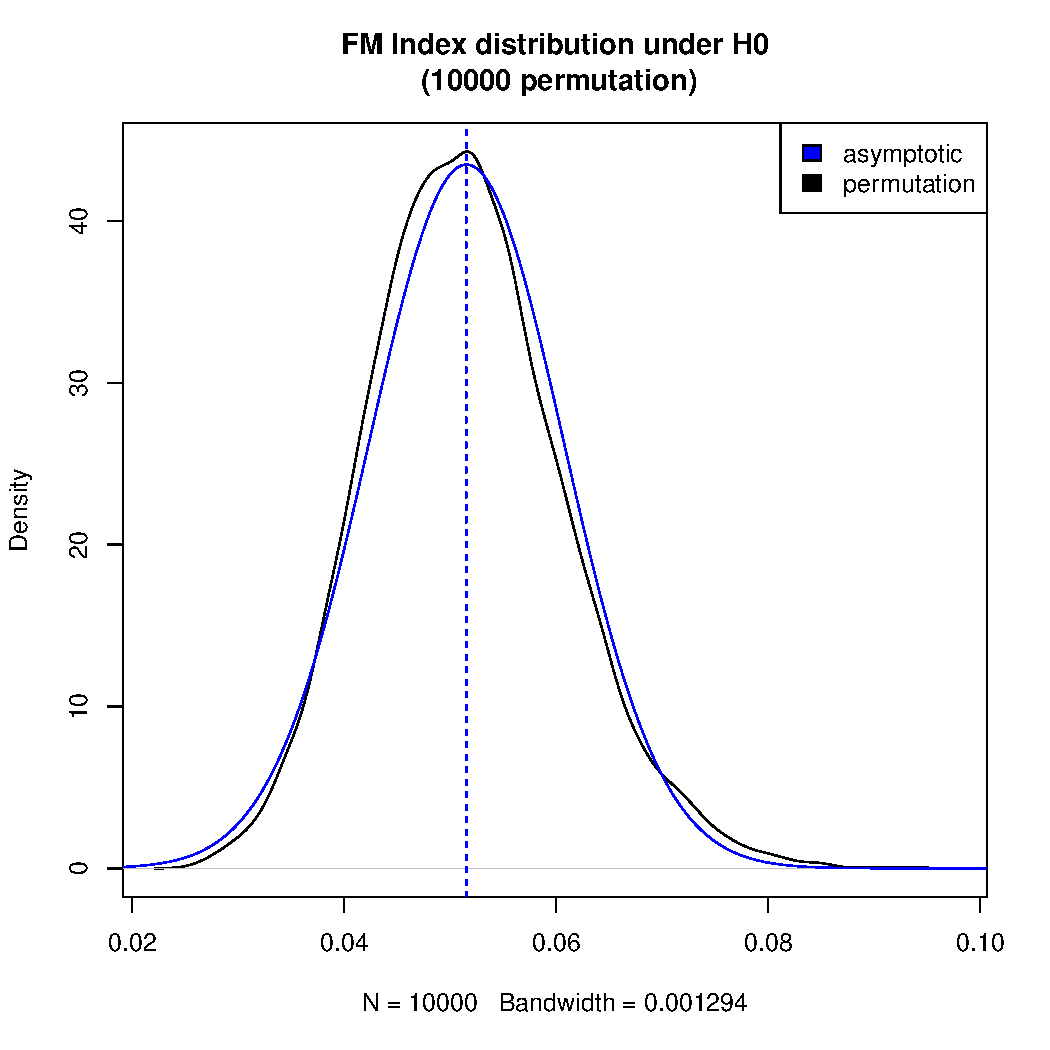
\includegraphics[width=\maxwidth]{figure/FM_permutation_example_1} 

}



\end{knitrout}


It is interesting to compare how the two ditributions diverge when K (3) is smaller:


\begin{knitrout}
\definecolor{shadecolor}{rgb}{0.969, 0.969, 0.969}\color{fgcolor}\begin{kframe}
\begin{verbatim}
## [1] 5.923e-05
## [1] 1
## attr(,"E_FM")
## [1] 0.3722
## attr(,"V_FM")
## [1] 5.985e-05
\end{verbatim}
\end{kframe}

{\centering 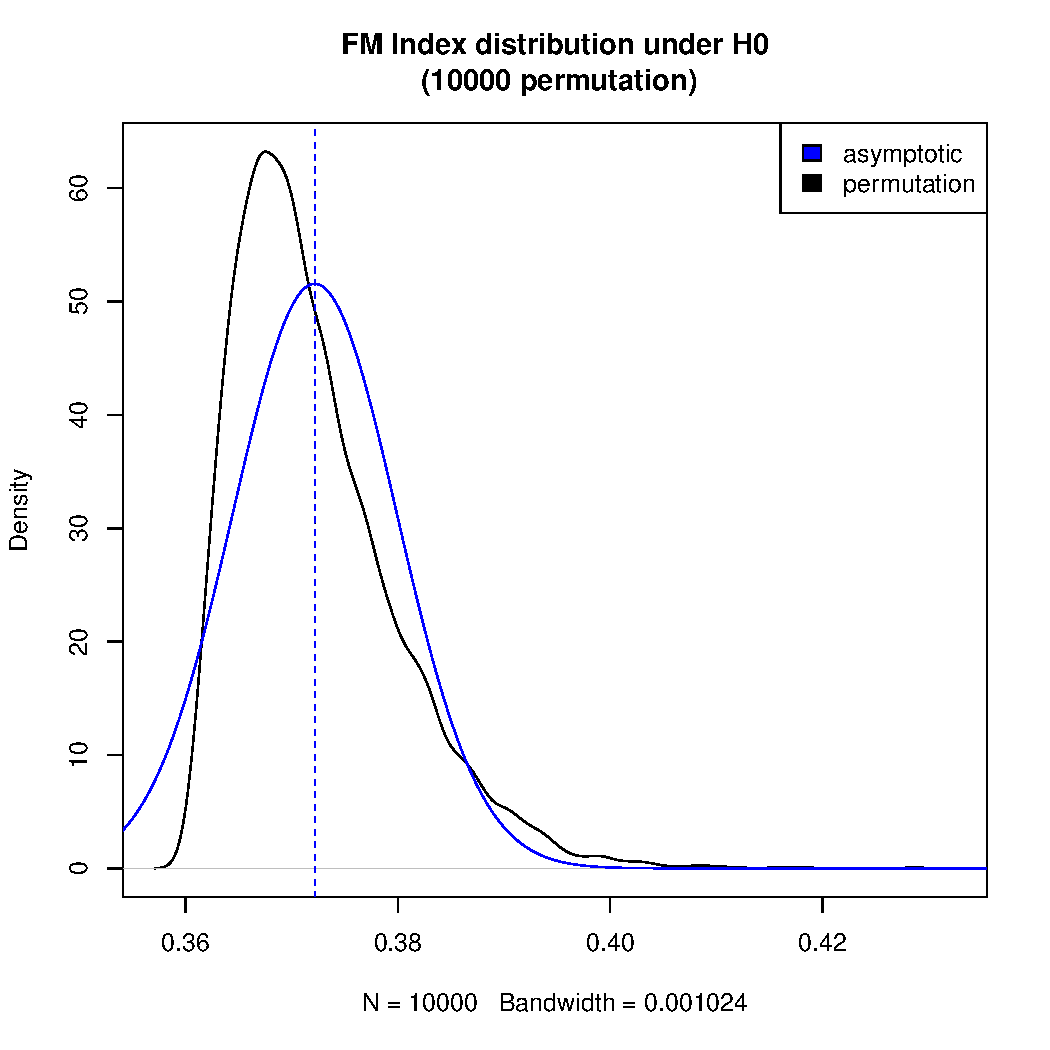
\includegraphics[width=\maxwidth]{figure/FM_permutation_example_2} 

}



\end{knitrout}


Or of how it will look when K (80) is large (and the distribution becomes discrete):


\begin{knitrout}
\definecolor{shadecolor}{rgb}{0.969, 0.969, 0.969}\color{fgcolor}\begin{kframe}
\begin{verbatim}
## [1] 8.89e-05
## [1] 1
## attr(,"E_FM")
## [1] 0.01136
## attr(,"V_FM")
## [1] 8.86e-05
\end{verbatim}
\end{kframe}

{\centering 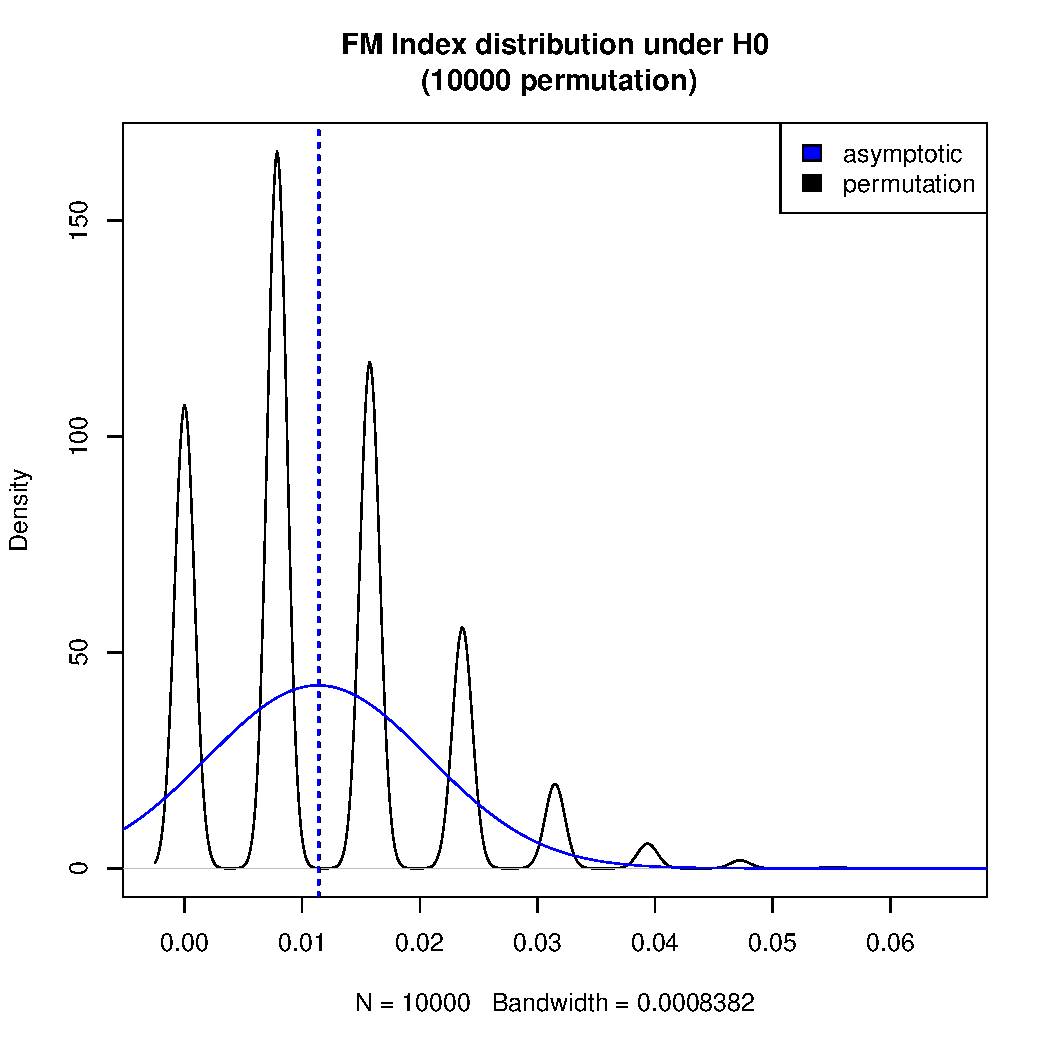
\includegraphics[width=\maxwidth]{figure/FM_permutation_example_3} 

}



\end{knitrout}


\subsubsection{The Bk plot}


In the Bk method we calculate the FM Index (Bk) for each k (k=2,3,…,n-1) number of clusters, giving the association between the two trees when each is cut to have k groups. The similarity between two hierarchical clustering dendrograms, can be investigated, using the (k,Bk) plot: For every level of splitting of the two dendrograms which produces k clusters in each tree, the plot shows the number Bk, and therefore enables the investigation of potential nuances in the structure of similarity. The Bk measures the number of pairs of items which are in the same cluster in both dendrograms, one of the clusters in one of the trees and one of the clusters in the other tree, divided by the geometric mean of the number of pairs of items which are in the same cluster in each tree. Namely, ${a_{uv}} = 1\left( {or{\rm{ }}{{\rm{b}}_{uv}} = 1} \right)$ if the items u and v are in the same cluster in the first tree (second tree), when it is cut so to give k clusters, and otherwise 0:

\[{FM_k} = {B_k} = \frac{{\sum\limits_{}^{} {{a_{uv}}{b_{uv}}} }}{{\sqrt {\sum\limits_{}^{} {{a_{uv}}} \sum\limits_{}^{} {{b_{uv}}} } }}\]

The Bk measure can be plotted for every value of k (except k=n) in order to create the “(k,Bk) plot”.  The plot compares the similarity of the two trees for different cuts. The mean and variance of Bk, under the null hypothesis (that the two trees are not “similar”), and under the assumption that the margins of the matching matrix are fixed, are given in Fowlkes and Mallows \citep{fowlkes1983method}. They allow making inference on whether the results obtained are different from what would have been expected under the null hypothesis (of now particular order of the trees' labels).

The \code{Bk} and the \code{Bk_plot} functions allow the calculation of the FM-Index for a range of k values on two trees. Here are examples:

\begin{knitrout}
\definecolor{shadecolor}{rgb}{0.969, 0.969, 0.969}\color{fgcolor}\begin{kframe}
\begin{alltt}
\hlkwd{set.seed}\hlstd{(}\hlnum{23235}\hlstd{)}
\hlstd{ss} \hlkwb{<-} \hlnum{TRUE}  \hlcom{# sample(1:150, 30 ) # TRUE #}
\hlstd{hc1} \hlkwb{<-} \hlkwd{hclust}\hlstd{(}\hlkwd{dist}\hlstd{(iris[ss,} \hlopt{-}\hlnum{5}\hlstd{]),} \hlstr{"com"}\hlstd{)}
\hlstd{hc2} \hlkwb{<-} \hlkwd{hclust}\hlstd{(}\hlkwd{dist}\hlstd{(iris[ss,} \hlopt{-}\hlnum{5}\hlstd{]),} \hlstr{"single"}\hlstd{)}
\hlstd{dend1} \hlkwb{<-} \hlkwd{as.dendrogram}\hlstd{(hc1)}
\hlstd{dend2} \hlkwb{<-} \hlkwd{as.dendrogram}\hlstd{(hc2)}
\hlcom{# cutree(tree1)}

\hlcom{# It works the same for hclust and dendrograms:}
\hlkwd{Bk}\hlstd{(hc1, hc2,} \hlkwc{k} \hlstd{=} \hlnum{3}\hlstd{)}
\end{alltt}
\begin{verbatim}
## $`3`
## [1] 0.806
## attr(,"E_FM")
## [1] 0.4462
## attr(,"V_FM")
## [1] 6.464e-05
\end{verbatim}
\begin{alltt}
\hlkwd{Bk}\hlstd{(dend1, dend2,} \hlkwc{k} \hlstd{=} \hlnum{3}\hlstd{)}
\end{alltt}
\begin{verbatim}
## $`3`
## [1] 0.806
## attr(,"E_FM")
## [1] 0.4462
## attr(,"V_FM")
## [1] 6.464e-05
\end{verbatim}
\begin{alltt}
\hlkwd{require}\hlstd{(microbenchmark)}
\hlkwd{microbenchmark}\hlstd{(}\hlkwd{Bk}\hlstd{(hc1, hc2,} \hlkwc{k} \hlstd{=} \hlnum{3}\hlstd{),} \hlkwd{Bk}\hlstd{(dend1, dend2,} \hlkwc{k} \hlstd{=} \hlnum{3}\hlstd{),}
    \hlkwc{times} \hlstd{=} \hlnum{10}\hlstd{)}  \hlcom{# the 'dend' method is much slower (since it relies less on C code).}
\end{alltt}
\begin{verbatim}
## Unit: milliseconds
##                     expr     min      lq  median     uq
##      Bk(hc1, hc2, k = 3)   5.623   5.644   5.808   6.06
##  Bk(dend1, dend2, k = 3) 190.099 221.253 248.910 271.67
##     max neval
##    8.64    10
##  348.51    10
\end{verbatim}
\begin{alltt}

# however, because the hc2 tree is actually with several
# branches/leaves of the same height - actually the
# dendrogram object gives a more correct output!

\end{alltt}
\end{kframe}
\end{knitrout}


The Bk plot:

\begin{knitrout}
\definecolor{shadecolor}{rgb}{0.969, 0.969, 0.969}\color{fgcolor}\begin{kframe}
\begin{alltt}
\hlkwd{Bk_plot}\hlstd{(hc1, hc2,} \hlkwc{main} \hlstd{=} \hlstr{"WRONG Bk plot \textbackslash{}n(due to the way cutree works with ties in hclust)"}\hlstd{,}
    \hlkwc{warn} \hlstd{=} \hlnum{FALSE}\hlstd{)}
\end{alltt}
\end{kframe}

{\centering 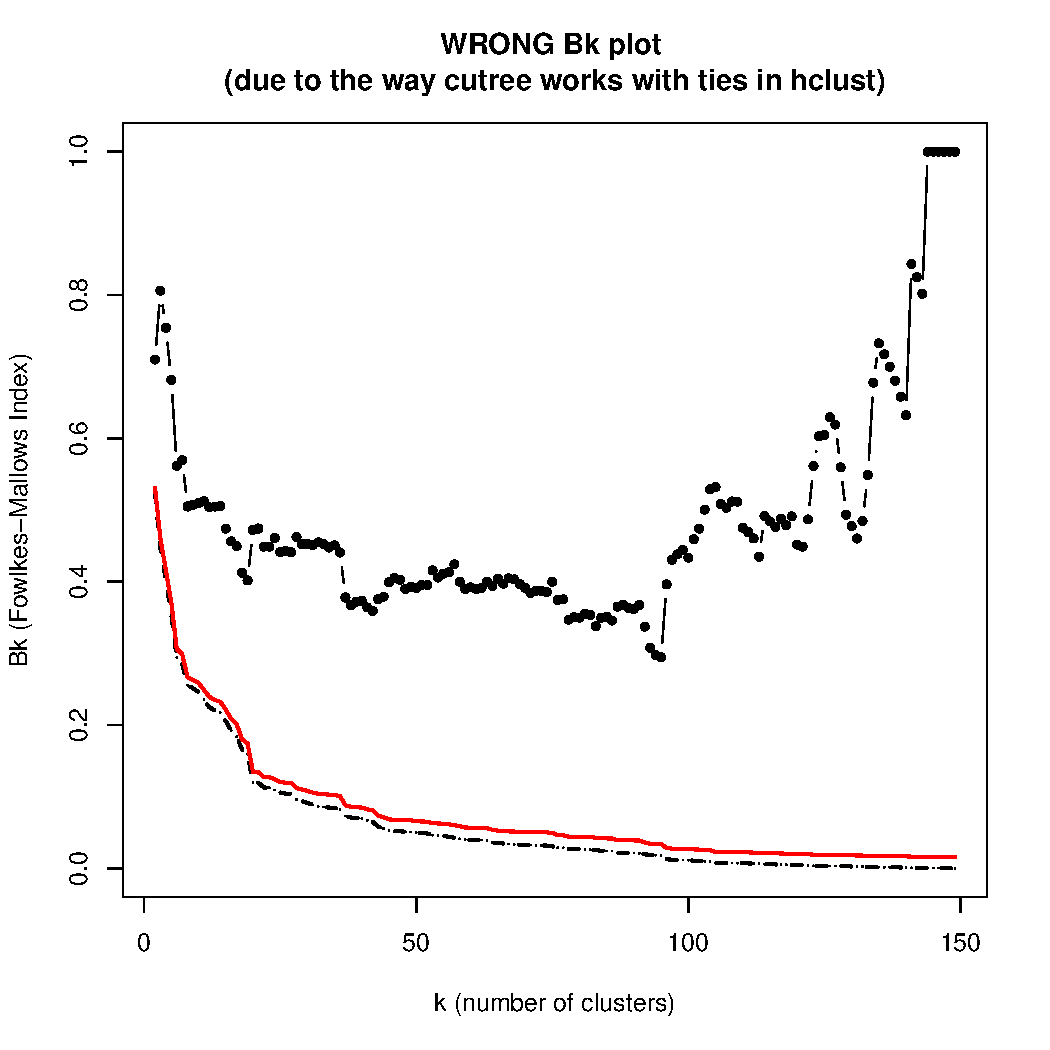
\includegraphics[width=\maxwidth]{figure/Bk_plot_for_hclust_WRONG} 

}



\end{knitrout}


\begin{knitrout}
\definecolor{shadecolor}{rgb}{0.969, 0.969, 0.969}\color{fgcolor}\begin{kframe}
\begin{alltt}
\hlkwd{Bk_plot}\hlstd{(dend1, dend2,} \hlkwc{main} \hlstd{=} \hlstr{"CORRECT Bk plot \textbackslash{}n(based on dendrograms)"}\hlstd{)}
\end{alltt}
\end{kframe}

{\centering 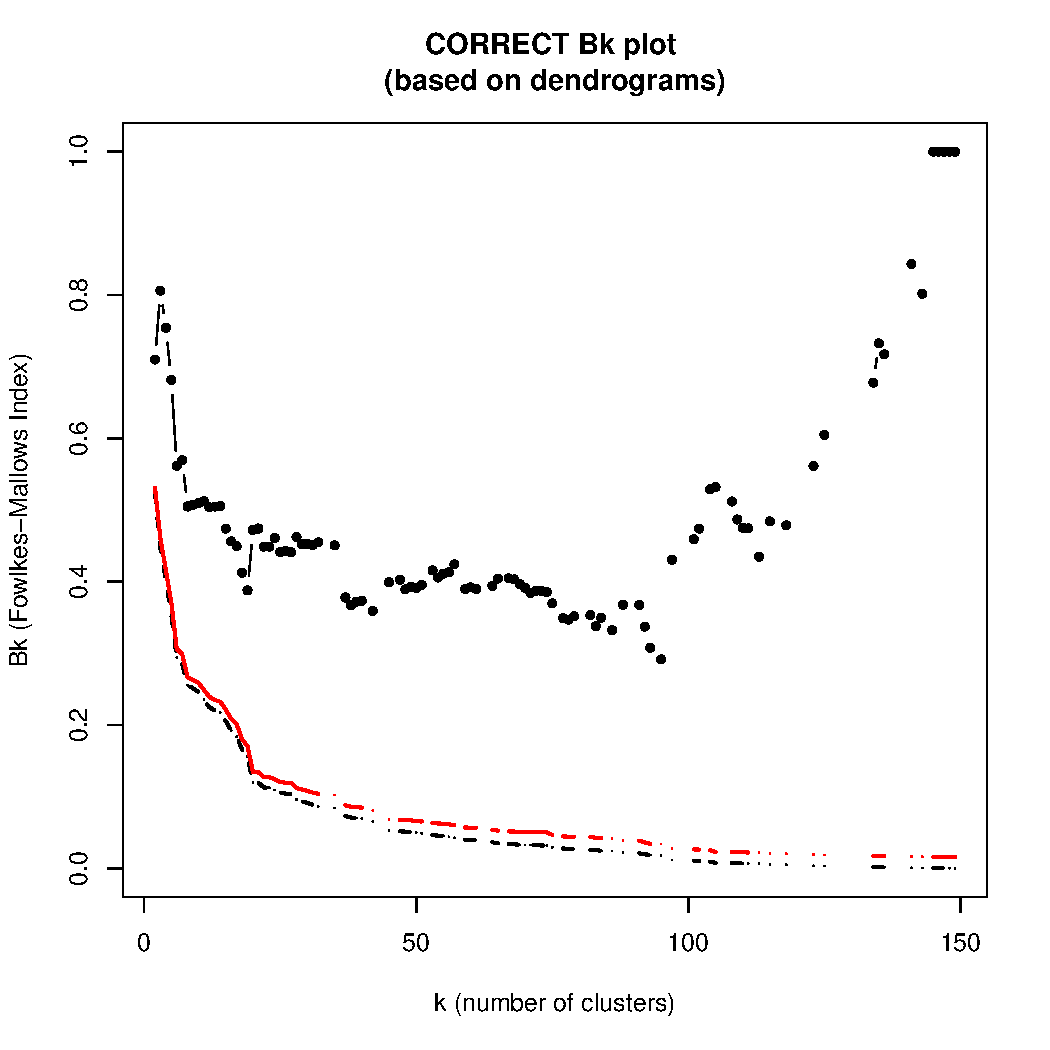
\includegraphics[width=\maxwidth]{figure/Bk_plot_for_dends_correct} 

}



\end{knitrout}




% 
% A reminder tanglegram:
% 
% <<>>=
% set.seed(2542)
% dend12_corrected_1 <- untangle_random_search(dend1, dend2,R=10)
% dend12_corrected_2 <- untangle_step_rotate_2side(dend12_corrected_1[[1]],dend12_corrected_1[[2]])
% tanglegram(dend12_corrected_2[[1]],dend12_corrected_2[[2]], margin_inner=6.5) # Better...
% 
% @
% 







\section{dendextendRcpp - gaining speed with Rcpp}

Since dendrogram objects are often revised through the use of recursion, R often falls short when it comes to speed. In various function which are intended to run only once (such as \code{labels.color}), this does not bother us, and we are content at quickly writing the function with R and let it handle many extreme cases.

However, some functions are intended to be used many times, and in such cases are well served to be handled with \proglang{C++}. Thanks the the \pkg{Rcpp} packabe (\cite{CRAN:Rcpp}, \cite{JSS:Rcpp}), we can comfortably extend several core functions of the dendextend package. These modifications are included in a seperate add-on package called \pkg{dendextendRcpp} \citep{CRAN:dendextendRcpp} by Dirk Eddelbuettel, Romain Fran\c{c}ois and Tal Galili. \pkg{dendextendRcpp} is set to load autmatically when \pkg{dendextend} loads, and its functions are set to properly override the R functions.

Here are a few benchmarks using the \pkg{microbenchmark} package \citep{CRAN:microbenchmark}.

For \code{labels.dendrogram}:

\begin{knitrout}
\definecolor{shadecolor}{rgb}{0.969, 0.969, 0.969}\color{fgcolor}\begin{kframe}
\begin{alltt}
\hlstd{dend} \hlkwb{<-} \hlkwd{as.dendrogram}\hlstd{(}\hlkwd{hclust}\hlstd{(}\hlkwd{dist}\hlstd{(iris[,} \hlopt{-}\hlnum{5}\hlstd{])))}
\hlkwd{labels}\hlstd{(dend)} \hlkwb{<-} \hlkwd{as.character}\hlstd{(}\hlkwd{labels}\hlstd{(dend)}\hlstd{)}

\hlkwd{require}\hlstd{(dendextendRcpp)}  \hlcom{# already loaded by default with dendextend}
\hlkwd{require}\hlstd{(microbenchmark)}
\hlkwd{microbenchmark}\hlstd{(stats:::}\hlkwd{labels.dendrogram}\hlstd{(dend), dendextendRcpp:::}\hlkwd{labels.dendrogram}\hlstd{(dend))}
\end{alltt}
\begin{verbatim}
## Unit: microseconds
##                                      expr     min      lq
##           stats:::labels.dendrogram(dend) 21425.4 22303.9
##  dendextendRcpp:::labels.dendrogram(dend)   543.7   560.8
##   median      uq      max neval
##  23978.2 25715.6 124609.9   100
##    700.8   719.8    931.2   100
\end{verbatim}
\begin{alltt}
# Rcpp is ~34 times faster
\end{alltt}
\end{kframe}
\end{knitrout}



For \code{get_branches_heights} (an essential function when using cutree with some k):

\begin{knitrout}
\definecolor{shadecolor}{rgb}{0.969, 0.969, 0.969}\color{fgcolor}\begin{kframe}
\begin{alltt}
\hlstd{dend} \hlkwb{<-} \hlkwd{as.dendrogram}\hlstd{(}\hlkwd{hclust}\hlstd{(}\hlkwd{dist}\hlstd{(iris[,} \hlopt{-}\hlnum{5}\hlstd{])))}
\hlkwd{labels}\hlstd{(dend)} \hlkwb{<-} \hlkwd{as.character}\hlstd{(}\hlkwd{labels}\hlstd{(dend)}\hlstd{)}

\hlkwd{require}\hlstd{(dendextendRcpp)}  \hlcom{# already loaded by default with dendextend}
\hlkwd{require}\hlstd{(microbenchmark)}
\hlkwd{microbenchmark}\hlstd{(}\hlkwd{old_get_branches_heights}\hlstd{(dend), dendextendRcpp:::}\hlkwd{get_branches_heights}\hlstd{(dend),}
    \hlkwc{times} \hlstd{=} \hlnum{100}\hlstd{)}
\end{alltt}
\begin{verbatim}
## Unit: microseconds
##                                         expr     min
##               old_get_branches_heights(dend) 51092.5
##  dendextendRcpp:::get_branches_heights(dend)   498.9
##       lq  median      uq    max neval
##  55343.3 56827.9 58136.2 149678   100
##    511.8   630.8   660.2   3561   100
\end{verbatim}
\begin{alltt}
# Rcpp is ~90 times faster!
\end{alltt}
\end{kframe}
\end{knitrout}


For \code{heights_per_k.dendrogram} (an essential function when using cutree with some k):

\begin{knitrout}
\definecolor{shadecolor}{rgb}{0.969, 0.969, 0.969}\color{fgcolor}\begin{kframe}
\begin{alltt}
\hlstd{dend} \hlkwb{<-} \hlkwd{as.dendrogram}\hlstd{(}\hlkwd{hclust}\hlstd{(}\hlkwd{dist}\hlstd{(iris[,} \hlopt{-}\hlnum{5}\hlstd{])))}
\hlkwd{labels}\hlstd{(dend)} \hlkwb{<-} \hlkwd{as.character}\hlstd{(}\hlkwd{labels}\hlstd{(dend)}\hlstd{)}

\hlkwd{require}\hlstd{(dendextendRcpp)}  \hlcom{# already loaded by default with dendextend}
\hlkwd{require}\hlstd{(microbenchmark)}
\hlkwd{microbenchmark}\hlstd{(}\hlkwd{old_heights_per_k.dendrogram}\hlstd{(dend), dendextendRcpp:::}\hlkwd{heights_per_k.dendrogram}\hlstd{(dend),}
    \hlkwc{times} \hlstd{=} \hlnum{100}\hlstd{)}
\end{alltt}
\begin{verbatim}
## Unit: milliseconds
##                                             expr     min
##               old_heights_per_k.dendrogram(dend) 3646.85
##  dendextendRcpp:::heights_per_k.dendrogram(dend)   26.41
##       lq  median      uq     max neval
##  3801.28 3924.02 3962.17 4091.29   100
##    28.36   29.55   32.14   34.91   100
\end{verbatim}
\begin{alltt}
# Rcpp is ~135 times faster!
\end{alltt}
\end{kframe}
\end{knitrout}



For \code{cut_lower_fun} (an essential function when using cutree with some h):

\begin{knitrout}
\definecolor{shadecolor}{rgb}{0.969, 0.969, 0.969}\color{fgcolor}\begin{kframe}
\begin{alltt}
\hlstd{dend_big} \hlkwb{<-} \hlkwd{as.dendrogram}\hlstd{(}\hlkwd{hclust}\hlstd{(}\hlkwd{dist}\hlstd{(iris[}\hlnum{1}\hlopt{:}\hlnum{150}\hlstd{,} \hlopt{-}\hlnum{5}\hlstd{])))}
\hlkwd{require}\hlstd{(microbenchmark)}
\hlkwd{microbenchmark}\hlstd{(}\hlkwd{old_cut_lower_fun}\hlstd{(dend_big,} \hlnum{0.01}\hlstd{), dendextendRcpp:::}\hlkwd{cut_lower_fun}\hlstd{(dend_big,}
    \hlnum{0.01}\hlstd{),} \hlkwc{times} \hlstd{=} \hlnum{100}\hlstd{)}
\end{alltt}
\begin{verbatim}
## Unit: milliseconds
##                                            expr    min
##               old_cut_lower_fun(dend_big, 0.01) 50.864
##  dendextendRcpp:::cut_lower_fun(dend_big, 0.01)  4.062
##      lq median     uq    max neval
##  60.274 66.879 76.366 239.05   100
##   4.394  4.823  5.501  39.87   100
\end{verbatim}
\begin{alltt}
# Rcpp is ~4-14 times faster. depending on the size of the
# tree, and the depth of the height
\end{alltt}
\end{kframe}
\end{knitrout}



% 
% 
% a short review of other approaches and give some historical
% background on the development of \pkg{dendextend}.
% 
% 
% Several examples are included to illustrate the functionality of \pkg{dendextend}. Many more examples are available within
% the package. % , both as explicit examples and as part of the numerous unit tests.
% %
% The \pkg{dendextend} package is available from the Comprehensive \proglang{R} Archive Network (CRAN)
% at \url{http://CRAN.R-project.org/package=dendextend}.
% 
% \makeatletter
% \if@nojss
%   This vignette will one day corresponds to a paper 
%   
% %   published in the \textsl{Journal of Statistical Software}. It is currently still identical to the published paper.  
%   
%   Over time, this vignette version may receive minor
%   updates. For citations, please use %the \cite{JSS:dendextend} or
%   % \cite{Eddelbuettel:2013:dendextend}; details are also provided in
%   \proglang{R} via \texttt{citation("dendextend")}.
% 
%   This version corresponds to \pkg{dendextend} version dendextend.version and was typeset on now.date.
% \fi
% \makeatother
% 

% \subsection{Historical context}
% \subsection{Related work}

%%% \cite - name and date in (),, \citep - (all in ())
% \cite{TempleLang:2009:RGCCTranslationUnit}, 

% \subsection[dendextend use cases]{\pkg{dendextend} use cases}
% \label{sec:classic_dendextend}

% \subsection[dendextend class hierarchy]{\pkg{dendextend} class hierarchy}
% \subsection{Derived classes}

% \subsection{Character vectors}

% \section[R and C++ data interchange]{\proglang{R} and \proglang{C++} data interchange}

% \subsection[C++ to R: wrap]{\proglang{C++} to \proglang{R}: \code{wrap}}
% \subsection[R to C++: as]{\proglang{R} to \proglang{C++}: \code{as}}

% The \citep command is used where the author name is to appear inside the parentheses alongside the date.
% \citep{Sanderson:2010:Armadillo}.


% \subsection{Implicit use of converters}

% \section{Function calls}
% \label{sec:functions}

% \section{Using code `inline'}
% \label{sec:inline}
% \code{update.packages()} 
% \footnote{This presumes a platform for which pre-built binaries are}
% \cite{CRAN:dendextend:Attributes} for more details.

% \section{Using Standard Template Library algorithms}

% \citep{Plauger+Et+Al:2000:STL}. 


% \section{Error handling}
% \subsection[C++ exceptions in R]{\proglang{C++} exceptions in \proglang{R}}
% \subsection[R errors in C++]{\proglang{R} errors in \proglang{C++}}


% \section{Performance comparison}
% \label{sec:perfcomp}



% %
% \begin{Code}
% ...
% \end{Code}
% %

% are summarized in Table~\ref{tab:benchmark} below.
% 
% \begin{table}[t]
%   \begin{center}
%     \begin{small}
%       \begin{tabular}{lrr}
%         \toprule
%         Implementation                    & Time in millisec. & Relative to \proglang{R} API \\
%         \cmidrule(r){2-3}
%         \proglang{R} API (as benchmark)             &  218       & \\
%         \pkg{dendextend} sugar                        &  145       & 0.67 \\
%         \code{NumericVector::iterator}    &  217       & 1.00 \\
%         \code{NumericVector::operator[]}  &  282       & 1.29 \\
%         %\code{dendextendVector<double>}         &  683       & 3.13 \\
%         \bottomrule
%       \end{tabular}
%     \end{small}
%     \caption{Run-time performance of the different convolution examples.}
%     \label{tab:benchmark}
%   \end{center}
% \end{table}
% 

% \section{On-going development}
% \label{sec:ongoing}

% \code{head},


\section{Summary}

The \pkg{dendextend} package presented in this paper greatly extends the available functionality of the dendrogram objects in \proglang{R}.

% compiled \proglang{C++} code with \proglang{R}.
% \pkg{dendextend} provides a \proglang{C++} class hierarchy which allows manipulation of \proglang{R} data structures in \proglang{C++}
% using member functions and operators directly related to the type
% of object being used, thereby reducing the level of expertise
% required to master the various functions and macros offered by the
% internal \proglang{R} API. The classes assume the entire
% responsibility of garbage collection of objects, relieving the
% programmer from book-keeping operations with the protection stack
% and enabling him/her to focus on the underlying problem.
% 
% Data interchange between \proglang{R} and \proglang{C++} code is performed by the \code{wrap()} and
% \code{as()} template functions. They allow the programmer to write logic in terms
% of \proglang{C++} data structures, and facilitate use of modern libraries such as the
% Standard Template Library (STL) and its containers and algorithms. The
% \code{wrap()} and \code{as()} template functions are extensible by
% design. They are also used either explicitly or implicitly throughout the API.
% By using only thin wrappers around \code{SEXP} objects and adopting \proglang{C++}
% idioms such as iterators, the footprint of the \pkg{dendextend} API
% is very lightweight, and does not incur a significant performance penalty.
% 
% The \pkg{dendextend} API offers opportunities to dramatically reduce the complexity
% of code, which should lower the initial cost of writing code and improve code readability, maintainability, and
% reuse---without incurring noticeable penalties in run-time performance.



\section*{Acknowledgments}

We are very thankful for code contributions and ideas by the R core team (especially Martin Maechler and Brian Ripley, but probably also others without our knowledge), Gavin Simpson, Gregory Jefferis
,
% Detailed comments and suggestions by editors as well as anonymous referees
% are gratefully acknowledged.  


\bibliography{dendextend-tutorial}

\vspace*{-0.35cm}




\section*{R Session Info}


\begin{knitrout}
\definecolor{shadecolor}{rgb}{0.969, 0.969, 0.969}\color{fgcolor}\begin{kframe}
\begin{alltt}
\hlkwd{Sys.Date}\hlstd{()}
\end{alltt}
\begin{verbatim}
## [1] "2013-08-31"
\end{verbatim}
\begin{alltt}
\hlkwd{sessionInfo}\hlstd{()}
\end{alltt}
\begin{verbatim}
## R version 3.0.1 (2013-05-16)
## Platform: x86_64-w64-mingw32/x64 (64-bit)
## 
## locale:
## [1] LC_COLLATE=Hebrew_Israel.1255 
## [2] LC_CTYPE=Hebrew_Israel.1255   
## [3] LC_MONETARY=Hebrew_Israel.1255
## [4] LC_NUMERIC=C                  
## [5] LC_TIME=Hebrew_Israel.1255    
## 
## attached base packages:
## [1] stats     graphics  grDevices datasets  utils    
## [6] methods   base     
## 
## other attached packages:
##  [1] profdpm_3.3          plyr_1.8            
##  [3] microbenchmark_1.3-0 colorspace_1.2-2    
##  [5] codetools_0.2-8      dendextendRcpp_0.3.0
##  [7] Rcpp_0.10.4          dendextend_0.11.2   
##  [9] ape_3.0-8            knitr_1.4           
## [11] installr_0.12.0     
## 
## loaded via a namespace (and not attached):
## [1] digest_0.6.3    evaluate_0.4.7  formatR_0.9    
## [4] grid_3.0.1      highr_0.2.2     lattice_0.20-15
## [7] nlme_3.1-109    stringr_0.6.2   tools_3.0.1
\end{verbatim}
\end{kframe}
\end{knitrout}





\end{document}

%%% Local Variables:
%%% mode: latex
%%% TeX-master: t
%%% End:


%% library(knitr)
%% Sweave2knitr('vignettes\\dendextend-tutorial.rnw')
